%yright 2007, 2008, 2009 Elsevier Ltd
%% 
%% This file is part of the 'Elsarticle Bundle'.
%% ---------------------------------------------
%% 
%% It may be distributed under the conditions of the LaTeX Project Public
%% License, either version 1.2 of this license or (at your option) any
%% later version.  The latest version of this license is in
%%    http://www.latex-project.org/lppl.txt
%% and version 1.2 or later is part of all distributions of LaTeX
%% version 1999/12/01 or later.
%% 
%% The list of all files belonging to the 'Elsarticle Bundle' is
%% given in the file `manifest.txt'.
%% 

%% Template article for Elsevier's document class `elsarticle'
%% with numbered style bibliographic references
%% SP 2008/03/01

% \documentclass[preprint,11pt]{elsarticle}
\documentclass[final,1p,11pt]{elsarticle}

%\documentclass[final,1p,times]{elsarticle}


%% Use the option review to obtain double line spacing
%%\documentclass[authoryear,preprint,review,12pt]{elsarticle}

%% Use the options 1p,twocolumn; 3p; 3p,twocolumn; 5p; or 5p,twocolumn
%% for a journal layout:
%% \documentclass[final,1p,times]{elsarticle}
%% \documentclass[final,1p,times,twocolumn]{elsarticle}
%% \documentclass[final,3p,times]{elsarticle}
%% \documentclass[final,3p,times,twocolumn]{elsarticle}
%% \documentclass[final,5p,times]{elsarticle}
%% \documentclass[final,5p,times,twocolumn]{elsarticle}

%%% For including figures, graphicx.sty has been loaded in
%% elsarticle.cls. If you prefer to use the old commands
%% please give \usepackage{epsfig}


\usepackage{epsfig}
%\usepackage{cite}
%\usepackage{mcite}
\usepackage{array,tabularx,epsfig,mathrsfs,graphicx,rotating}
\usepackage{ifthen}
\usepackage{amsfonts}
\usepackage{ragged2e}
\PassOptionsToPackage{hyphens}{url}
\usepackage[hyphens]{url}
\usepackage{hyperref}
\usepackage{listings}
\usepackage{subfigure}
\usepackage{epstopdf}
% Custom colors
\usepackage{color}
\usepackage{float}
\usepackage{verbatim}

% to cross text
\usepackage[normalem]{ulem} % either use this (simple) or
\usepackage{soul} % use this (many fancier options)


\hypersetup{
  colorlinks=true,
  linkcolor=blue,
  citecolor=blue,
  urlcolor=blue
}




\graphicspath{{figs/}}


\pdfinfo{
   /Author (Chekanov et al)
   /Title  (Studies of granularity of a hadronic calorimeter for tens-of-TeV jets  at a 100 TeV pp collider)
   /CreationDate (D:2017)
   /Subject (PDFLaTeX)
   /Keywords (PDF;LaTeX)
}


\textheight=22cm
\textwidth=14.5cm

\newcommand{\beq}{\begin{equation}}
\newcommand{\eeq}{\end{equation}}
\newcommand{\la}{\langle}
\newcommand{\promc}{{\sc ProMC}}
\newcommand{\ra}{\rangle}
\newcommand{\eps}{\epsilon}
\newcommand{\ud}{\mathrm{d}}
\newcommand{\Ec}{\mathcal{E}}
\newcommand{\Fc}{\mathcal{F}}
\newcommand{\Za}{\mathrm{Z_1}}
\newcommand{\Zb}{\mathrm{Z_2}}
\newcommand{\Zn}{\mathrm{Z_n}}
\newcommand{\F}{\mathrm{F}}

\chardef\til=126
\newcommand{\mev}{{\,\mathrm{MeV}}}
\newcommand{\gev}{{\,\mathrm{GeV}}}
\newcommand{\tev}{{\,\mathrm{TeV}}}
\newcommand{\GEANTfour} {\textsc{geant4}}
\newcommand{\pythia} {\textsc{Pythia8}}


\journal{XXX-XXX}



\begin{document}

\definecolor{mygreen}{rgb}{0,0.6,0} \definecolor{mygray}{rgb}{0.5,0.5,0.5} \definecolor{mymauve}{rgb}{0.58,0,0.82}

\lstset{ %
 backgroundcolor=\color{white},   % choose the background color; you must add \usepackage{color} or \usepackage{xcolor}
 basicstyle=\footnotesize,        % the size of the fonts that are used for the code
 breakatwhitespace=false,         % sets if automatic breaks should only happen at whitespace
 breaklines=true,                 % sets automatic line breaking
 captionpos=b,                    % sets the caption-position to bottom
 commentstyle=\color{mygreen},    % comment style
 deletekeywords={...},            % if you want to delete keywords from the given language
 escapeinside={\%*}{*)},          % if you want to add LaTeX within your code
 extendedchars=true,              % lets you use non-ASCII characters; for 8-bits encodings only, does not work with UTF-8
 keepspaces=true,                 % keeps spaces in text, useful for keeping indentation of code (possibly needs columns=flexible)
 frame=tb,
 keywordstyle=\color{blue},       % keyword style
 language=Python,                 % the language of the code
 otherkeywords={*,...},            % if you want to add more keywords to the set
 rulecolor=\color{black},         % if not set, the frame-color may be changed on line-breaks within not-black text (e.g. comments (green here))
 showspaces=false,                % show spaces everywhere adding particular underscores; it overrides 'showstringspaces'
 showstringspaces=false,          % underline spaces within strings only
 showtabs=false,                  % show tabs within strings adding particular underscores
 stepnumber=2,                    % the step between two line-numbers. If it's 1, each line will be numbered
 stringstyle=\color{mymauve},     % string literal style
 tabsize=2,                        % sets default tabsize to 2 spaces
 title=\lstname,                   % show the filename of files included with \lstinputlisting; also try caption instead of title
 numberstyle=\footnotesize,
 basicstyle=\small,
 basewidth={0.5em,0.5em}
}


\begin{frontmatter}

\title{
Studies of granularity of a hadronic calorimeter for tens-of-TeV jets  at a 100~TeV $pp$ collider 
}
%%%%%%%%%%%%%%%%%%%%%%%%%%%%%%%%%%%%%%%%%%%%%%%%%%%%%%%%%%%%%%%

\author[add1]{S.V.~Chekanov}
\ead{chekanov@anl.gov}

\author[addDuke,add2]{A.V.~Kotwal}
\ead{ashutosh.kotwal@duke.edu}

\author[add1]{J.~Proudfoot}
\ead{proudfoot@anl.gov}

\author[addDuke]{S.~Sen}
\ead{sourav.sen@duke.edu}

\author[add2]{N.V.~Tran}
\ead{ntran@fnal.gov}

\author[add3]{S.-S.~Yu}
\ead{syu@cern.ch}

\author[add3]{Chih-Hsiang Yeh}
\ead{jwzuzelski18@gmail.com}

\address[add1]{
HEP Division, Argonne National Laboratory,
9700 S.~Cass Avenue,
Argonne, IL 60439, USA. 
}

\address[addDuke]{
Department of Physics, Duke University, USA
}

\address[add2]{
Fermi National Accelerator Laboratory
}

\address[addMSU]{
Department of Physics, Michigan State University, 220
Trowbridge Road, East Lansing, MI 48824 
}


\address[add3]{
Department of Physics, National Central University, Chung-Li, Taoyuan City 32001, Taiwan
}


\begin{abstract}
Texts

\end{abstract}

\begin{keyword}
multi-TeV physics, $pp$ collider, future hadron colliders, FCC, SppC
\end{keyword}



\end{frontmatter}


% put line numbers
% \linenumbers

%%%%%%%%%%%%%%%%%%%%%%%%%%%%%%%%%%%%%%%%%%%%%%%%%%%%%%%%%%%%%%%%%%
\section{Introduction}
%%%%%%%%%%%%%%%%%%%%%%%%%%%%%%%%%%%%%%%%%%%%%%%%%%%%%%%%%%%%%%%%%%

Particle collisions at energies  beyond those attained at the LHC will lead to many challenges for detector technologies.
Future experiments, such as high-energy LHC (HE-LHC),
future circular $pp$ colliders of the European initiative, FCC-hh~\cite{Benedikt:2206376} and the Chinese initiative, SppC~\cite{Tang:2015qga} will be required to measure high-momentum bosons ($W$, $Z$, $H$) and top quarks with strongly 
collimated decay products that form jets.  Studies of jet substructure can help identify such particles.

The reconstruction of jet substructure  variables for collimated jets with transverse momentum above 10 TeV 
require an appropriate detector design. The most important for reconstruction of such jets are tracking and calorimeter.
Recently, a number of studies \cite{Calkins:2013ega,Chekanov:2015ihl,Coleman:2017fiq} 
have been discussed using various fast simulation tools, such as 
Delphes  \cite{deFavereau:2013fsa}, in which momenta of particles
are smeared to mimic detector response. 

A major step towards the usage of full Geant4 simulation to verify the granularity requirements 
for calorimeters was made in \cite{Chekanov:2016ppq}.
The studies included in this paper have illustrated a significant impact 
of granularity of electromagnetic (ECAL) and hadronic (HCAL) calorimeters on the
shape of hadronic showers  calculated using calorimeter hits 
for two particles separated  by some angle. It was concluded that high granularity is essential 
in resolving two close-by particles for energies above 100 GeV. 

This paper makes another step in understanding understanding of this problem in terms 
of high-level physics quantities typically used in physics analyses.
Similar to the studies presented in \cite{Chekanov:2016ppq}, this paper is based on full
Geant4 simulation with realistic jet reconstruction.

\section{Simulation of detector response and event reconstruction}
 
The description of the detector and software used for this paper is discussed in \cite{Chekanov:2016ppq}. 
We use the SiFCC detector geometry with a software package that
represents a versatile environment for simulations
of detector performance, testing new technology options, event reconstruction techniques for future
100~TeV colliders.

The \GEANTfour\ (version 10.3)~\cite{Allison2016186} simulation of calorimeter response was complemented 
with the full reconstruction of calorimeter clusters formed by the Pandora algorithm \cite{Charles:2009ta,Marshall:2013bda}.
Calorimeter clusters were built from calorimeter hits in the  ECAL and HCAL after applying the corresponding sampling fractions.
No other corrections are applied.
Hadronic jets were 
reconstructed with the {\sc FastJet} package~\cite{fastjet} using the anti-$k_T$ algorithm \cite{Cacciari:2008gp}
with  a distance parameter of 0.5. 

In the following discussion, we use the simulations of a heavy $Z'$ boson, 
a hypothetical gauge boson  that arises from extensions of the electroweak symmetry of the Standard Model.
The $Z'$ bosons were simulated with the masses, $M=5$, $10$, $20$ and $40$~TeV. The lowest value 
represents a typical mass that is within the reach of the LHC experiments. The  value $40$~TeV 
represents the physics reach of 100~TeV colliders. The $Z'$ particles are forced to decay to 
to two light-flavor jets ($q\bar{q}$), $W^+W^-$ or $t\bar{t}$, where
$W$ and $t$ decay hadronically. In all such scenarios, two highly boosted
jets are produced,  which are typically back-to-back in the laboratory frame.
Typical transverse momenta of such jets are $\simeq M/2$.
The main difference between considered decay types lays in different jet substructure. In the case of the $q\bar{q}$ decays,
jets do not have any internal structure. In the case of  $W^+W^-$, each jet  originates from $W$, thus it has two
subjects because of the decay $W\rightarrow q\bar{q}$. In the case of hadronic top decays, jets have three subjects due
to the decay $t \rightarrow  W^+\>b \rightarrow q\bar{q} b$    
The signal events were generated using the \pythia generator with the default settings,
ignoring interference with SM processes.
The event samples used in this paper are  available from the
HepSim  database~\cite{Chekanov:2014fga}.



%%%%%%%%%%%%%% sections 
\section{Studies of jet properties}
\label{sec:jets}

First let us consider several variables that represent jet substructure using different types
of calorimeter granularity. The question we want to answer is how close the reconstructed
jet substructure variables to the input "truth" value that are reconstructed using 
input particles directly from the \pythia generator.


The effective radius is the average of the energy weighted radial distance in $\eta-\phi$ space of jet constituents.
Recently, it has been studied for multi-TeV jets in Ref.\cite{Auerbach:2014xua}.
 

\begin{figure}
\begin{center}
   \subfigure[5 TeV] {
   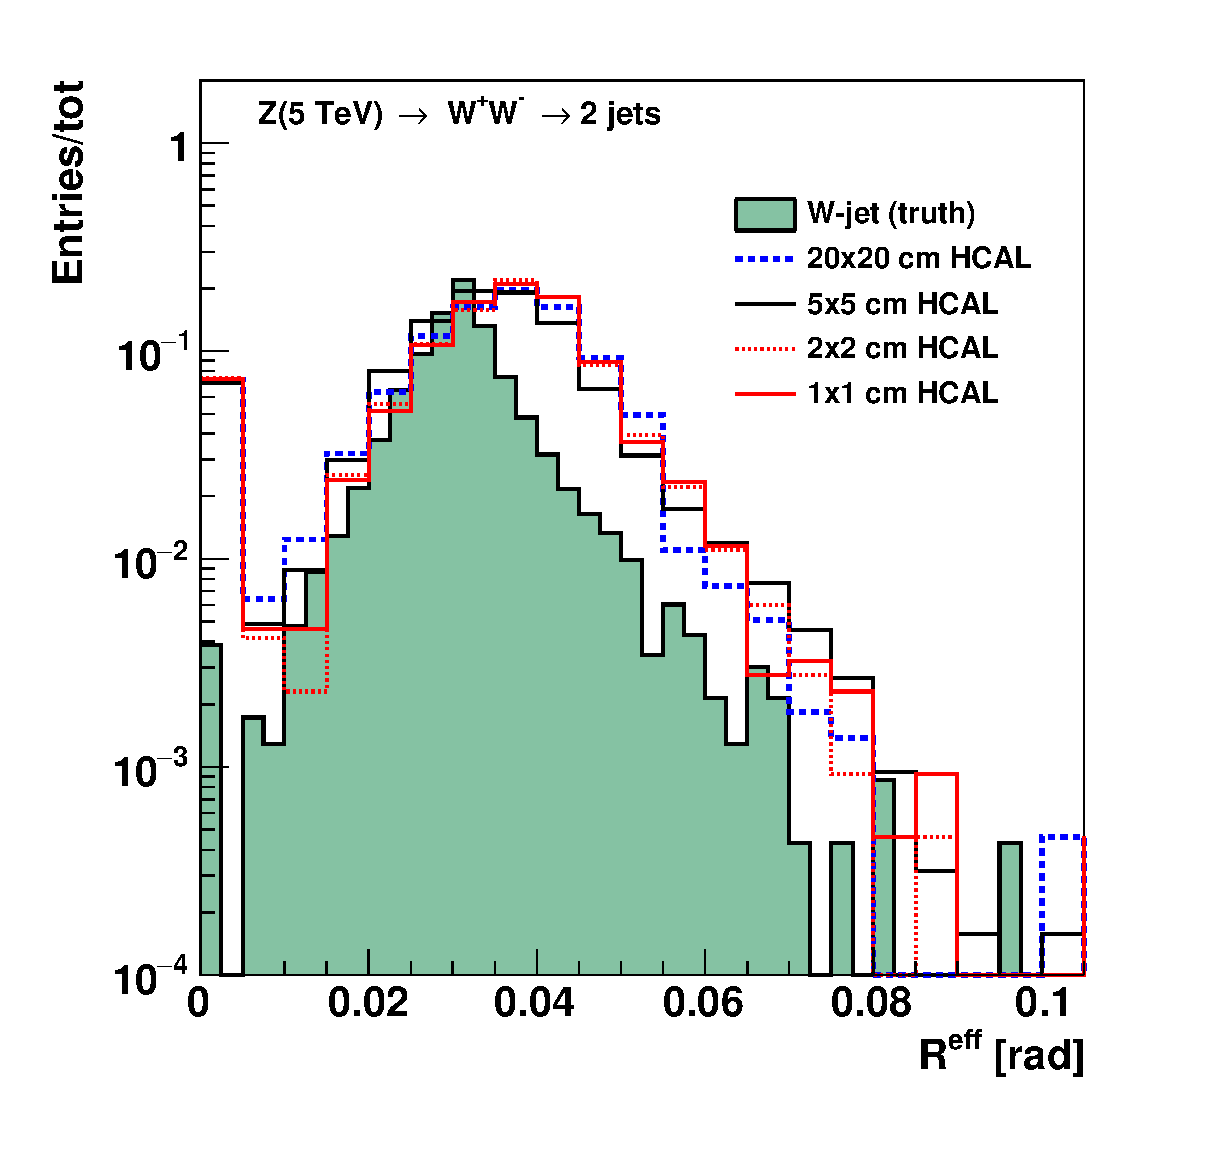
\includegraphics[width=0.43\textwidth]{figs/h5tev_clus_effR_ww1}\hfill
   }
   \subfigure[10 TeV] {
   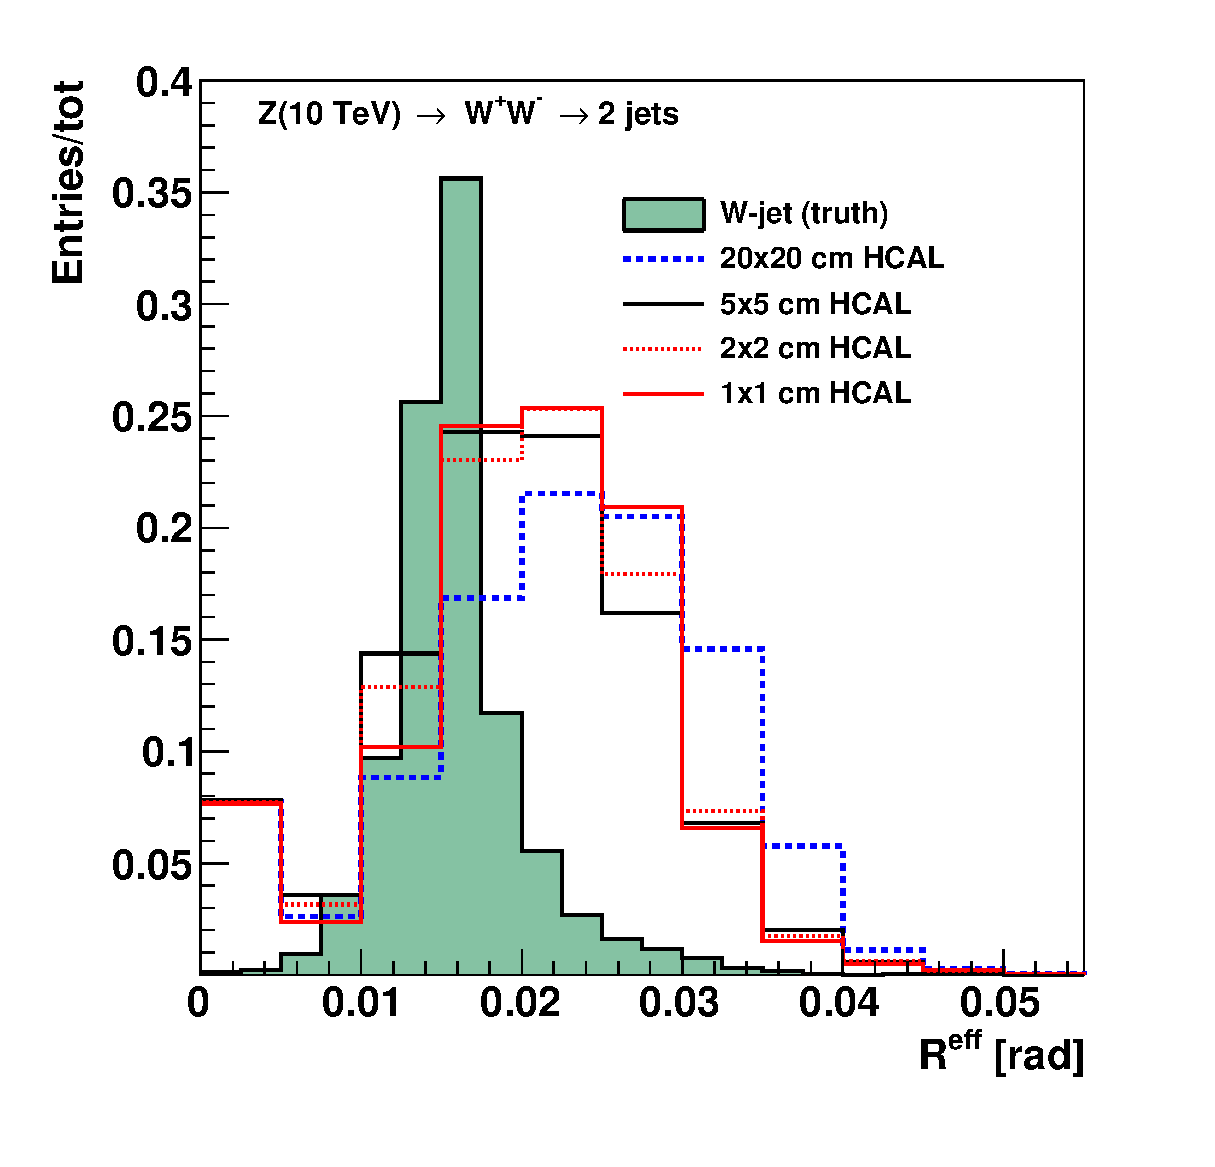
\includegraphics[width=0.43\textwidth]{figs/h10tev_clus_effR_ww1}
   }
   \subfigure[20 TeV] {
   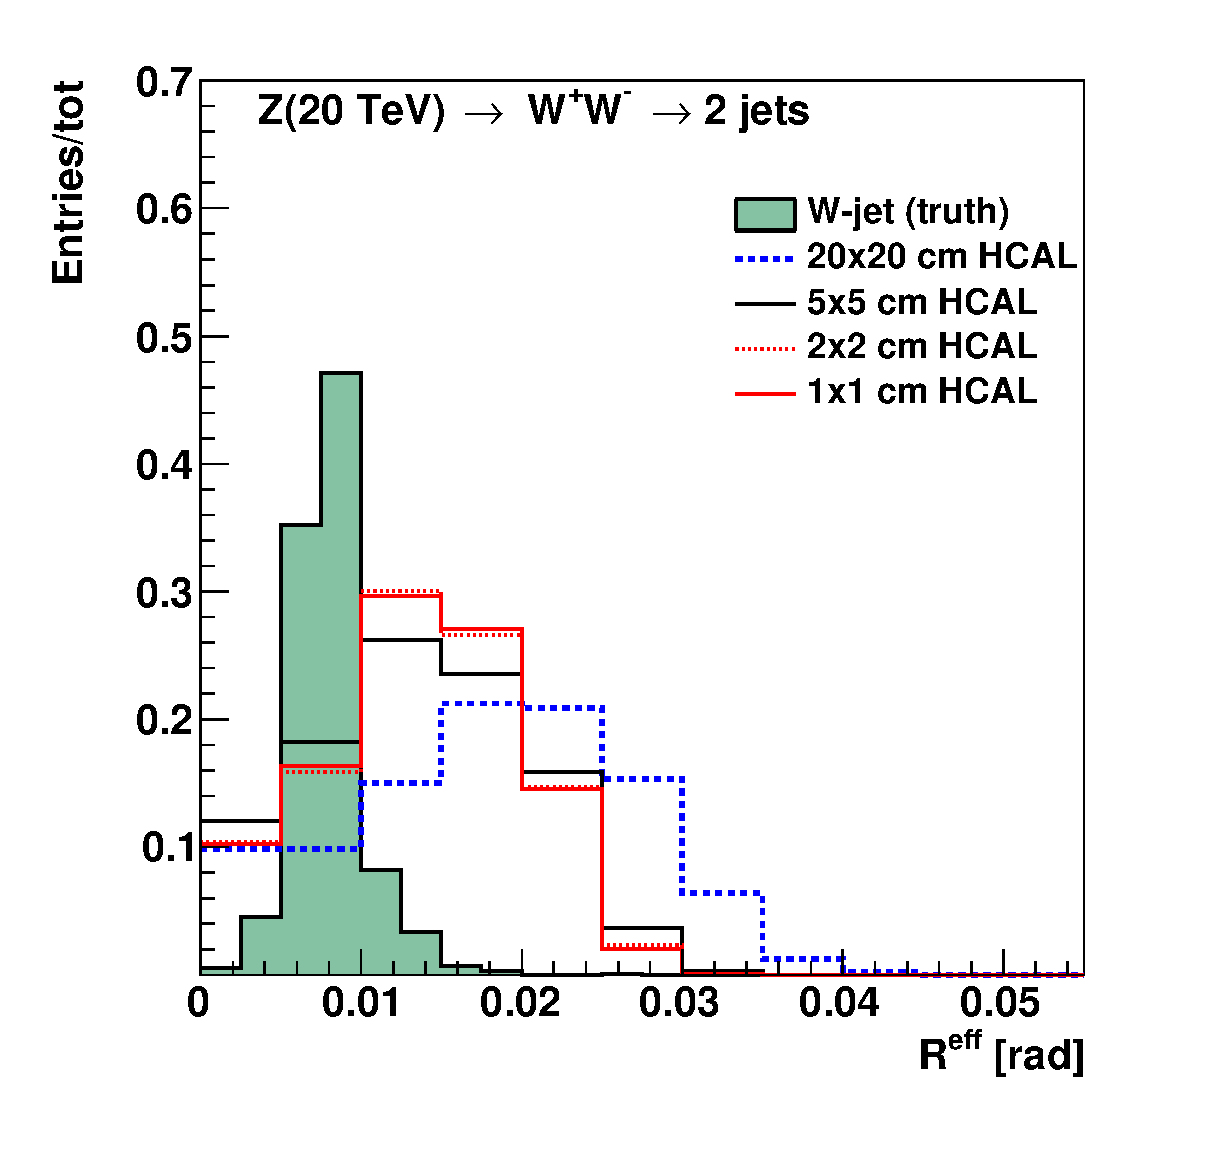
\includegraphics[width=0.43\textwidth]{figs/h20tev_clus_effR_ww1}
   }
   \subfigure[40 TeV] {
   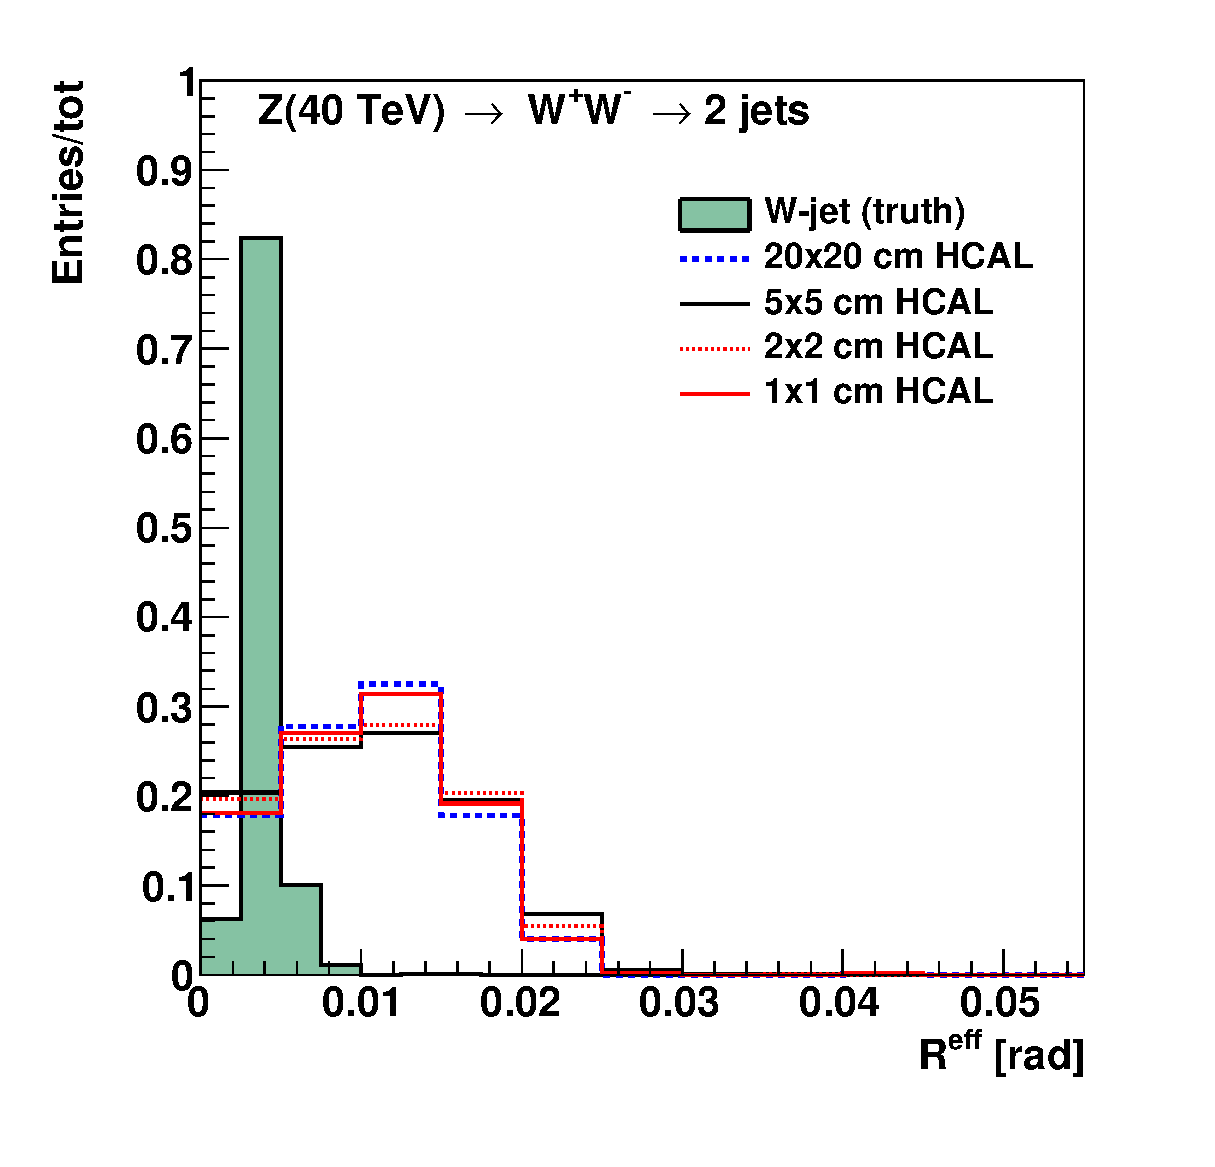
\includegraphics[width=0.43\textwidth]{figs/h40tev_clus_effR_ww1}
   }
\end{center}
\caption{Jet effective radius for different jet transverse moment and HCAL granularity.}
\label{fig:eff_rad}
\end{figure}


Let us study the effect of granularity on jet splitting scales.
A jet $k_T$ splitting scale \cite{Butterworth:2002tt} is defined as a distance measure
used to form jets by the $k_T$ recombination
algorithm \cite{Catani1993187,Ellis:1993tq}.
This has been studied by ATLAS~\cite{ATLAS:2012am}, and more recently in the context of 100 TeV physics \cite{Auerbach:2014xua}.
The distribution of the splitting scale $\sqrt{d_{12}}=\min(p_T^1,p_T^2) \times \delta R_{12}$ \cite{ATLAS:2012am} at the final stage of the $k_T$ clustering, where two subjets are merged into the final one,
is shown in Fig.~\ref{fig:d12}.

\begin{figure}
\begin{center}
   \subfigure[5 TeV] {
   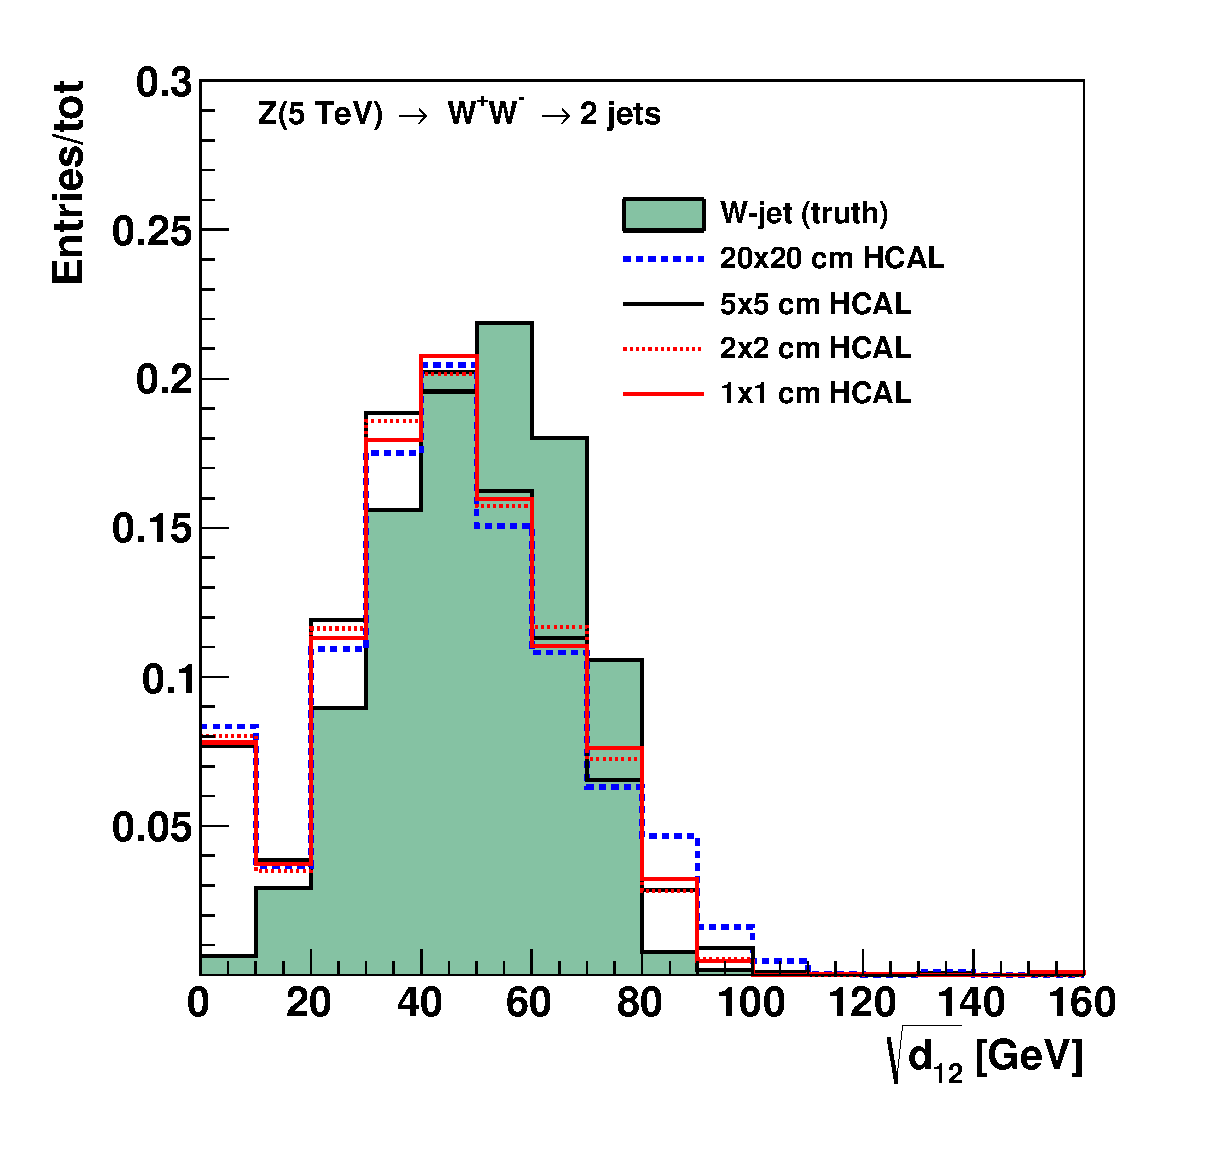
\includegraphics[width=0.43\textwidth]{figs/h5tev_clus_d12_ww1}\hfill
   }
   \subfigure[10 TeV] {
   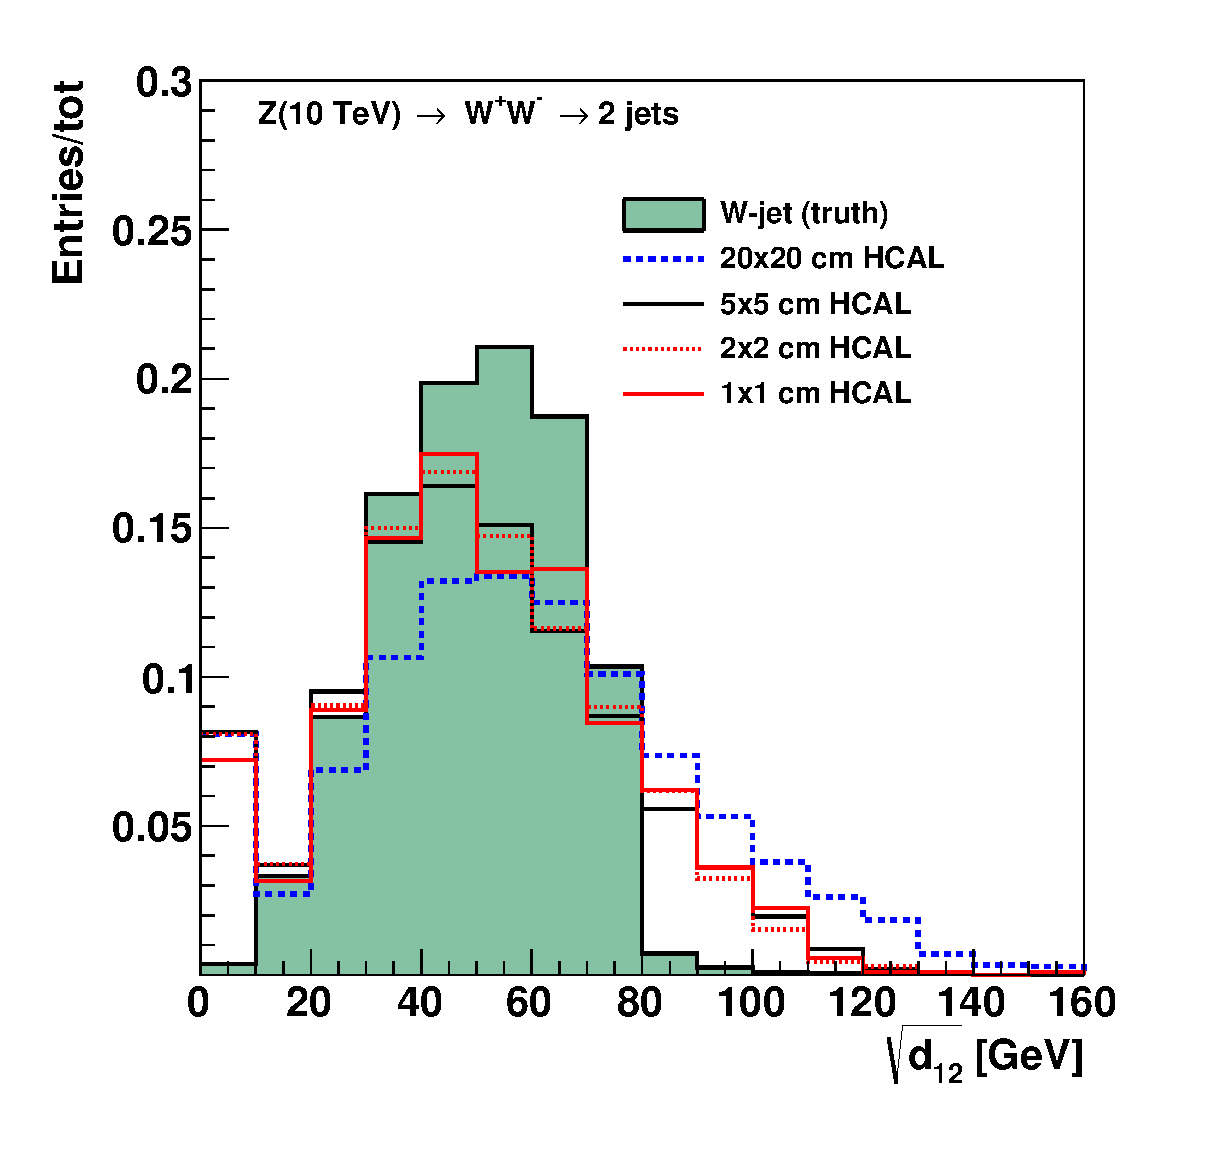
\includegraphics[width=0.43\textwidth]{figs/h10tev_clus_d12_ww1}
   }
   \subfigure[20 TeV] {
   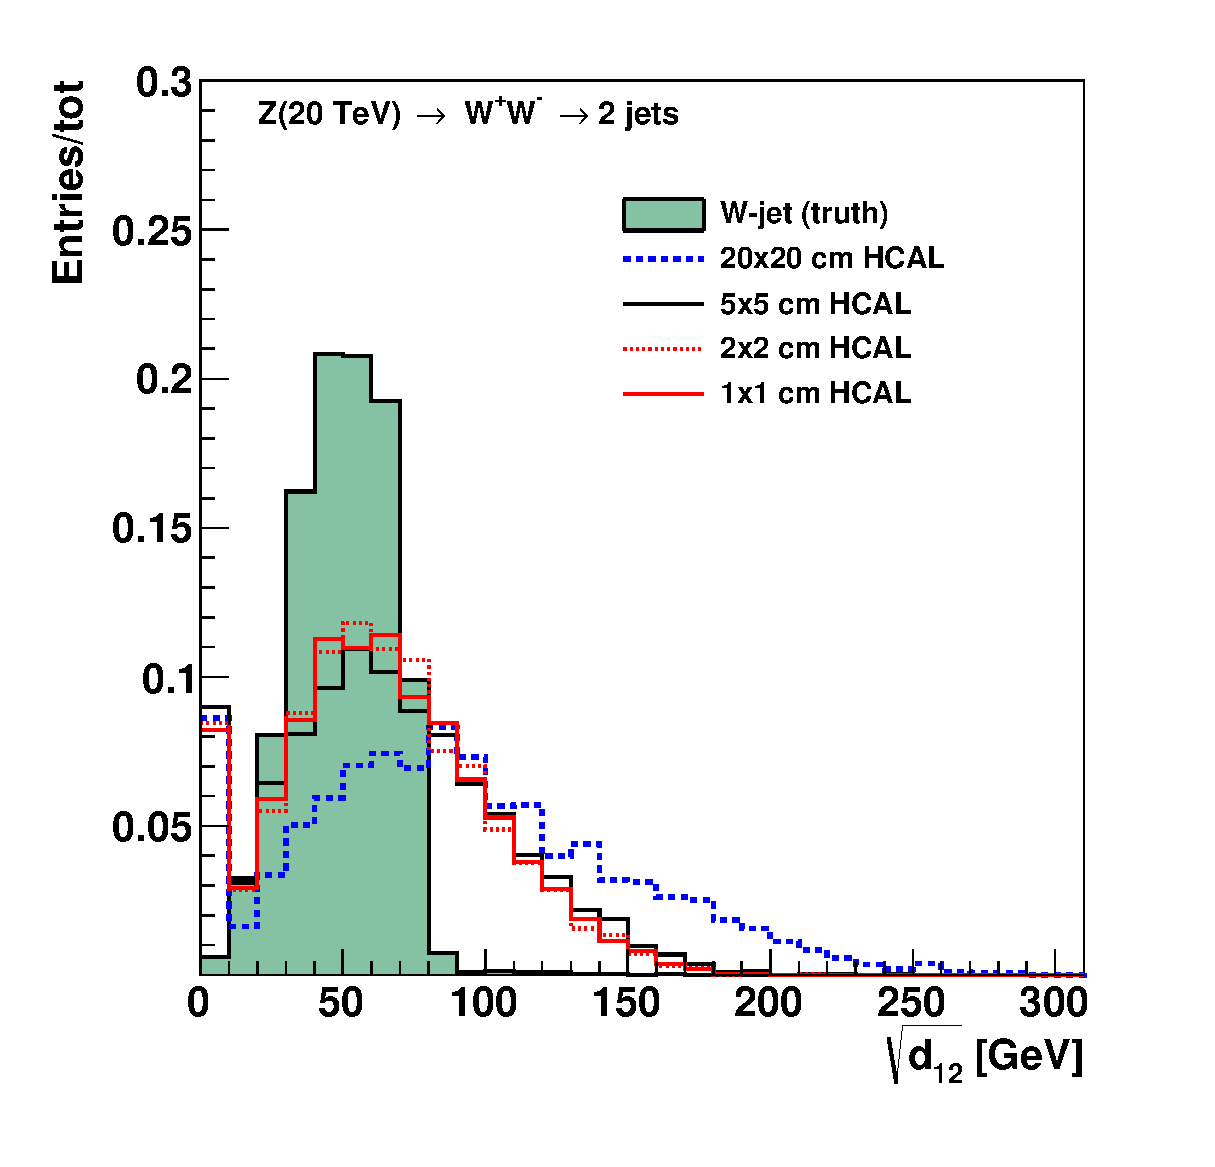
\includegraphics[width=0.43\textwidth]{figs/h20tev_clus_d12_ww1}
   }
   \subfigure[40 TeV] {
   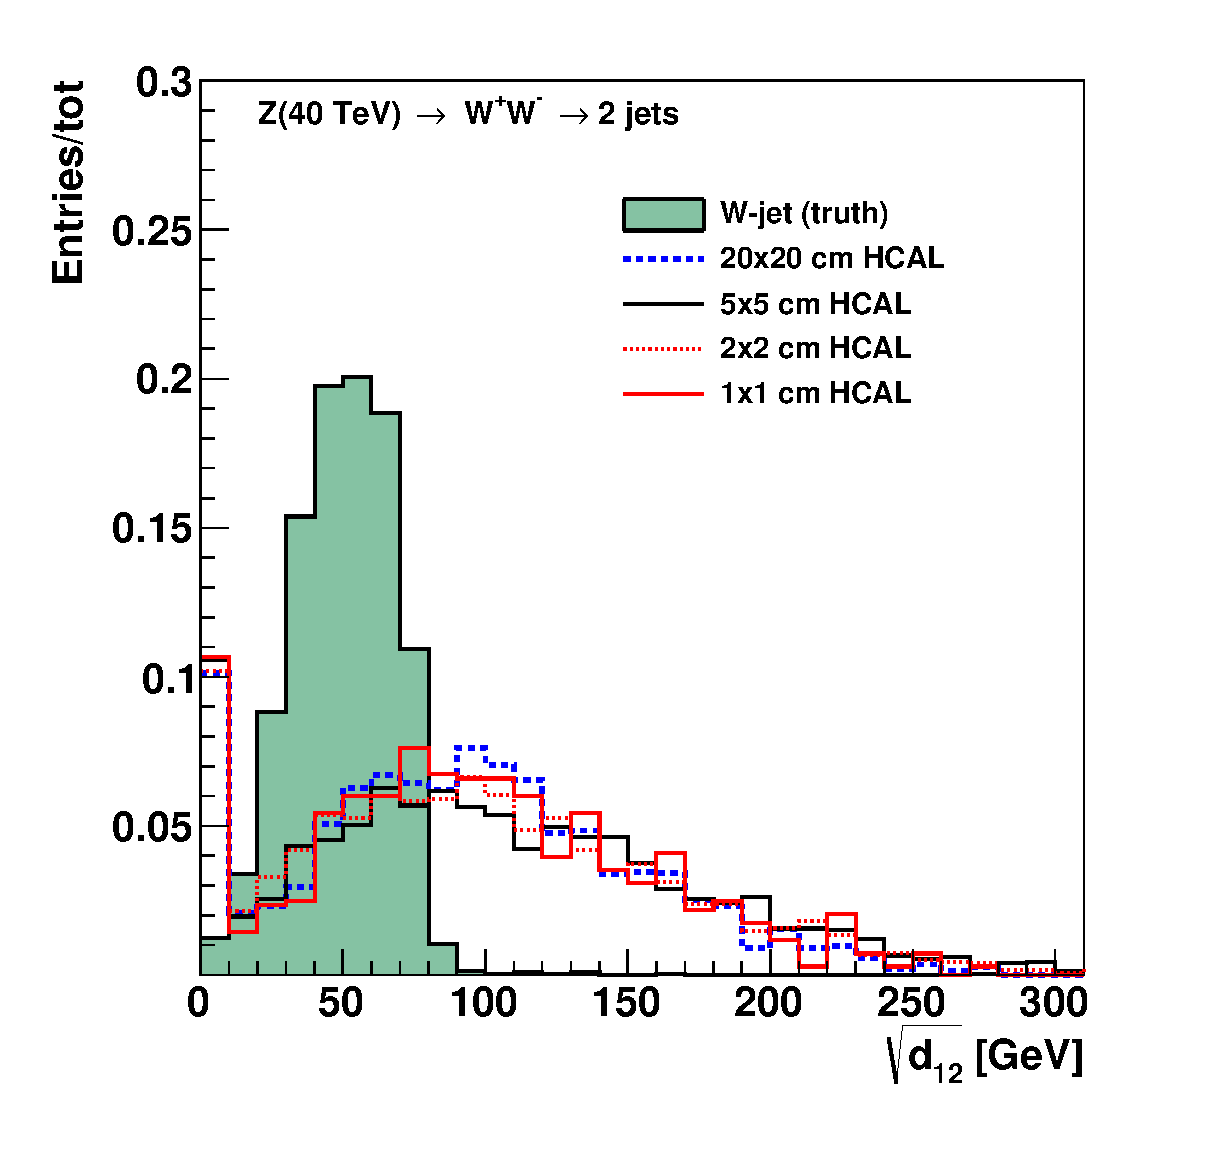
\includegraphics[width=0.43\textwidth]{figs/h40tev_clus_d12_ww1}
   }
\end{center}
\caption{Jet splitting scale for different jet transverse moment and HCAL granularity.}
\label{fig:d12}
\end{figure}


\subsection{Jet subjettiness}

We recall that $N$-subjettiness~\cite{Ellis:2009su,Thaler:2010tr}, $\tau_{N}$, of jets has been proposed
as a class of variables with which to study the decay products of a heavy particle inside jets.  $\tau_{N}$ is a measure of the degree to which a jet can be considered as being composed of
 $N$  $k_{T}$-subjets \cite{Thaler:2010tr}. 
The variable $\tau_{32}$, defined as the ratio of the $N$-subjettiness variables $\tau_3/\tau_2$, is particularly sensitive to hadronically-decaying
 top-quark initiated jets.
The variable, $\tau_{21} \equiv \tau_2/\tau_1$ can be used to reject background from $W/Z$ decays.
These variables do not strongly correlate with jet mass and can provide an independent check for the
presence of top quarks.
The jet substructure variables were obtained by re-running the $k_T$ algorithm over the jet constituents of anti-$k_T$ jets.

%%%%%%%%%%%%%%% commented out 
\begin{comment}


As an example of the effect of the calorimeter granularity, 
\begin{figure}
\begin{center}
   \subfigure[5 TeV] {
   \includegraphics[width=0.43\textwidth]{figs/r09_tau21b1_20tev_04_U.pdf}\hfill
   }
   \subfigure[10 TeV] {
   \includegraphics[width=0.43\textwidth]{figs/r010_tau21b1_20tev_04_U.pdf}
   }
   \subfigure[20 TeV] {
   \includegraphics[width=0.43\textwidth]{figs/r012_tau21b1_20tev_04_U.pdf}
   }
\end{center}
\caption{Jet subjetinness $\tau_{21}$ for jets originating from splitting scale for different jet transverse moment and HCAL granularity.}
\label{fig:tau21}
\end{figure}


\begin{figure}
\begin{center}
   \subfigure[5 TeV] {
   \includegraphics[width=0.43\textwidth]{figs/r09_tau32b1_20tev_04_U.pdf}\hfill
   }
   \subfigure[10 TeV] {
   \includegraphics[width=0.43\textwidth]{figs/r010_tau32b1_20tev_04_U.pdf}
   }
   \subfigure[20 TeV] {
   \includegraphics[width=0.43\textwidth]{figs/r012_tau32b1_20tev_04_U.pdf}
   }
\end{center}
\caption{Jet subjetinness $\tau_{32}$ for jets originating from splitting scale for different jet transverse moment and HCAL granularity.}
\label{fig:tau21}
\end{figure}

%%%%%%%%%%%%%%% commented out 
\end{comment}



%yright 2007, 2008, 2009 Elsevier Ltd
%% 
%% This file is part of the 'Elsarticle Bundle'.
%% ---------------------------------------------
%% 
%% It may be distributed under the conditions of the LaTeX Project Public
%% License, either version 1.2 of this license or (at your option) any
%% later version.  The latest version of this license is in
%%    http://www.latex-project.org/lppl.txt
%% and version 1.2 or later is part of all distributions of LaTeX
%% version 1999/12/01 or later.
%% 
%% The list of all files belonging to the 'Elsarticle Bundle' is
%% given in the file `manifest.txt'.
%% 

%% Template article for Elsevier's document class `elsarticle'
%% with numbered style bibliographic references
%% SP 2008/03/01

% \documentclass[preprint,11pt]{elsarticle}
\section{Soft drop method in future collider performance}
In this section, we use the specific method about the soft-drop to study the performance of the detector in the different cell sizes.  In the Figure , , , , are the distribution of the signal and background. 
\subsection{Analysis method}
In this analysis, We fix the central at the median in signal distribution, and we use the different width to open the window to draw ROC curves.
\subsection{The conclusion of the results}

 
%50bins
\begin{figure}
\begin{center}
   \subfigure[5TeV at 20$\times$20(cm$\times$cm) in cluster] {
   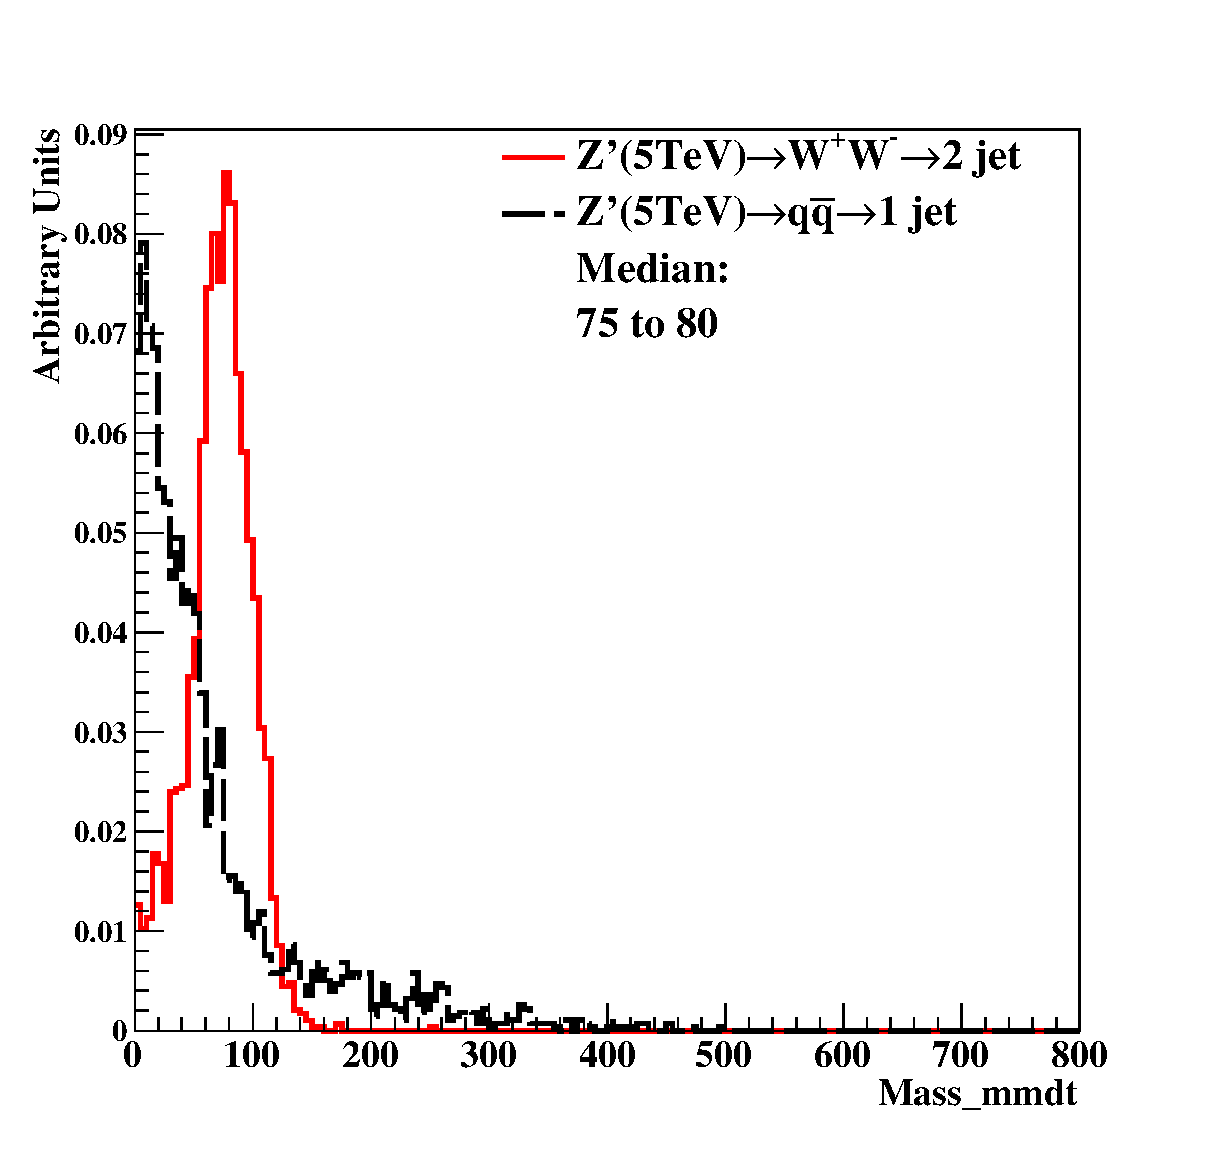
\includegraphics[width=0.22\textwidth]{figs/Dis_cluster_010_mass_mmdt_5tev_04.eps}
   }
      \subfigure[10TeV at 20$\times$20(cm$\times$cm) in cluster] {
   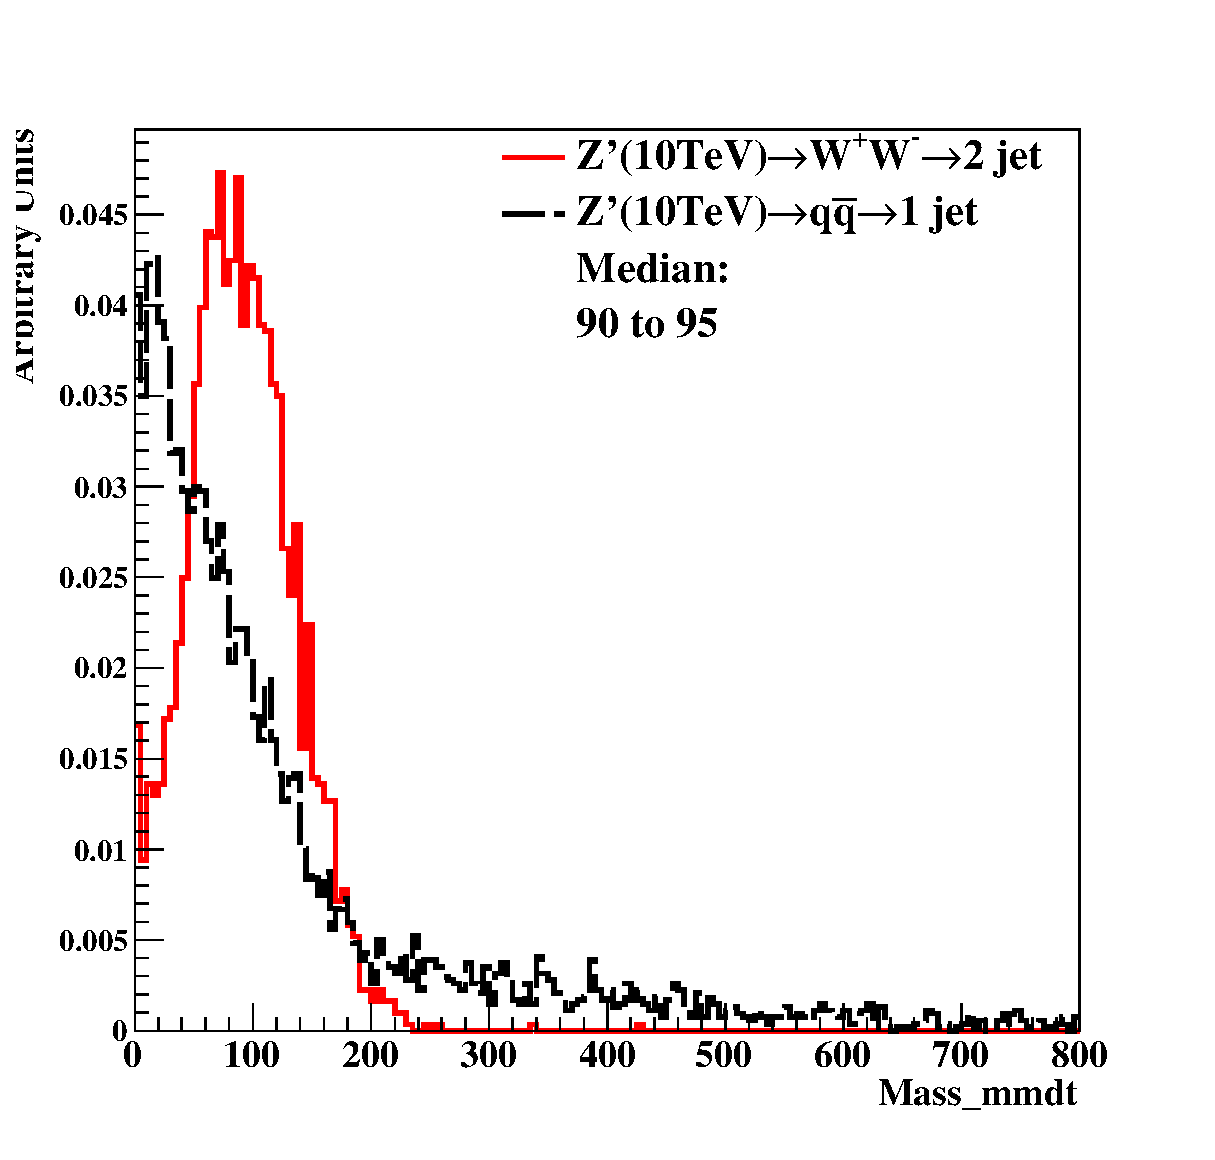
\includegraphics[width=0.22\textwidth]{figs/Dis_cluster_010_mass_mmdt_10tev_04.eps}
   }
   \subfigure[20TeV at 20$\times$20(cm$\times$cm) in cluster] {
   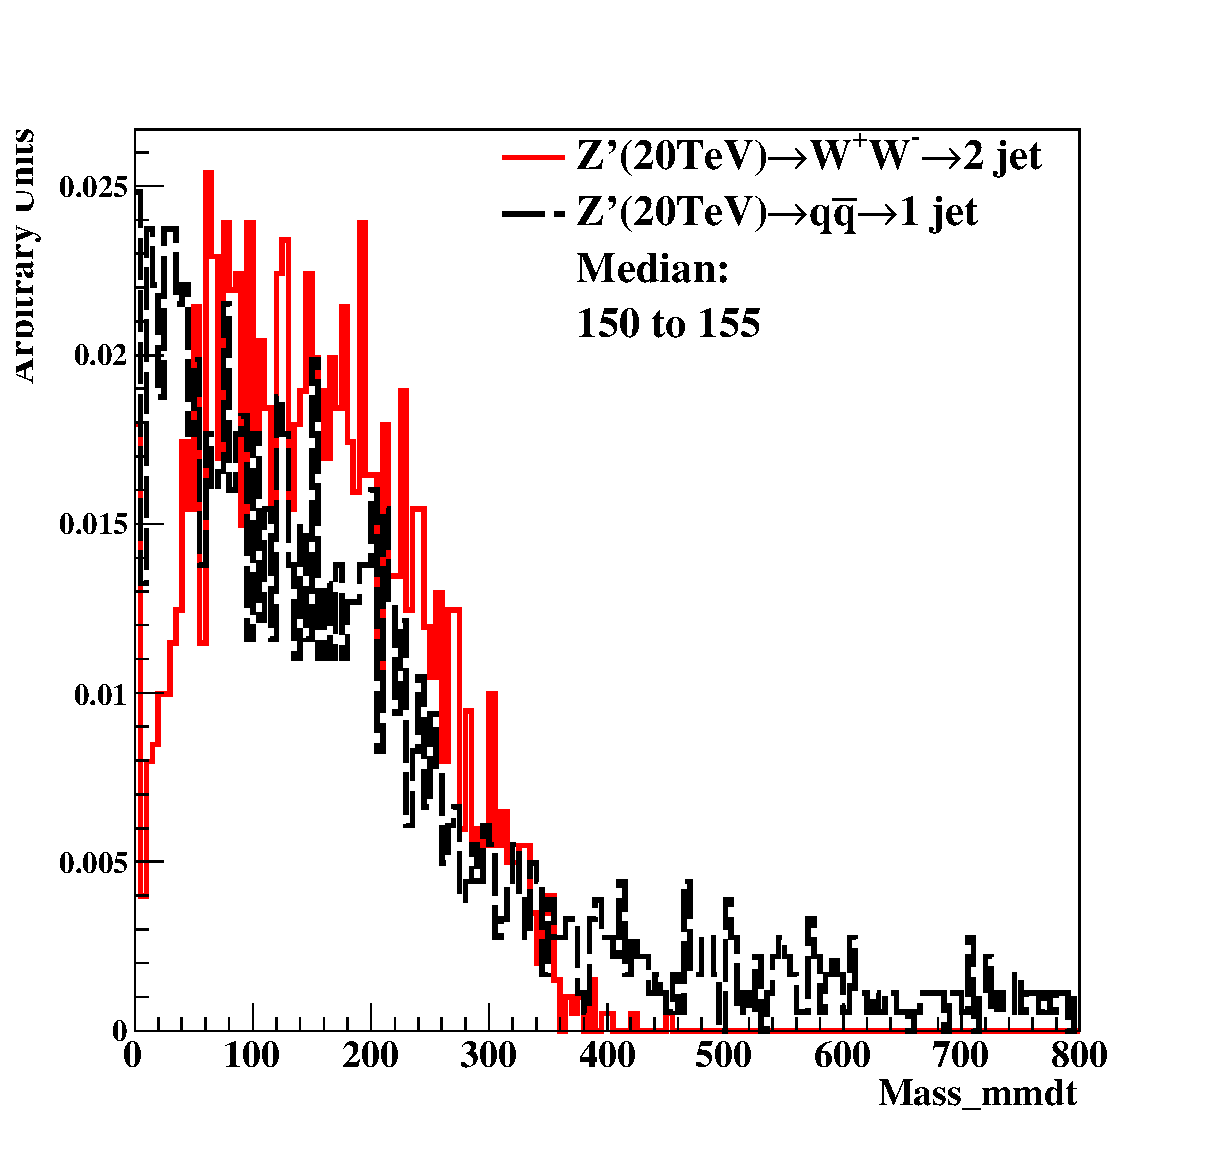
\includegraphics[width=0.22\textwidth]{figs/Dis_cluster_010_mass_mmdt_20tev_04.eps}
   }
    \subfigure[40TeV at 20$\times$20(cm$\times$cm) in cluster] {
   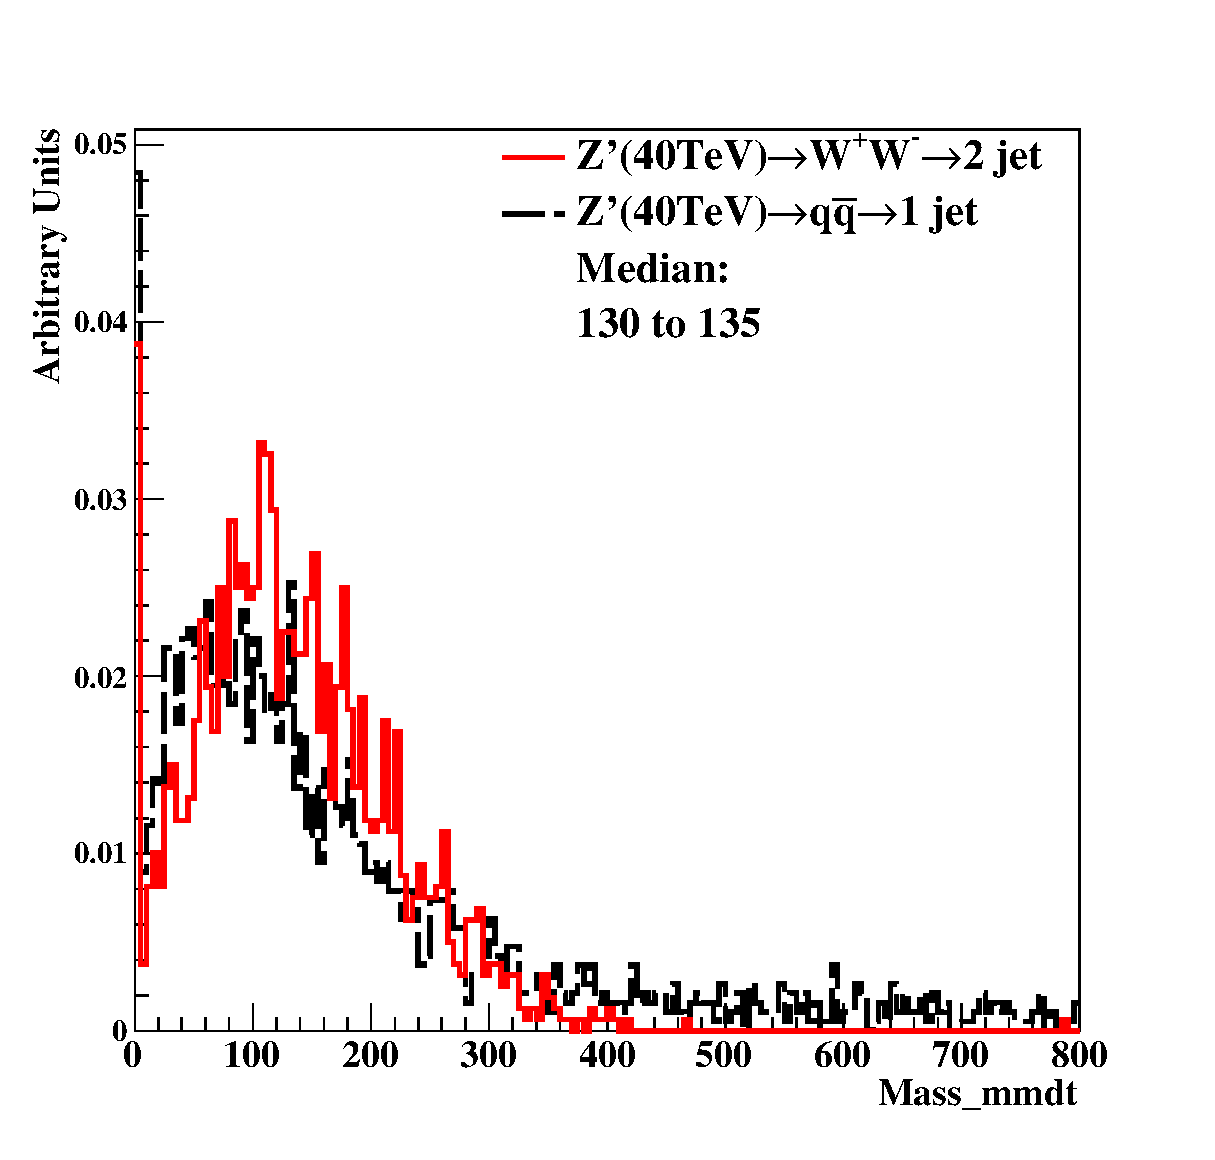
\includegraphics[width=0.22\textwidth]{figs/Dis_cluster_010_mass_mmdt_40tev_04.eps}
   }
   \subfigure[5TeV at 5$\times$5(cm$\times$cm) in cluster] {
   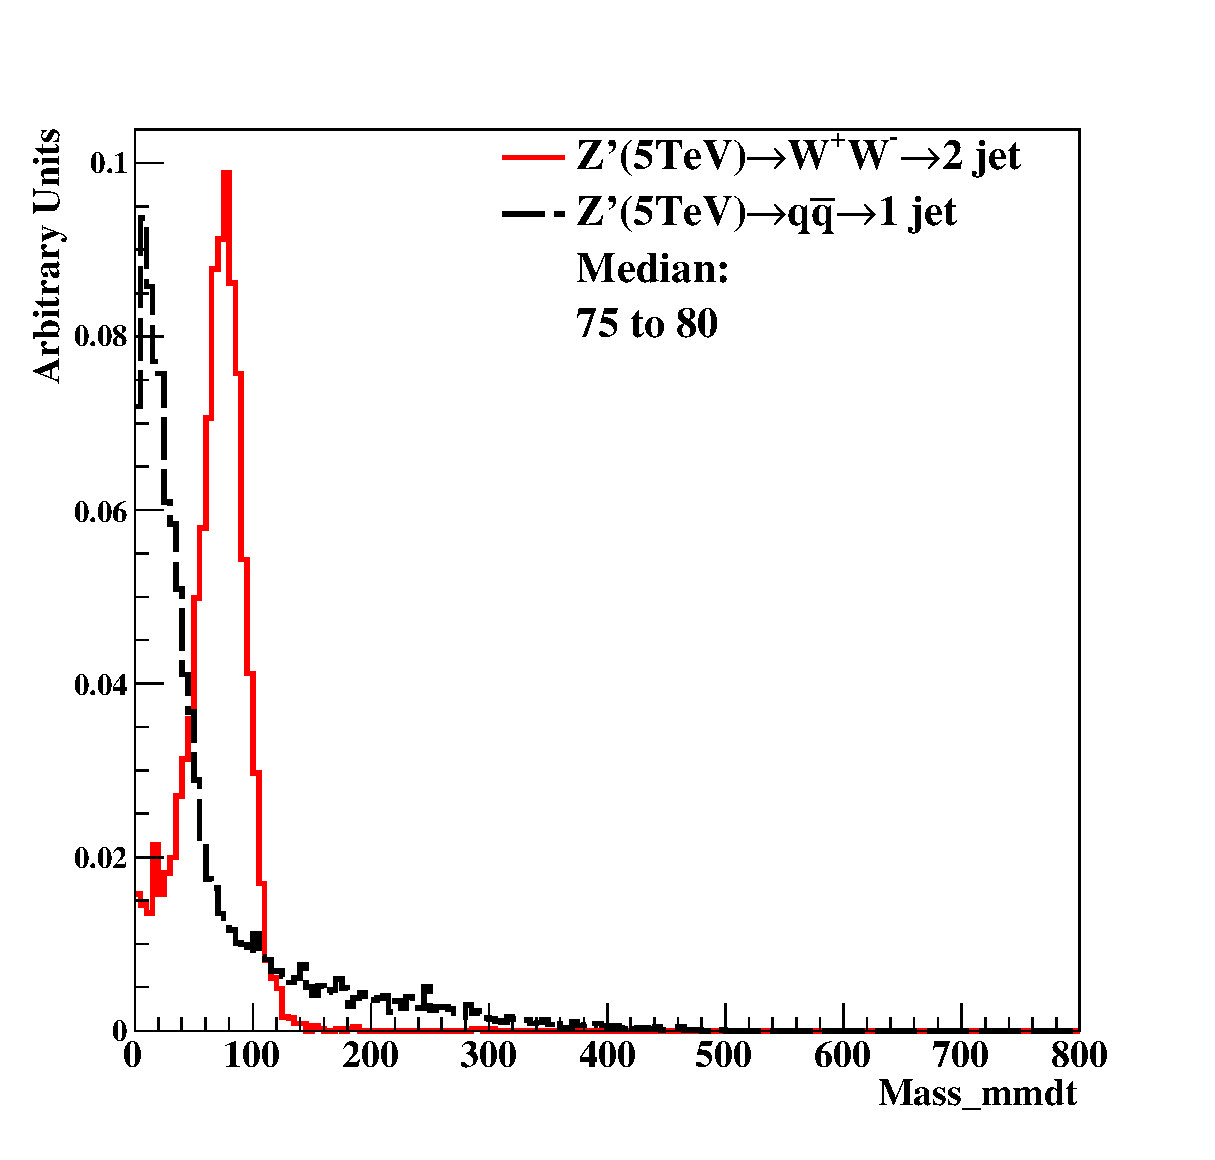
\includegraphics[width=0.22\textwidth]{figs/Dis_cluster_009_mass_mmdt_5tev_04.eps}
   }
   \subfigure[10TeV at 5$\times$5(cm$\times$cm) in cluster] {
   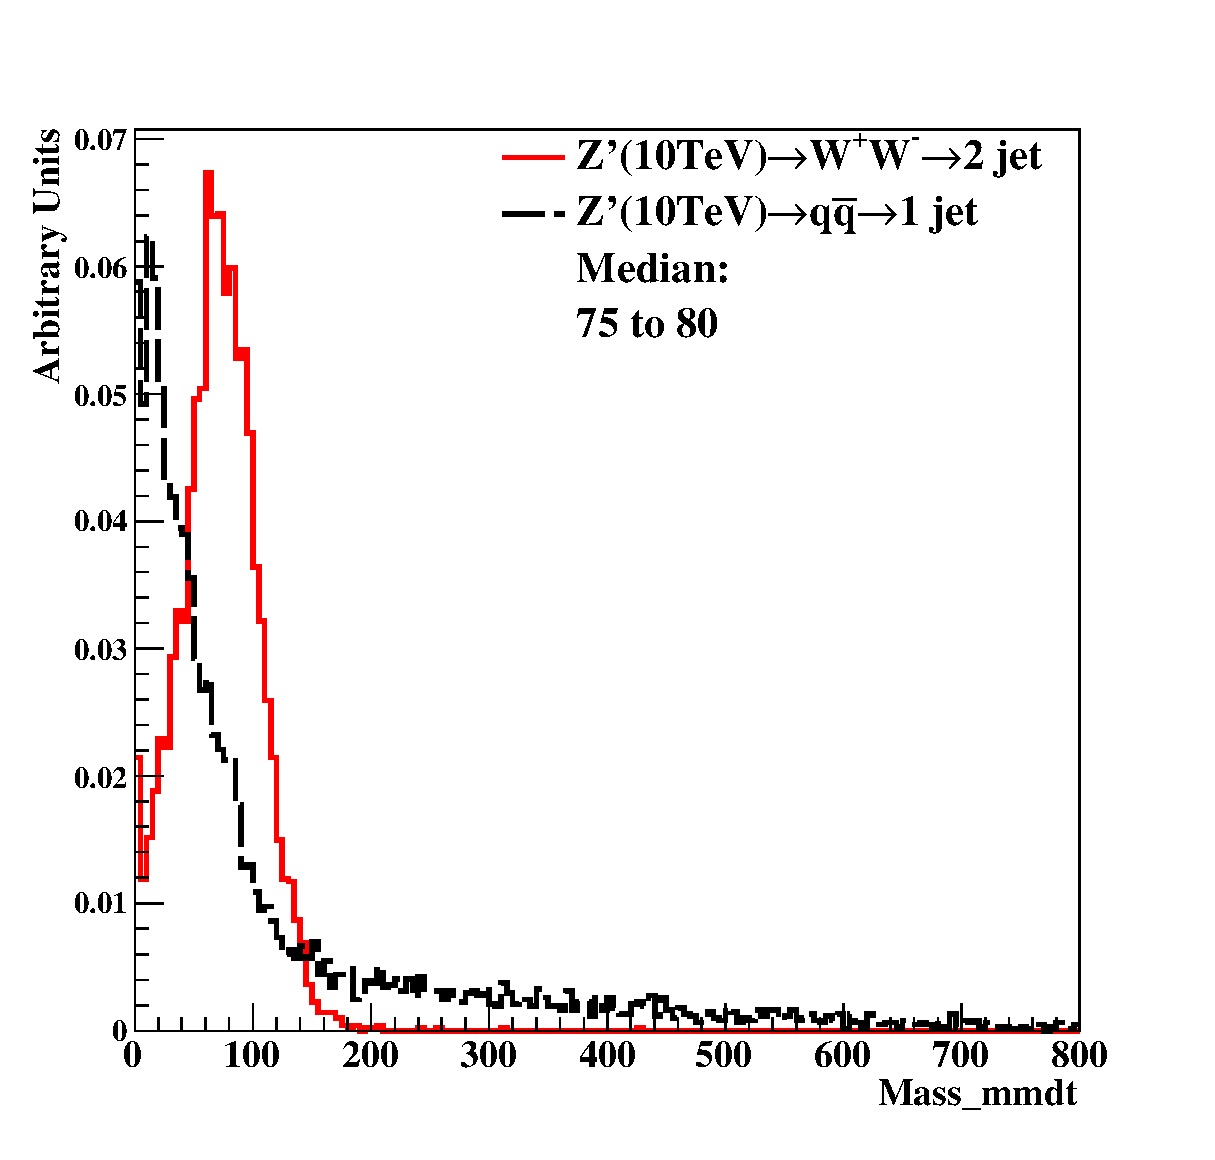
\includegraphics[width=0.22\textwidth]{figs/Dis_cluster_009_mass_mmdt_10tev_04.eps}
   }
      \subfigure[20TeV at 5$\times$5(cm$\times$cm) in cluster] {
   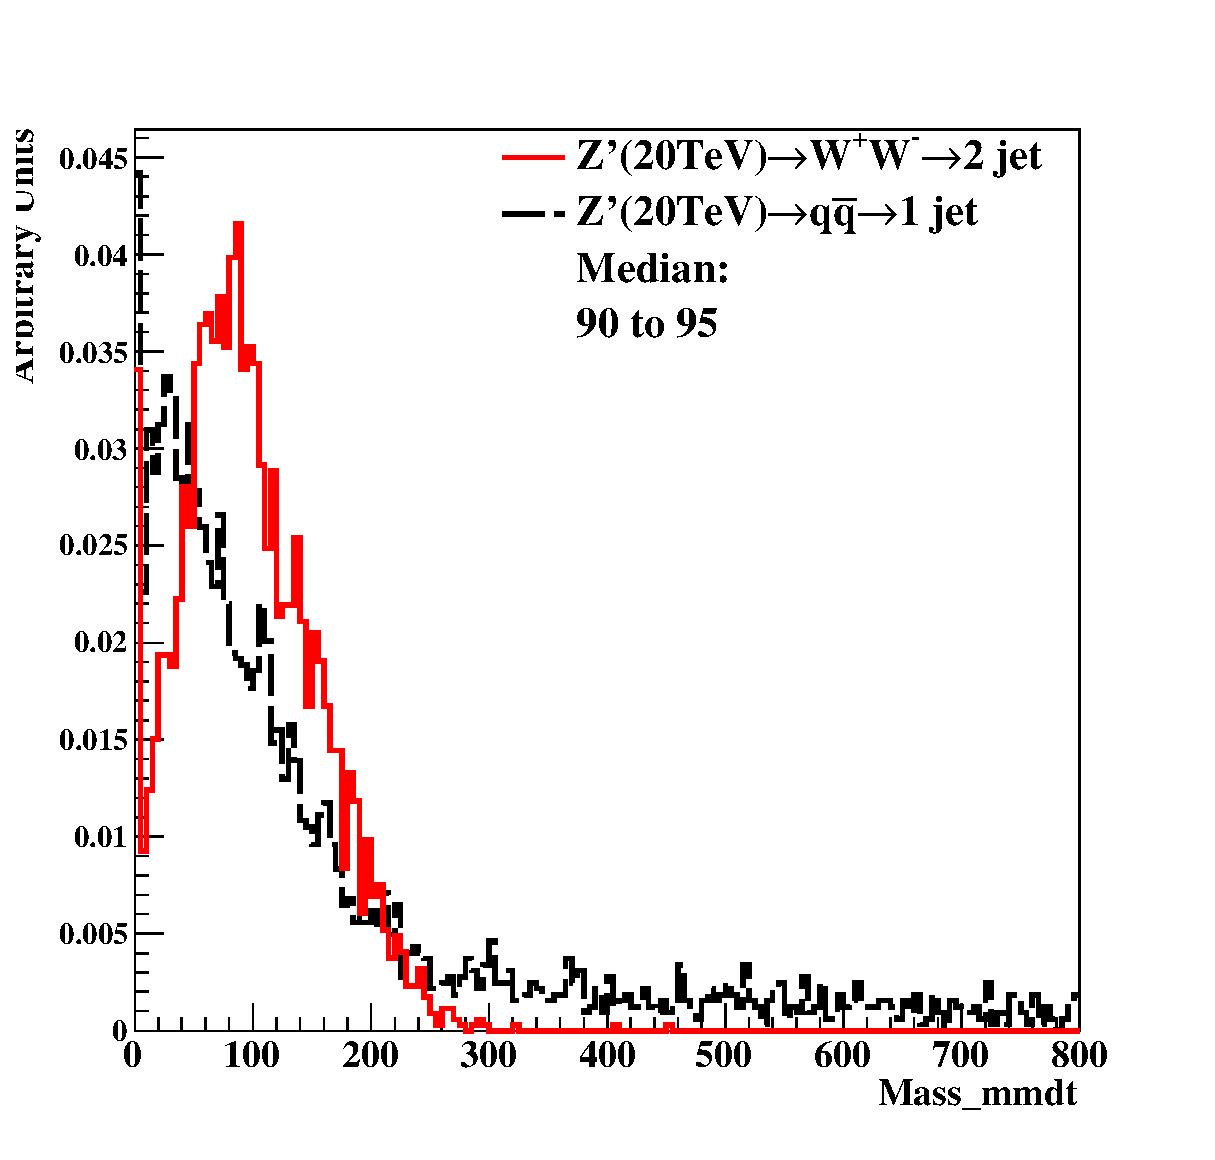
\includegraphics[width=0.22\textwidth]{figs/Dis_cluster_009_mass_mmdt_20tev_04.eps}\hfill
   }
      \subfigure[40TeV at 5$\times$5(cm$\times$cm) in cluster] {
   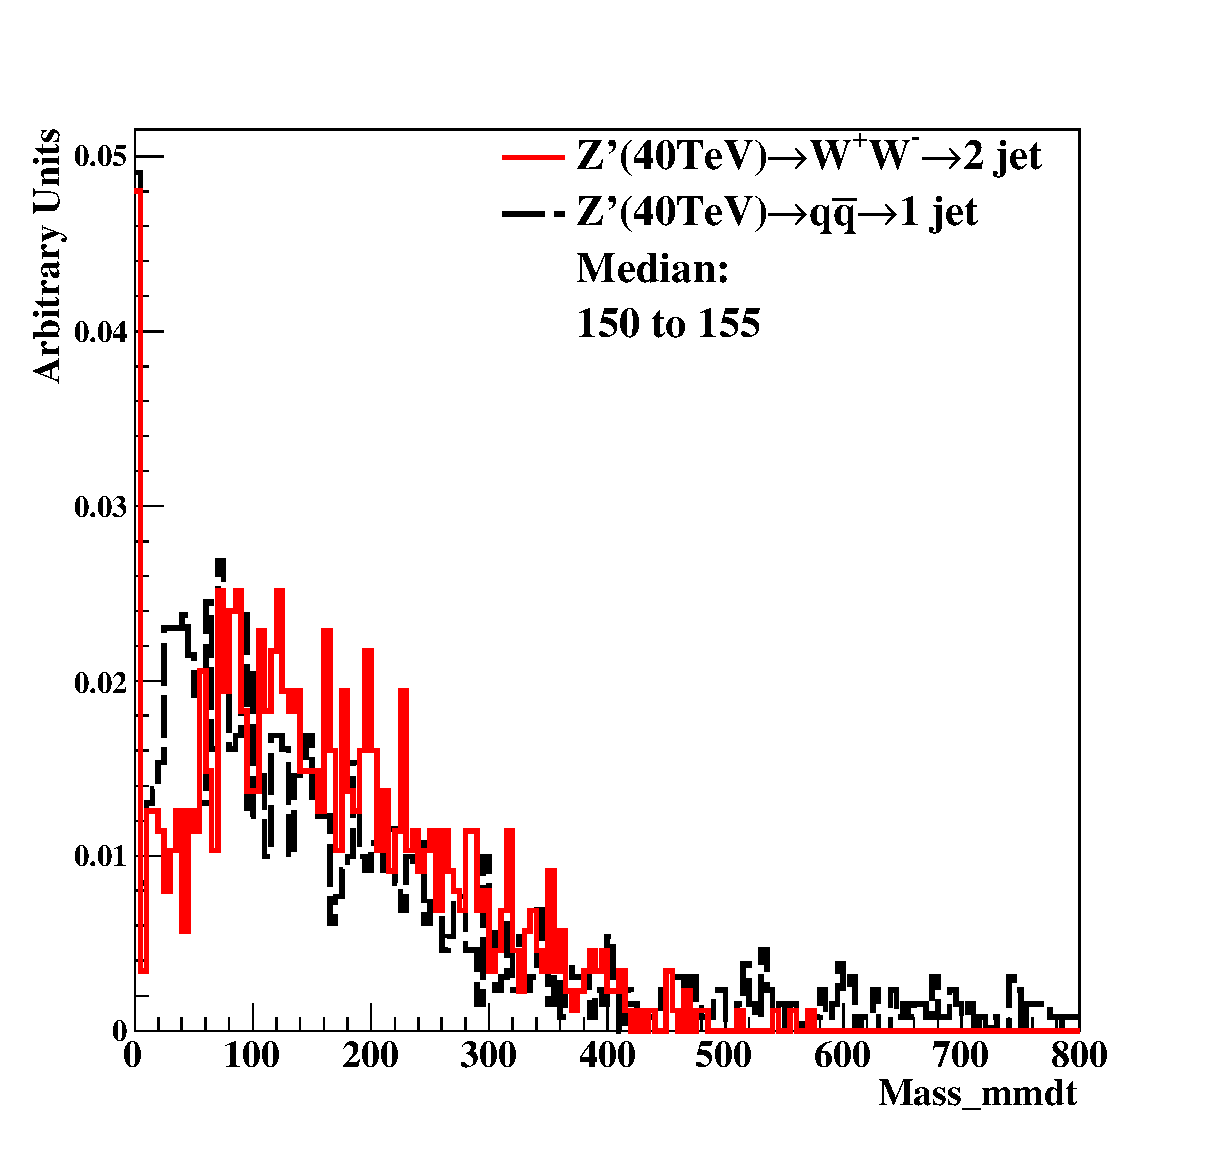
\includegraphics[width=0.22\textwidth]{figs/Dis_cluster_009_mass_mmdt_40tev_04.eps}\hfill
   }
   \subfigure[5TeV at 1$\times$1(cm$\times$cm) in cluster] {
   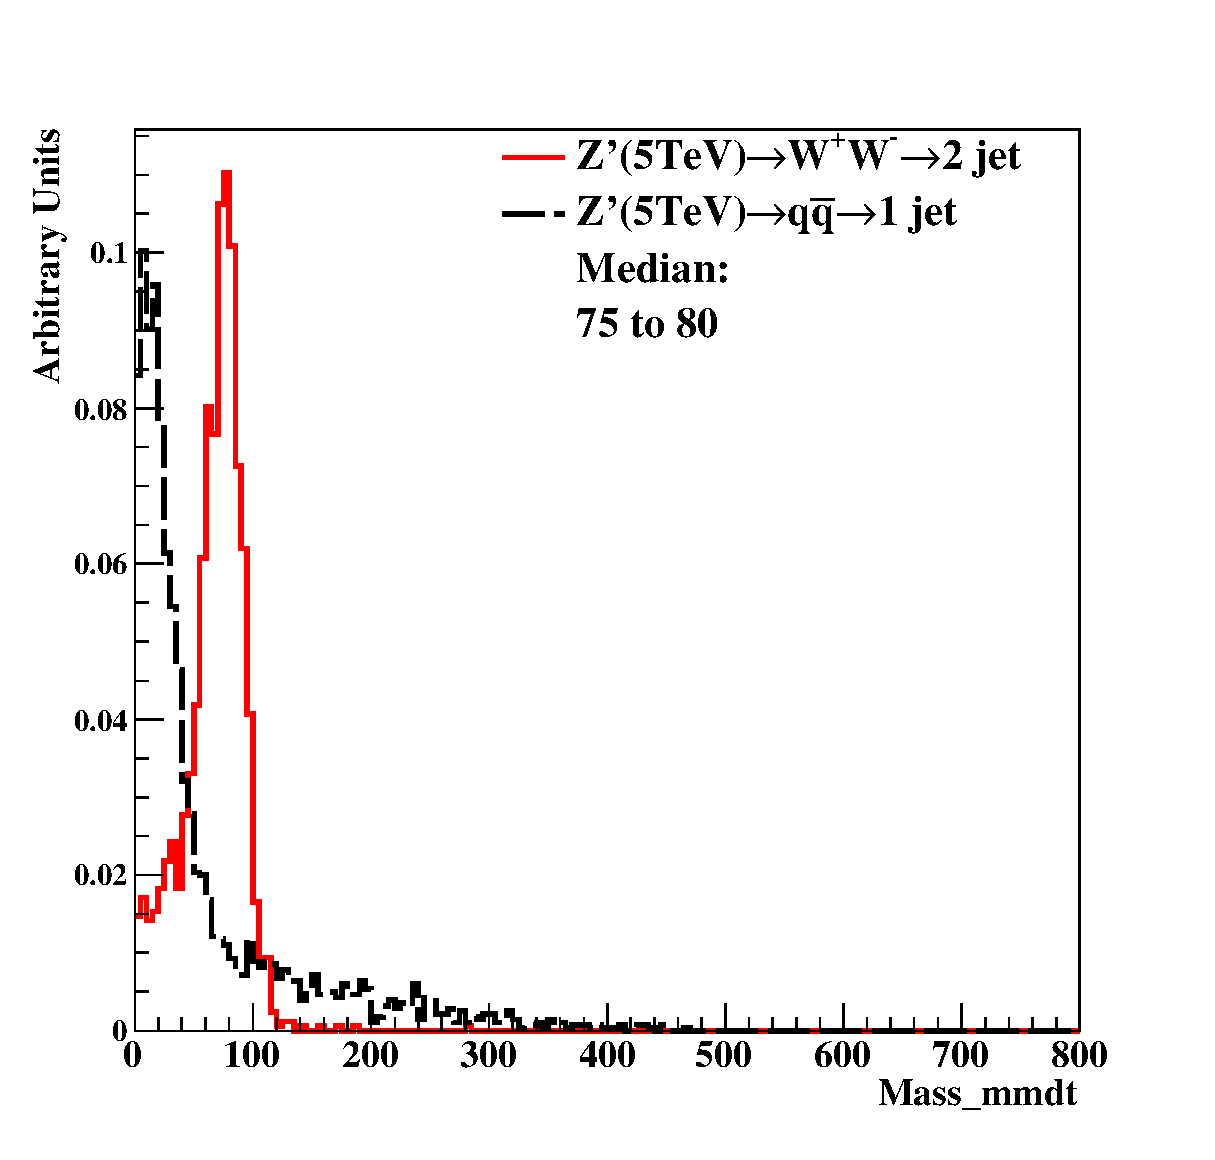
\includegraphics[width=0.22\textwidth]{figs/Dis_cluster_012_mass_mmdt_5tev_04.eps}\hfill
   }
    \subfigure[10TeV at 1$\times$1(cm$\times$cm) in cluster] {
   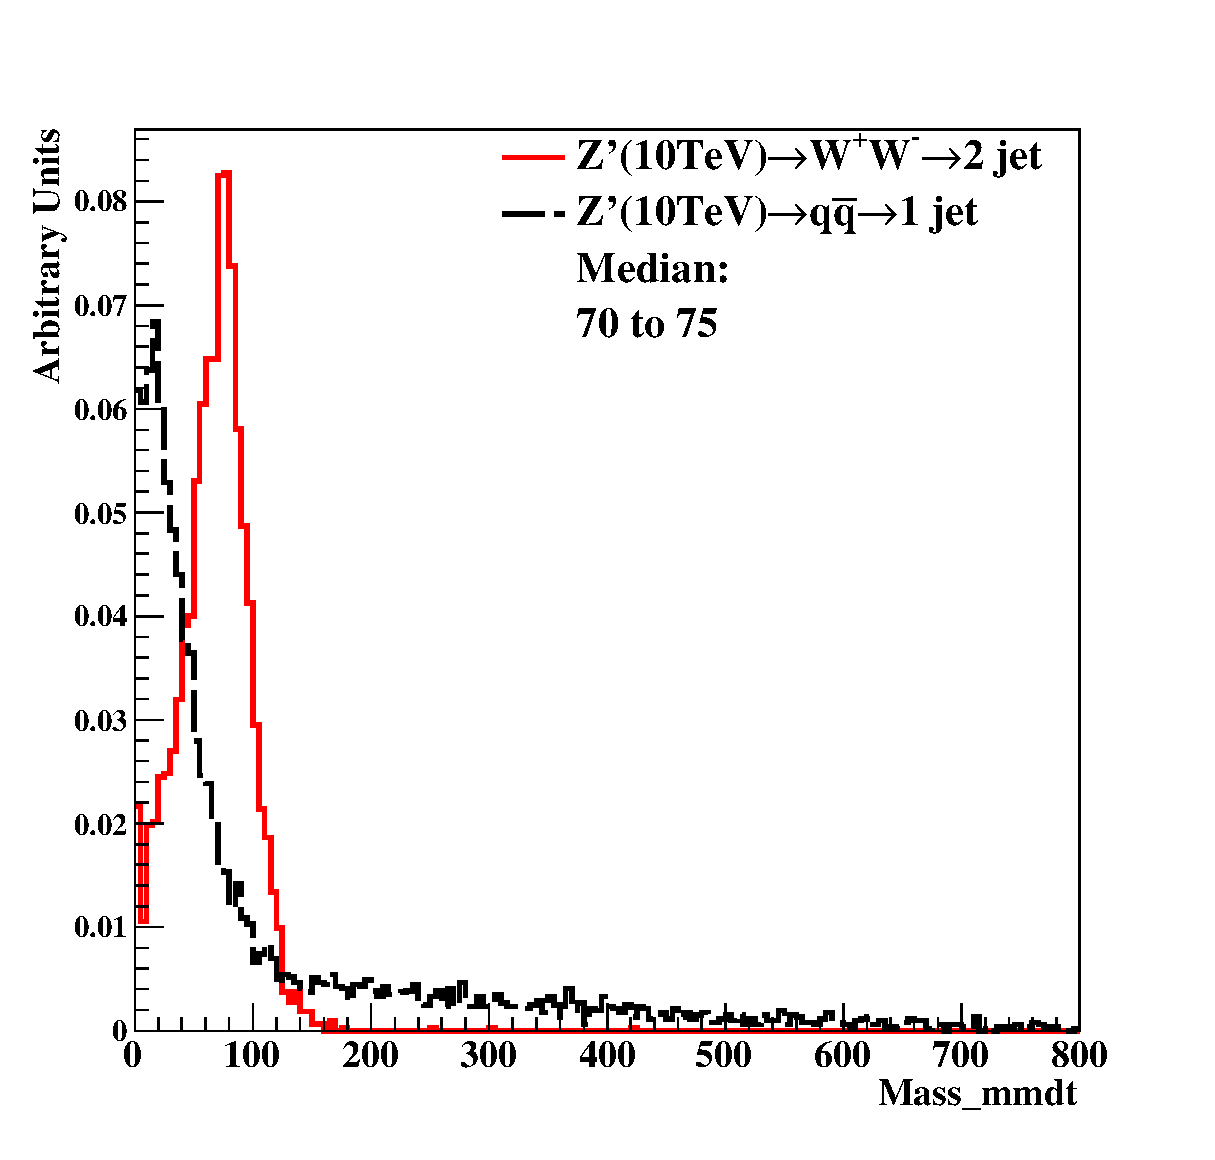
\includegraphics[width=0.22\textwidth]{figs/Dis_cluster_012_mass_mmdt_10tev_04.eps}
   }
   \subfigure[20TeV at 1$\times$1(cm$\times$cm) in cluster] {
   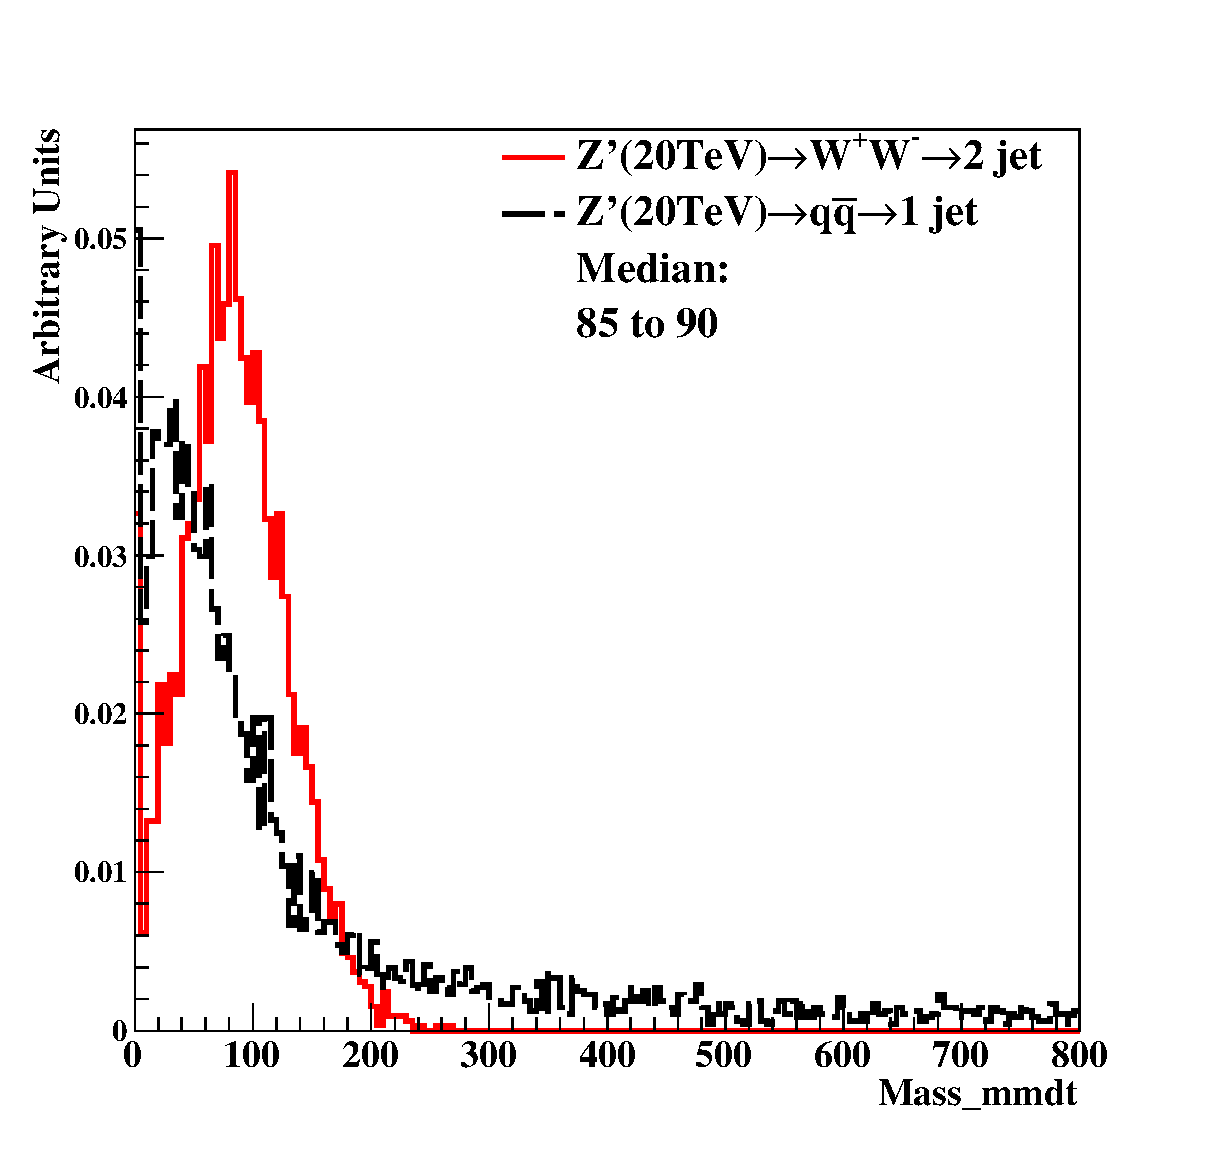
\includegraphics[width=0.22\textwidth]{figs/Dis_cluster_012_mass_mmdt_20tev_04.eps}\hfill
   }
      \subfigure[40TeV at 1$\times$1(cm$\times$cm) in cluster] {
   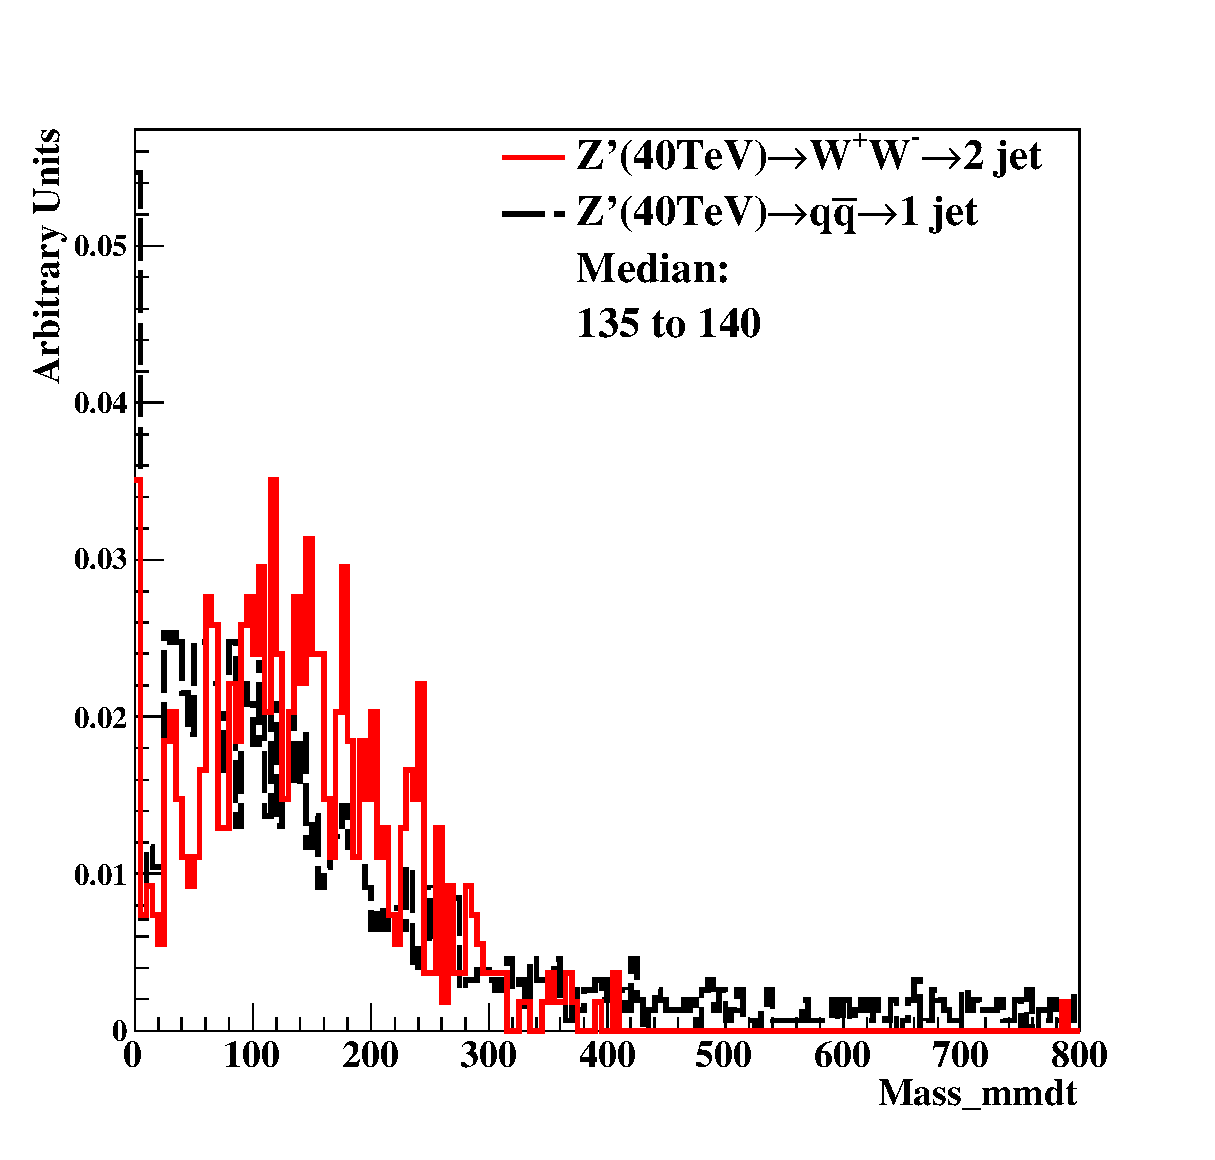
\includegraphics[width=0.22\textwidth]{figs/Dis_cluster_012_mass_mmdt_40tev_04.eps}
   }

\end{center}
\caption{Distributions of mass soft drop at $\beta$=0, signal=ww, in 5,10TeV energy of collision  in different detector sizes. Cell Size in 20$\times$20, 5$\times$5, and 1$\times$1(cm$\times$cm) are shown here.}
\label{fig:cluster_tau21_tau32}
\end{figure}

\begin{figure}
\begin{center}
  \subfigure[Central at Median($20\times20$=80,$5\times5$=80,$1\times1$=80) change width in cluster at 5TeV] {
  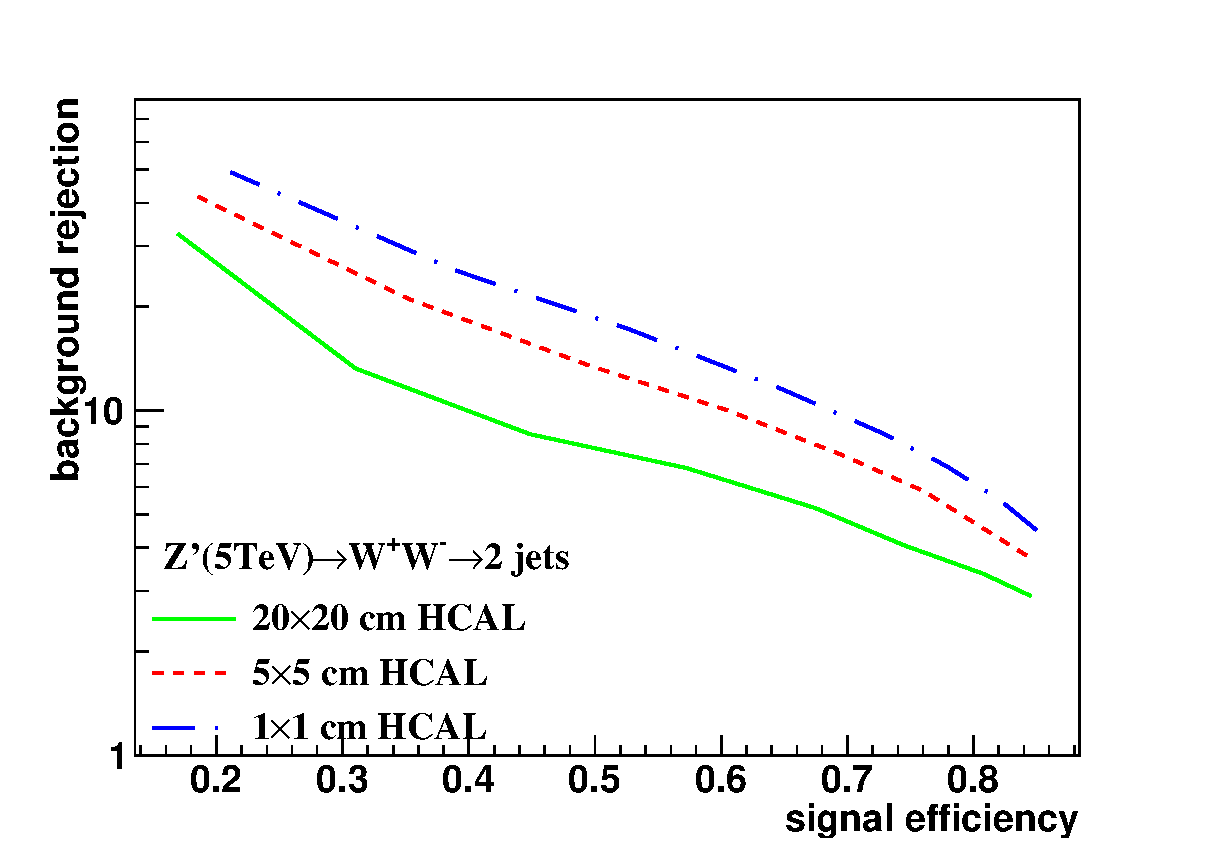
\includegraphics[width=0.43\textwidth]{figs/A_Cluster_mass_mmdt_5tev_eff_1_central_fix_ww_qq_log.eps}
  }
  \subfigure[Central at Median($20\times20$=95,$5\times5$=80,$1\times1$=75) change width in cluster at 10TeV] {
  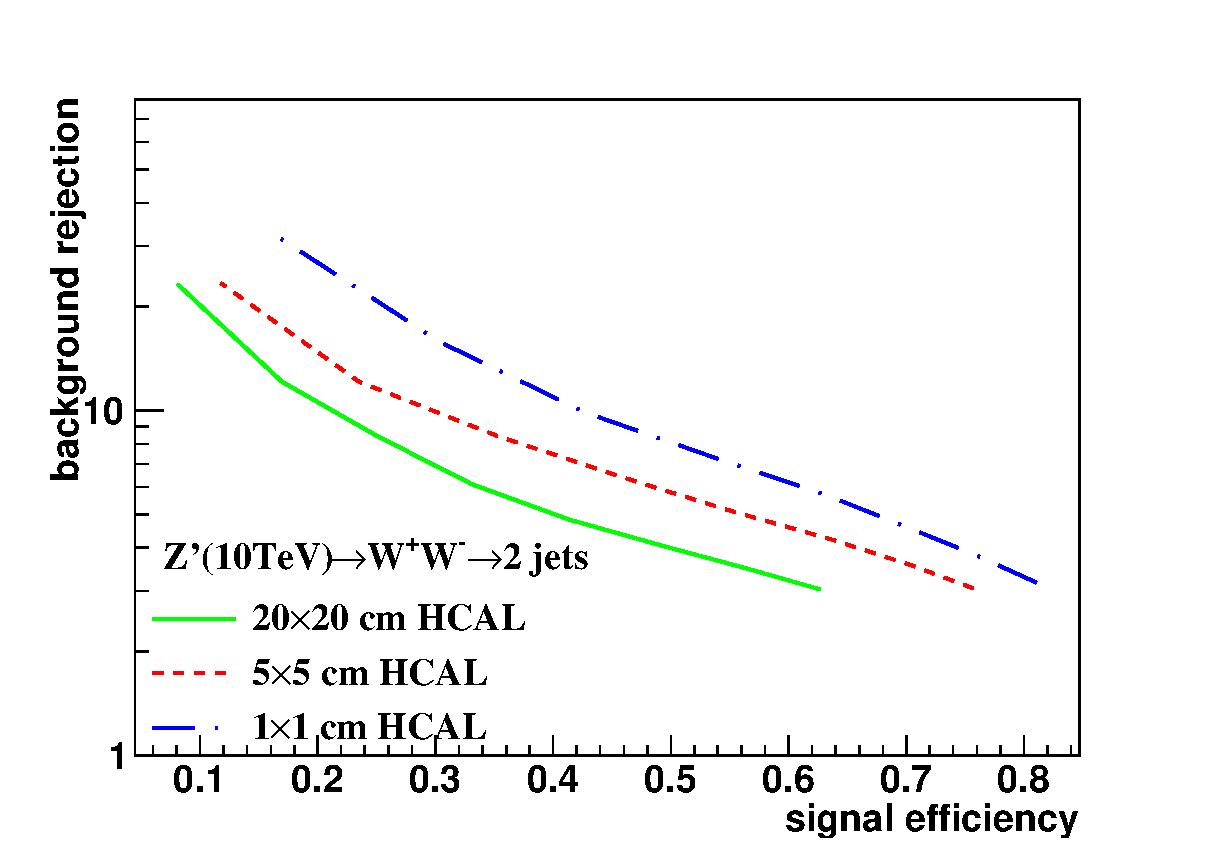
\includegraphics[width=0.43\textwidth]{figs/A_Cluster_mass_mmdt_10tev_eff_1_central_fix_ww_qq_log.eps}
  }
 \subfigure[Central at Median($20\times20$=155,$5\times5$=95,$1\times1$=90) change width in cluster at 20TeV] {
 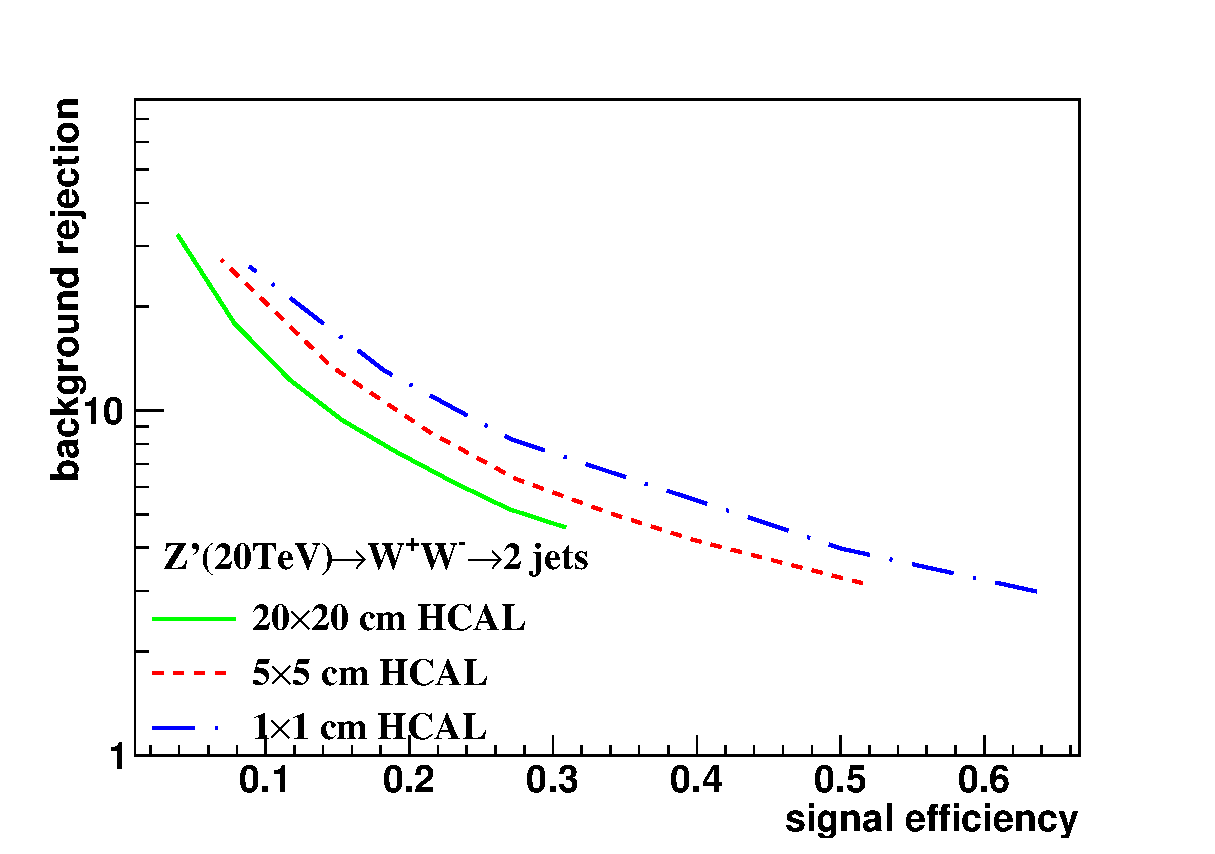
\includegraphics[width=0.43\textwidth]{figs/A_Cluster_mass_mmdt_20tev_eff_1_central_fix_ww_qq_log.eps}
 }
 \subfigure[Central at Median($20\times20$=130,$5\times5$=150,$1\times1$=135) change width in cluster at 40TeV] {
 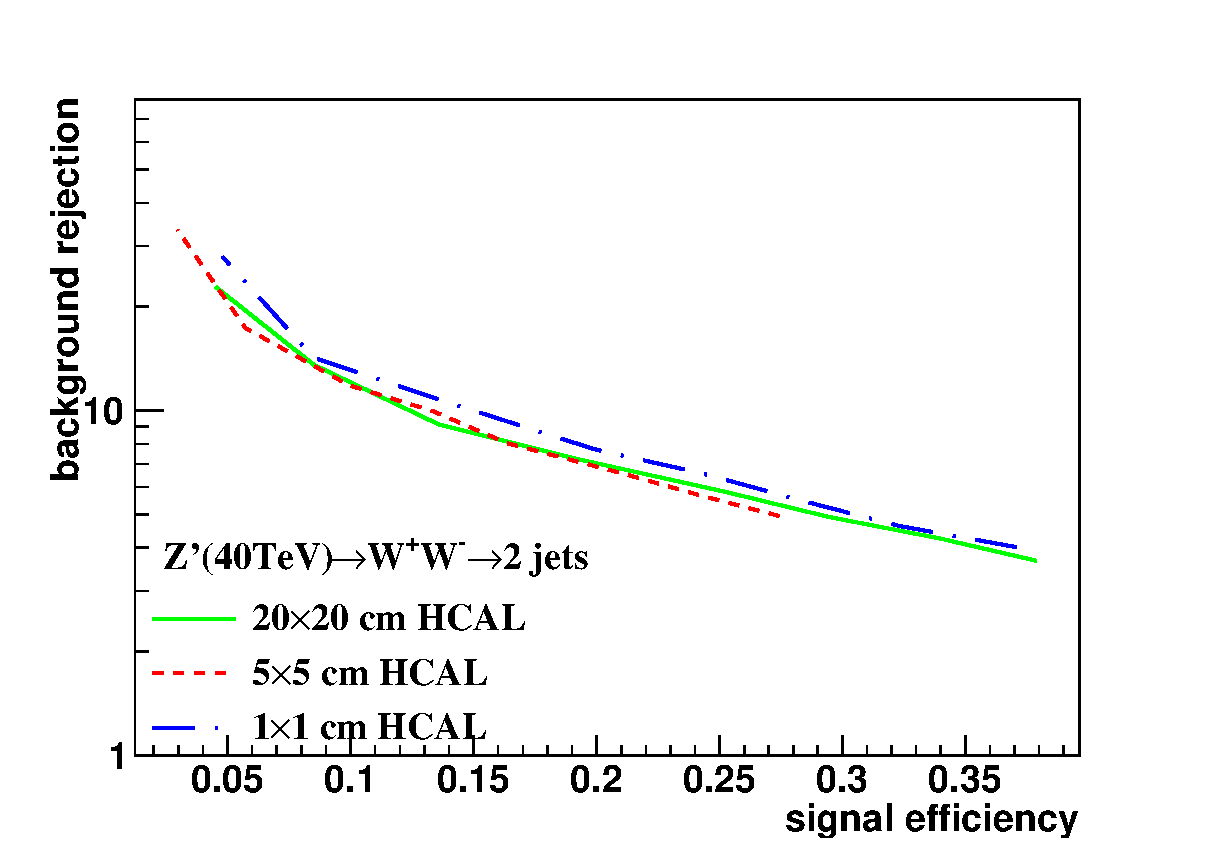
\includegraphics[width=0.43\textwidth]{figs/A_Cluster_mass_mmdt_40tev_eff_1_central_fix_ww_qq_log.eps}
 }
\end{center}
\caption{study of "fix central and change width" in mass soft drop at $\beta$=0, signal=ww, in 5, 10, 20, 40TeV energy of collision  in different detector sizes. Cell Size in 20$\times$20, 5$\times$5, and 1$\times$1(cm$\times$cm) are shown in each picture.}
\label{fig:cluster_tau21_tau32}
\end{figure}

\begin{figure}
\begin{center}
   \subfigure[5TeV at 20$\times$20(cm$\times$cm) in cluster] {
   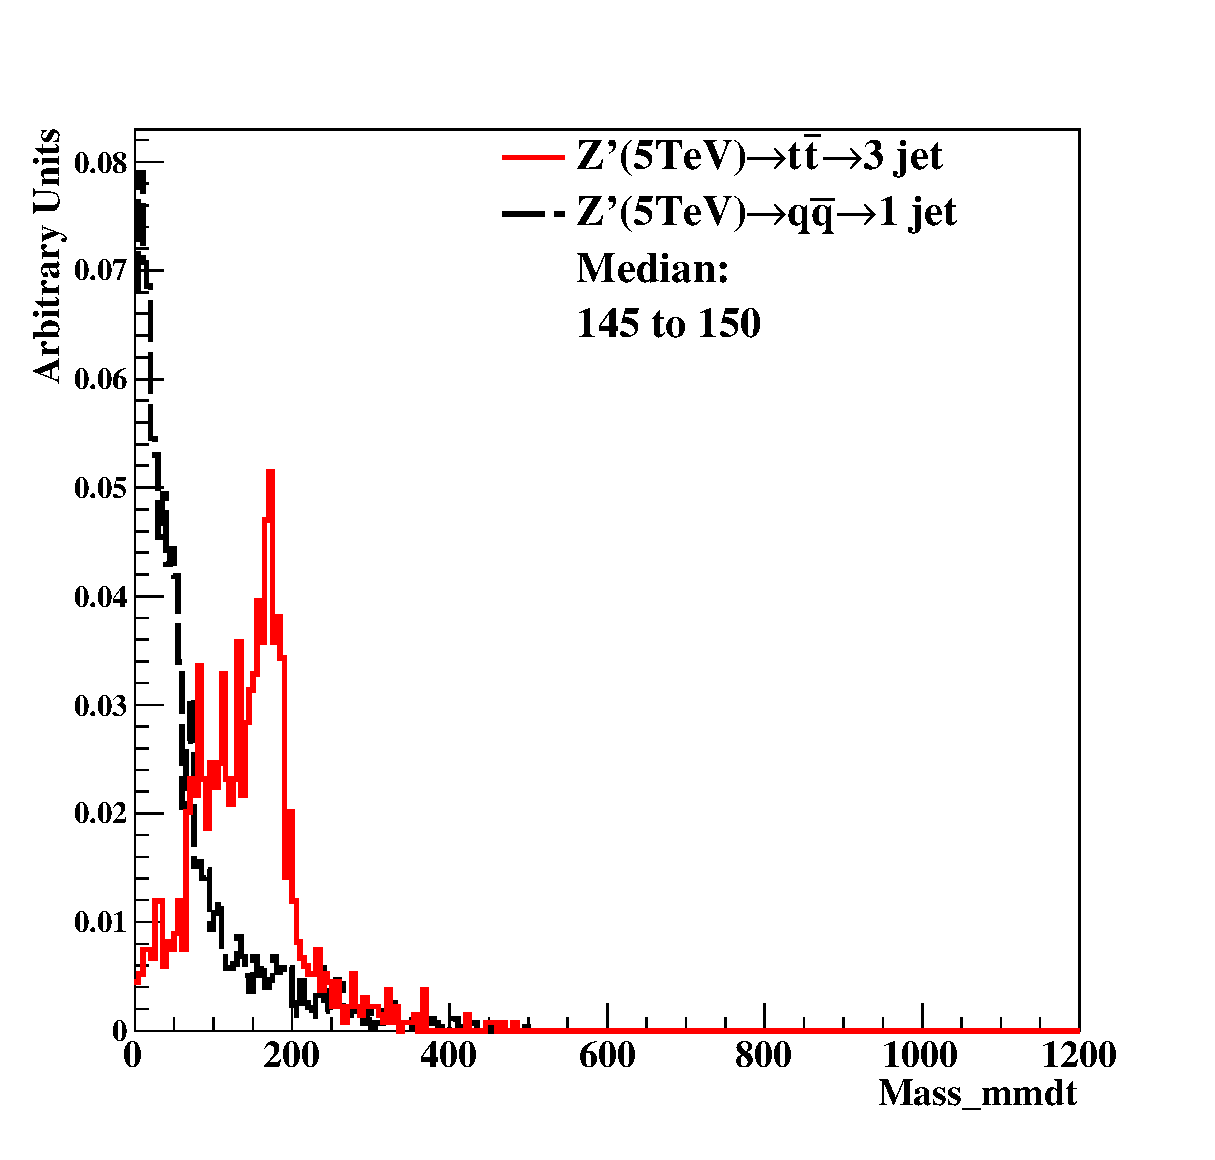
\includegraphics[width=0.22\textwidth]{figs/Dis_cluster_010_mass_mmdt_tt_5tev_04_tt.eps}
   }
      \subfigure[10TeV at 20$\times$20(cm$\times$cm) in cluster] {
   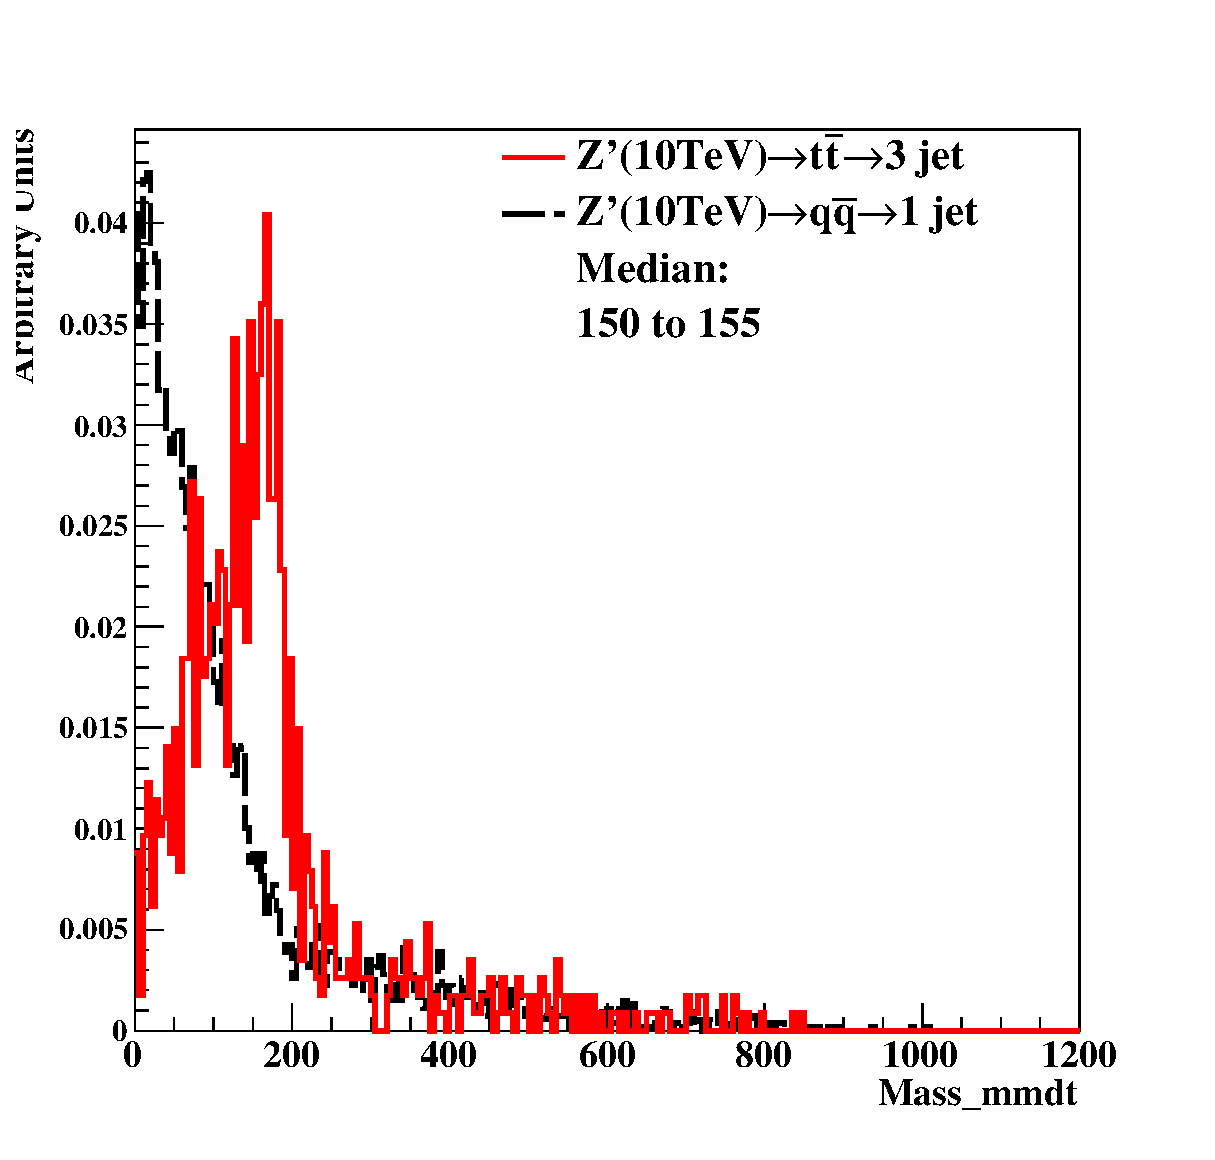
\includegraphics[width=0.22\textwidth]{figs/Dis_cluster_010_mass_mmdt_tt_10tev_04_tt.eps}
   }
   \subfigure[20TeV at 5$\times$5(cm$\times$cm) in cluster] {
   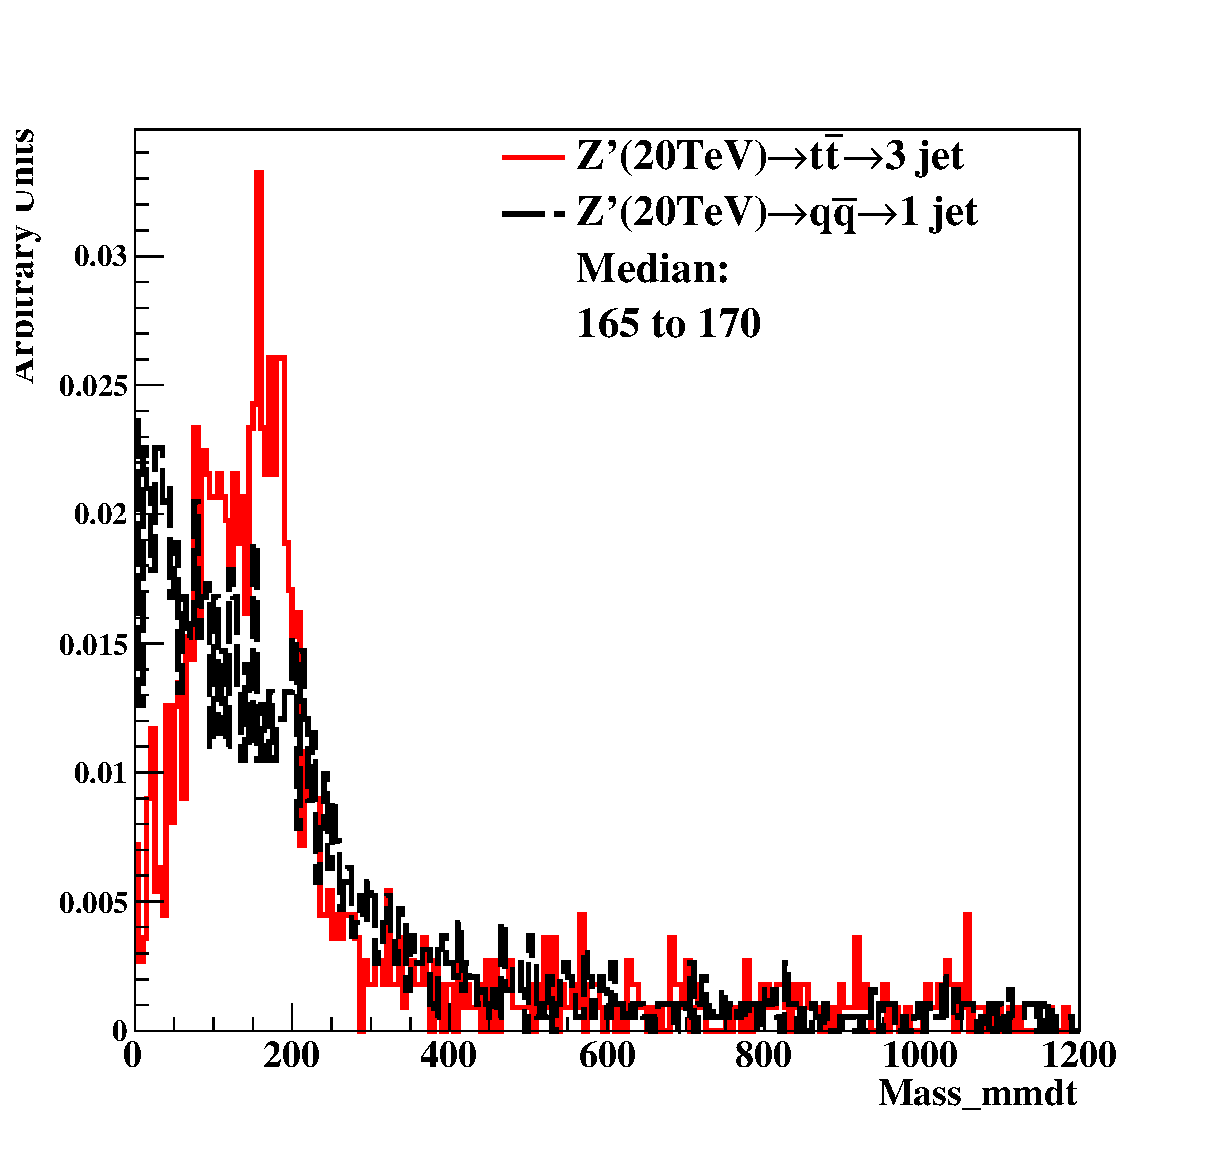
\includegraphics[width=0.22\textwidth]{figs/Dis_cluster_010_mass_mmdt_tt_20tev_04_tt.eps}
   }
    \subfigure[40TeV at 5$\times$5(cm$\times$cm) in cluster] {
   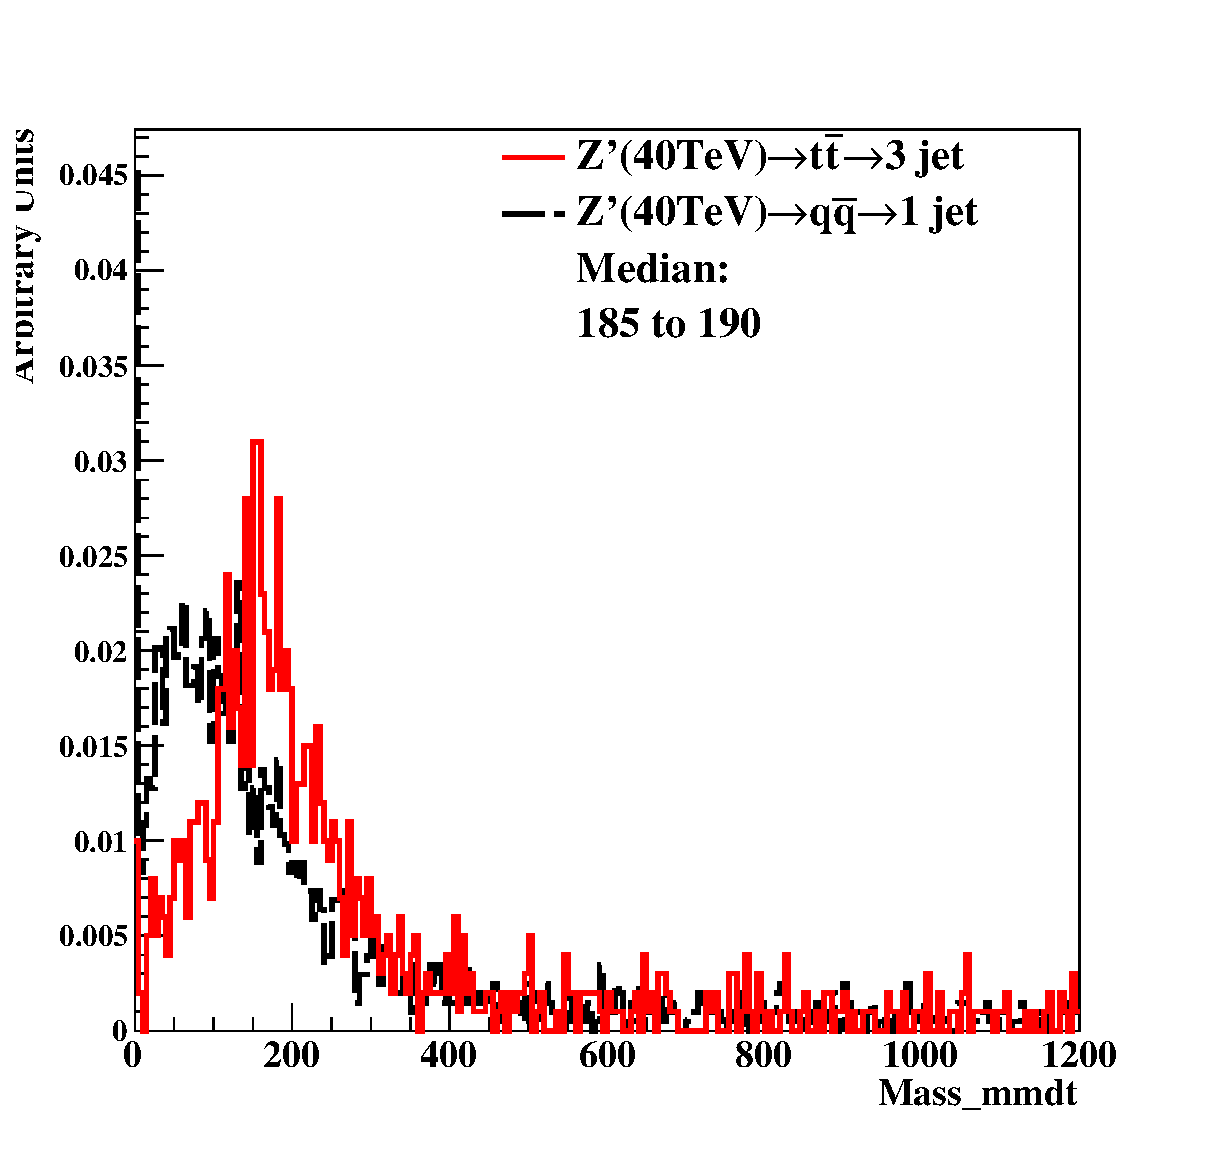
\includegraphics[width=0.22\textwidth]{figs/Dis_cluster_010_mass_mmdt_tt_40tev_04_tt.eps}
   }
   \subfigure[5TeV at 1$\times$1(cm$\times$cm) in cluster] {
   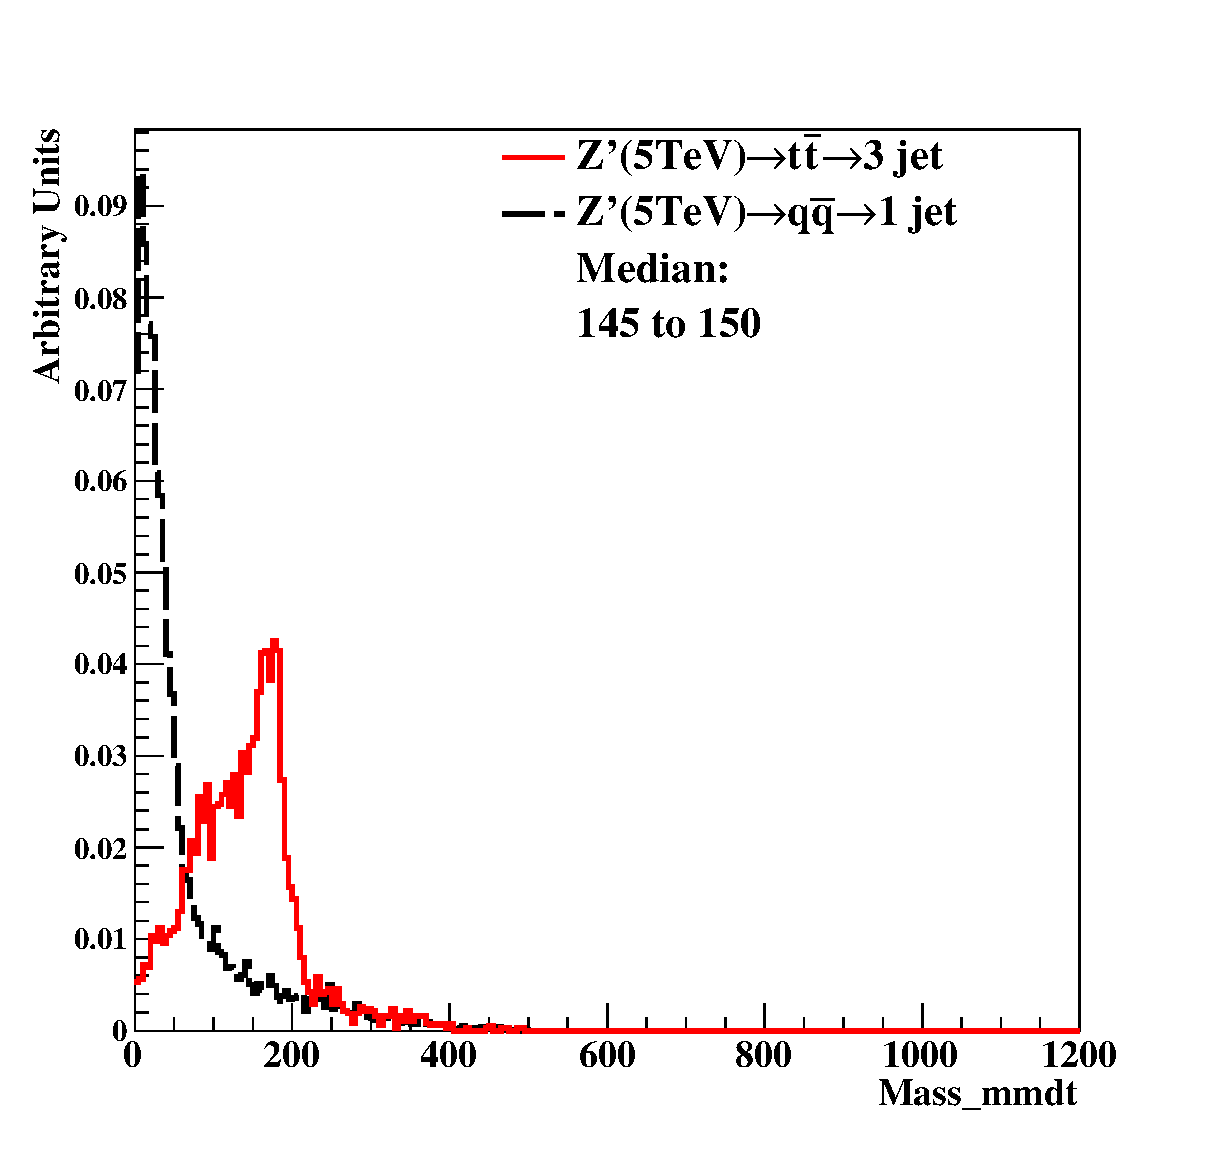
\includegraphics[width=0.22\textwidth]{figs/Dis_cluster_009_mass_mmdt_tt_5tev_04_tt.eps}
   }
   \subfigure[10TeV at 1$\times$1(cm$\times$cm) in cluster] {
   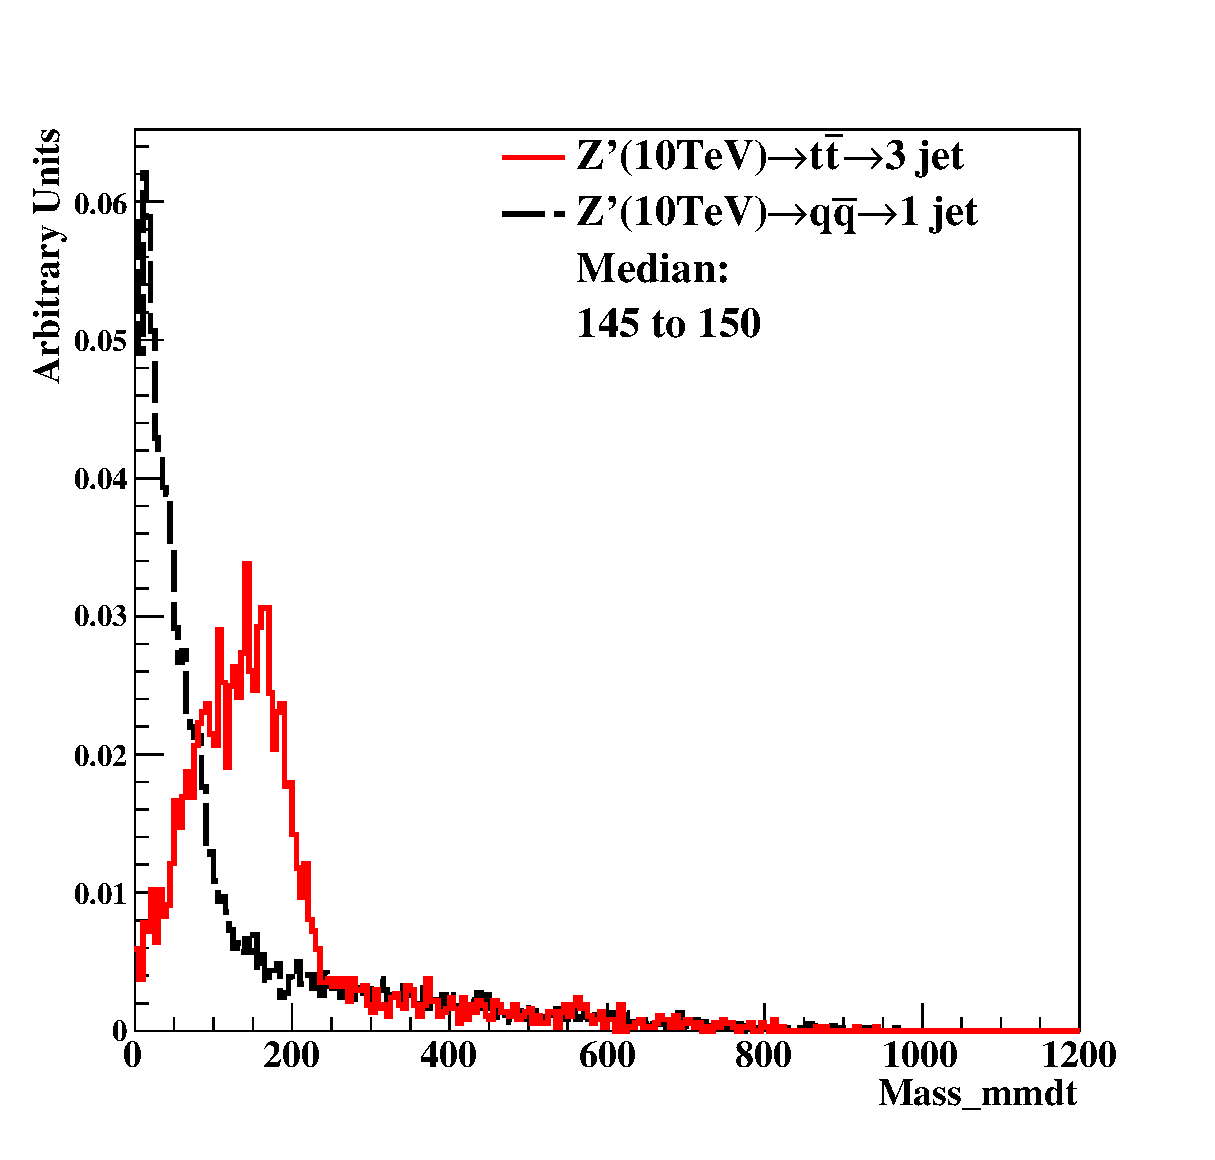
\includegraphics[width=0.22\textwidth]{figs/Dis_cluster_009_mass_mmdt_tt_10tev_04_tt.eps}
   }
   \subfigure[20TeV at 20$\times$20(cm$\times$cm) in cluster] {
   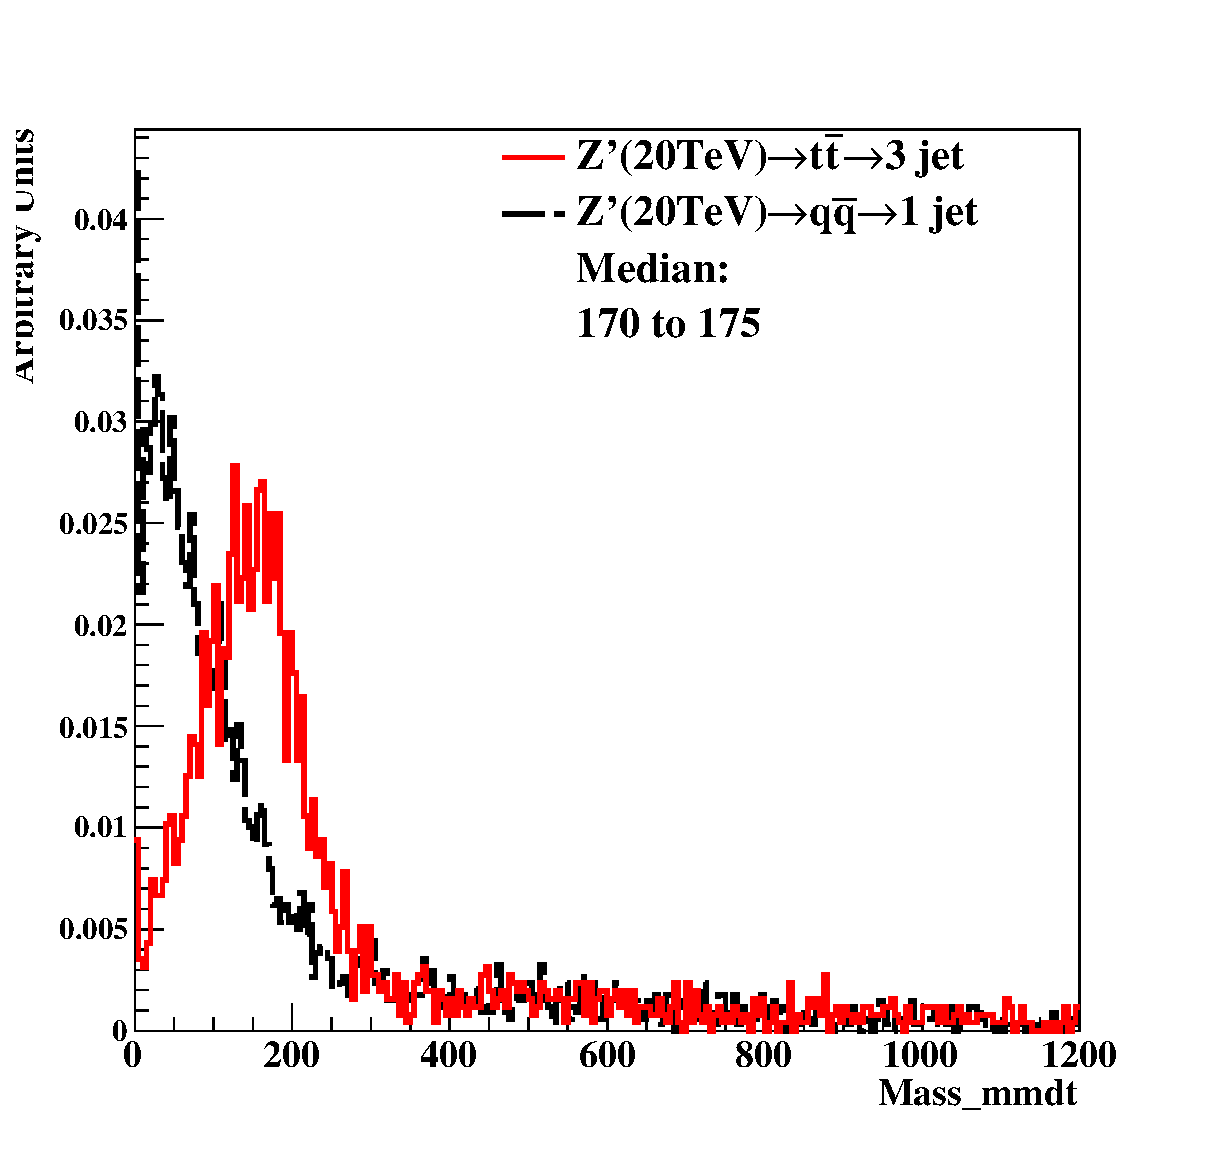
\includegraphics[width=0.22\textwidth]{figs/Dis_cluster_009_mass_mmdt_tt_20tev_04_tt.eps}\hfill
   }
      \subfigure[40TeV at 20$\times$20(cm$\times$cm) in cluster] {
   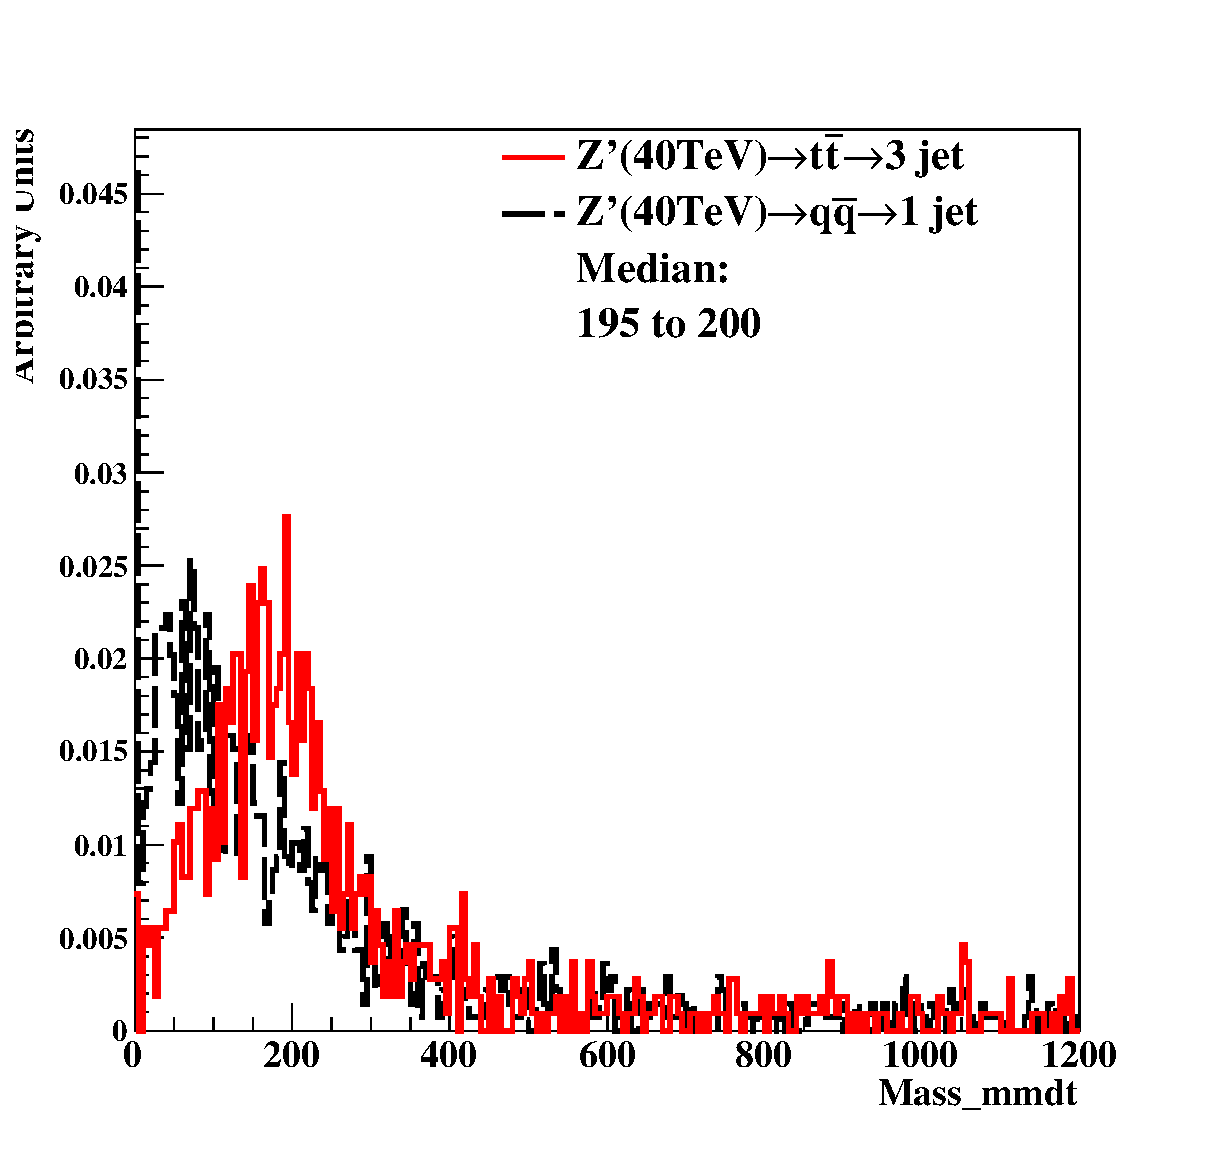
\includegraphics[width=0.22\textwidth]{figs/Dis_cluster_009_mass_mmdt_tt_40tev_04_tt.eps}\hfill
   }
   \subfigure[5TeV at 5$\times$5(cm$\times$cm) in cluster] {
   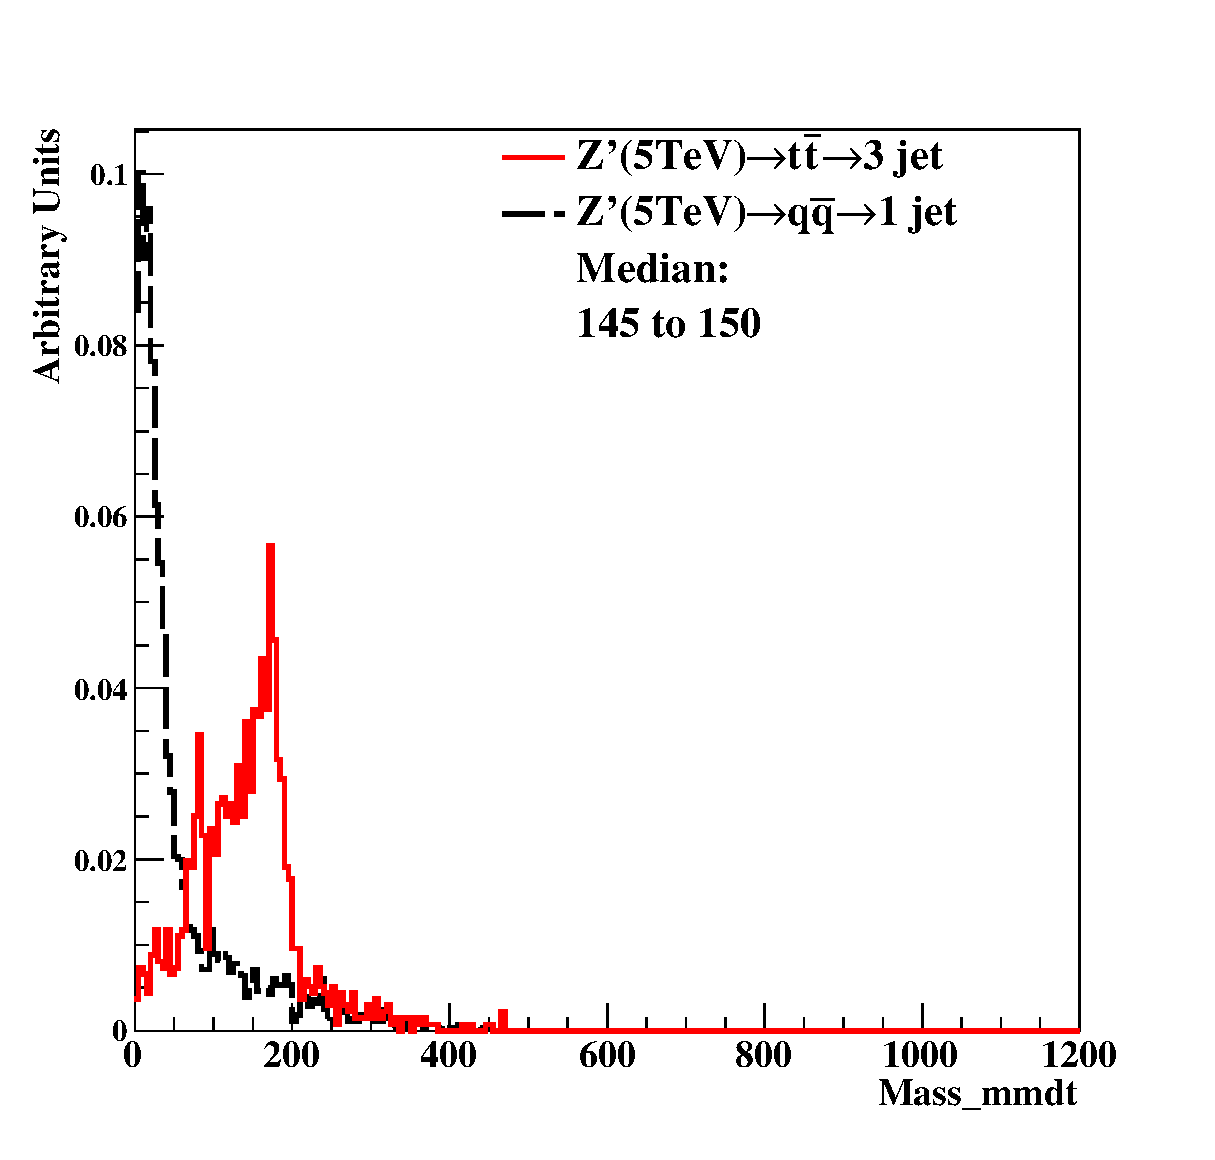
\includegraphics[width=0.22\textwidth]{figs/Dis_cluster_012_mass_mmdt_tt_5tev_04_tt.eps}\hfill
   }
    \subfigure[10TeV at 5$\times$5(cm$\times$cm) in cluster] {
   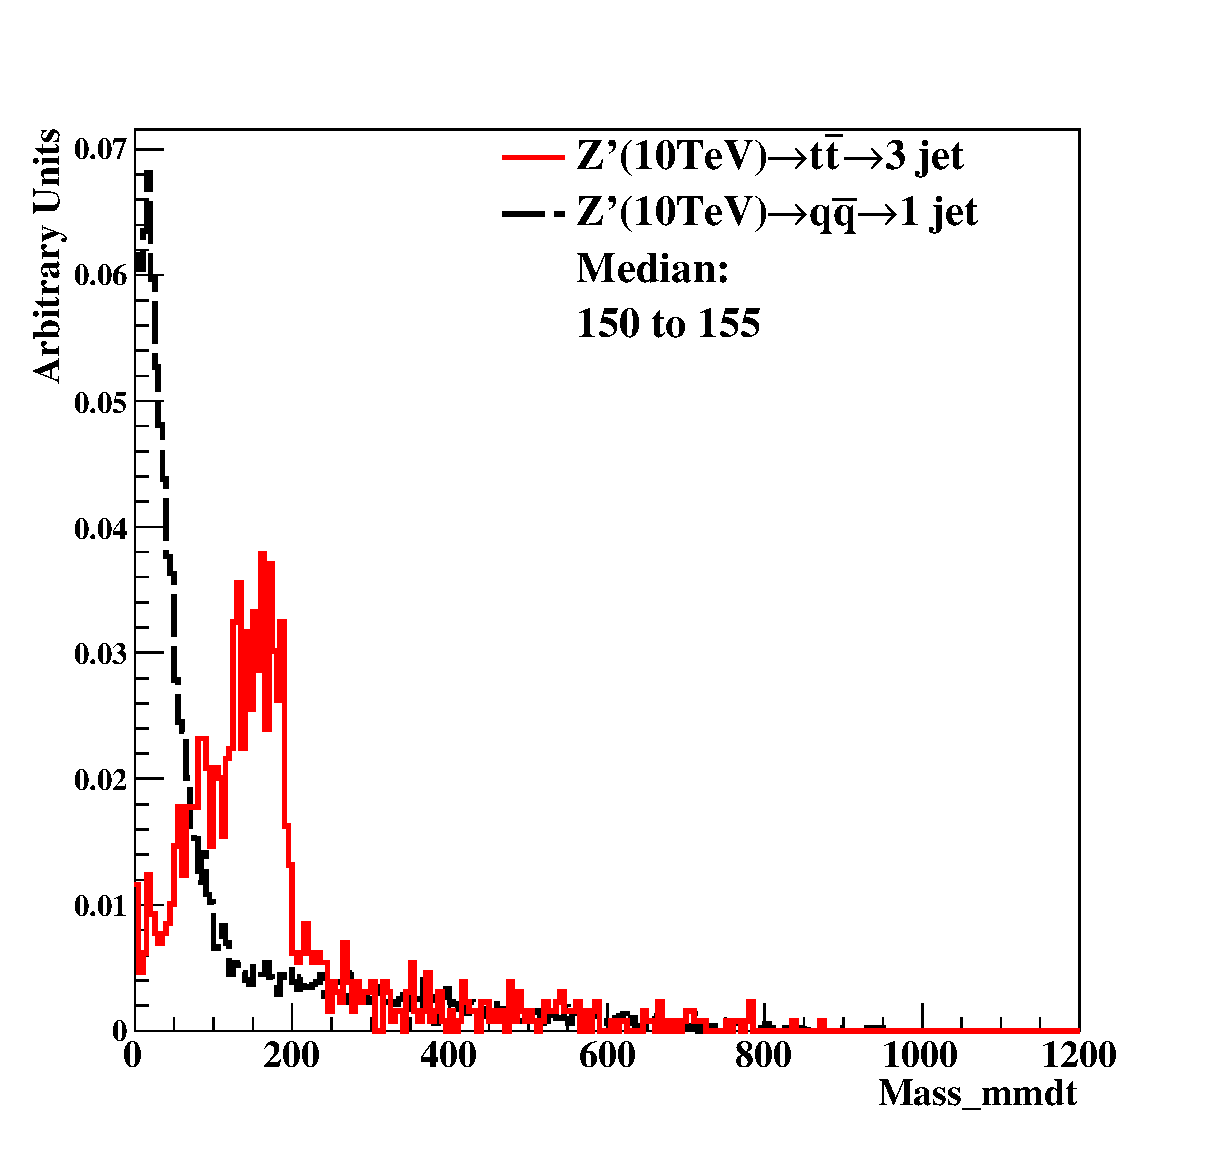
\includegraphics[width=0.22\textwidth]{figs/Dis_cluster_012_mass_mmdt_tt_10tev_04_tt.eps}
   }
   \subfigure[20TeV at 1$\times$1(cm$\times$cm) in cluster] {
   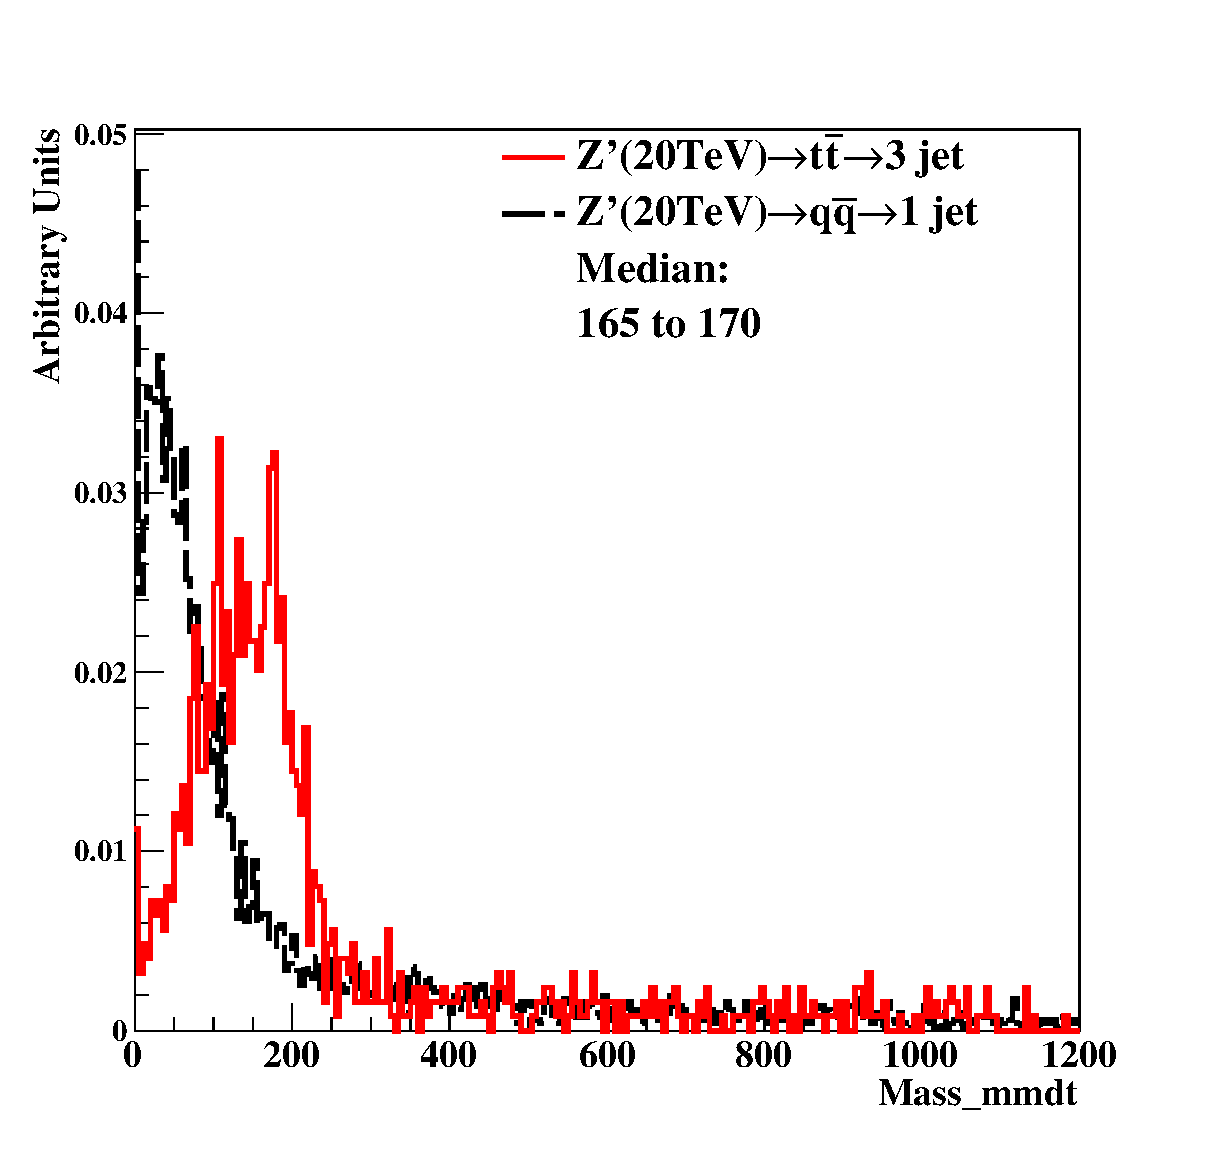
\includegraphics[width=0.22\textwidth]{figs/Dis_cluster_012_mass_mmdt_tt_20tev_04_tt.eps}\hfill
   }
      \subfigure[40TeV at 1$\times$1(cm$\times$cm) in cluster] {
   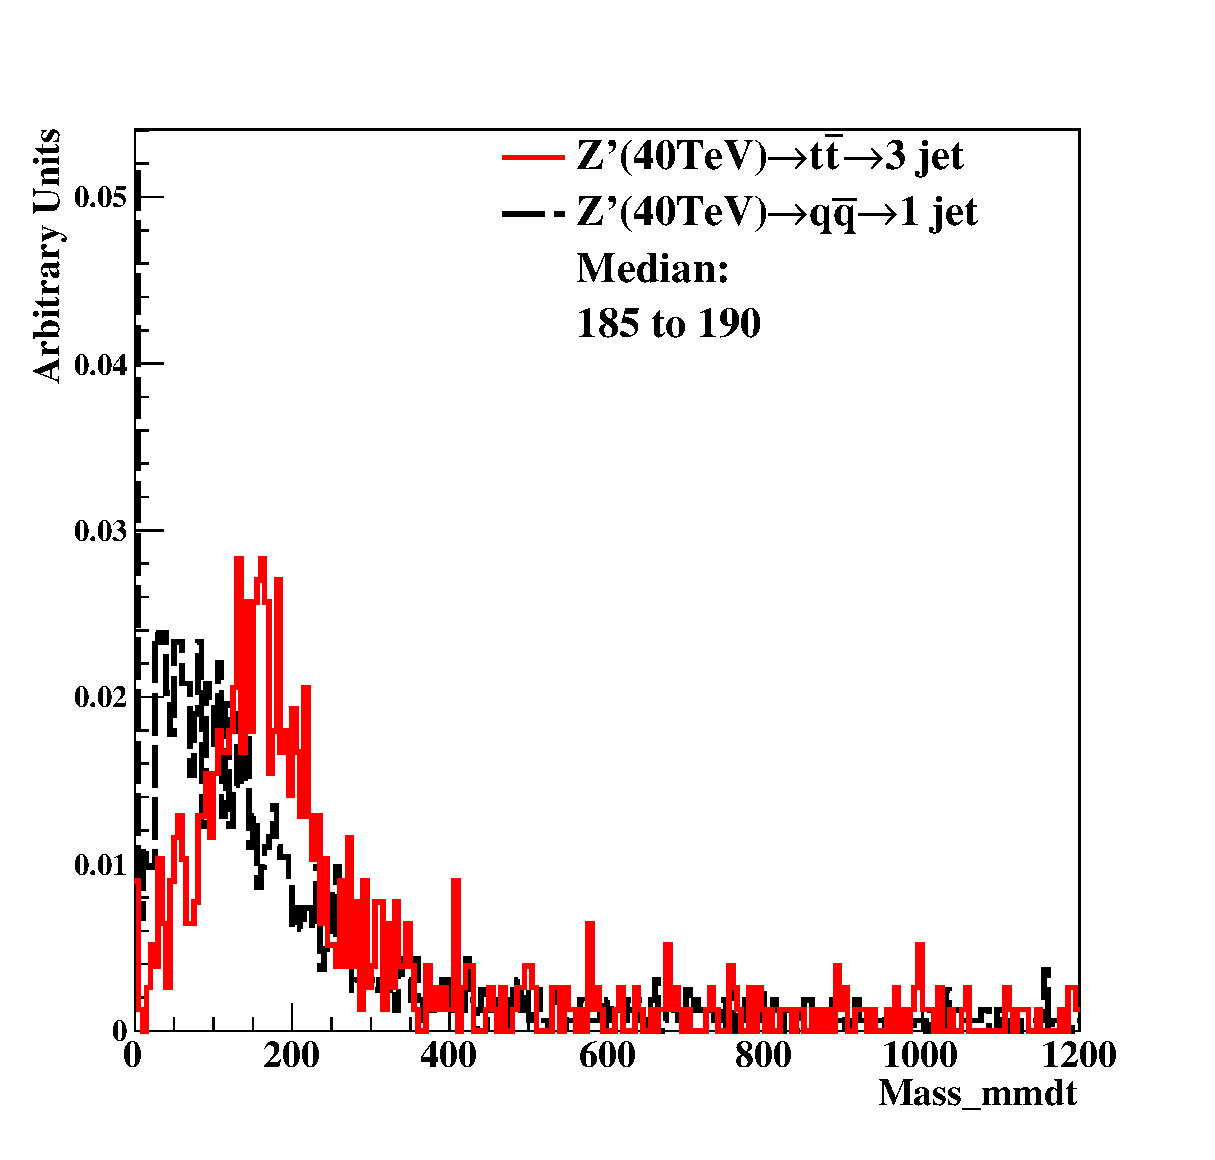
\includegraphics[width=0.22\textwidth]{figs/Dis_cluster_012_mass_mmdt_tt_40tev_04_tt.eps}
   }
\end{center}
\caption{Distributions of mass soft drop at $\beta$=0, signal=tt, in 5,10TeV energy of collision  in different detector sizes. Cell Size in 20$\times$20, 5$\times$5, and 1$\times$1(cm$\times$cm) are shown here.}
\label{fig:cluster_tau21_tau32}
\end{figure}

\begin{figure}
\begin{center}
  \subfigure[Central at Median($20\times20$=150,$5\times5$=150,$1\times1$=150) change width in cluster at 5TeV] {
  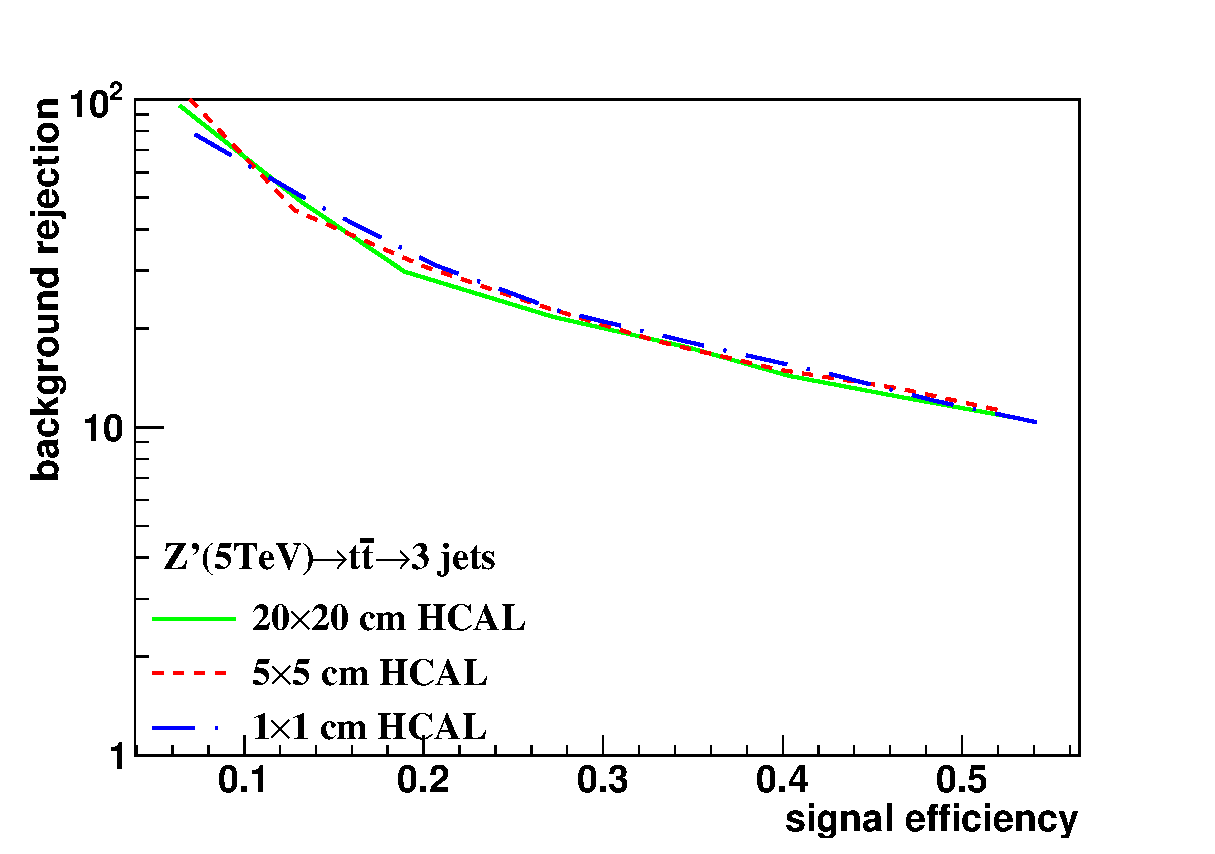
\includegraphics[width=0.43\textwidth]{figs/A_Cluster_mass_mmdt_5tev_eff_1_central_fix_tt_qq_log.eps}
  }
  \subfigure[Central at Median($20\times20$=155,$5\times5$=150,$1\times1$=155) change width in cluster at 10TeV] {
  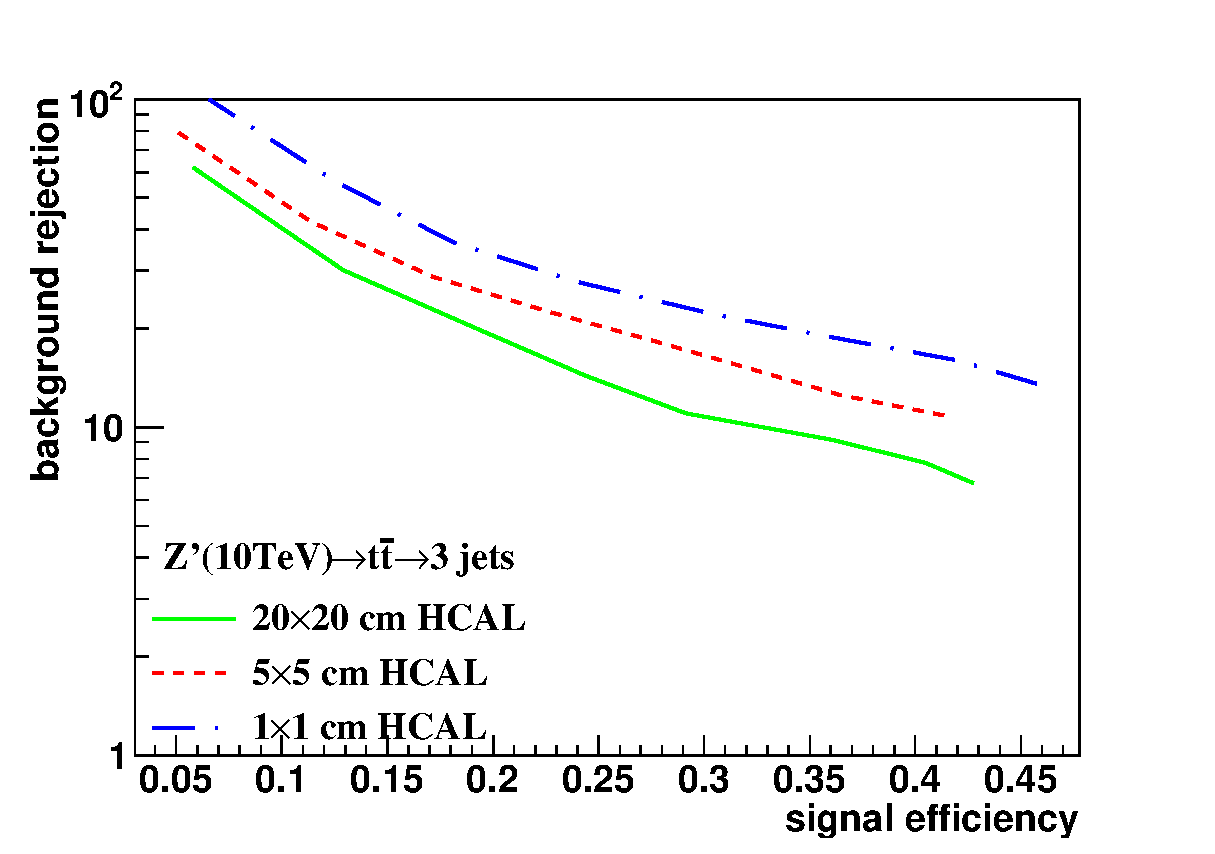
\includegraphics[width=0.43\textwidth]{figs/A_Cluster_mass_mmdt_10tev_eff_1_central_fix_tt_qq_log.eps}
  }
 \subfigure[Central at Median($20\times20$=165,$5\times5$=175,$1\times1$=170) change width in cluster at 20TeV] {
 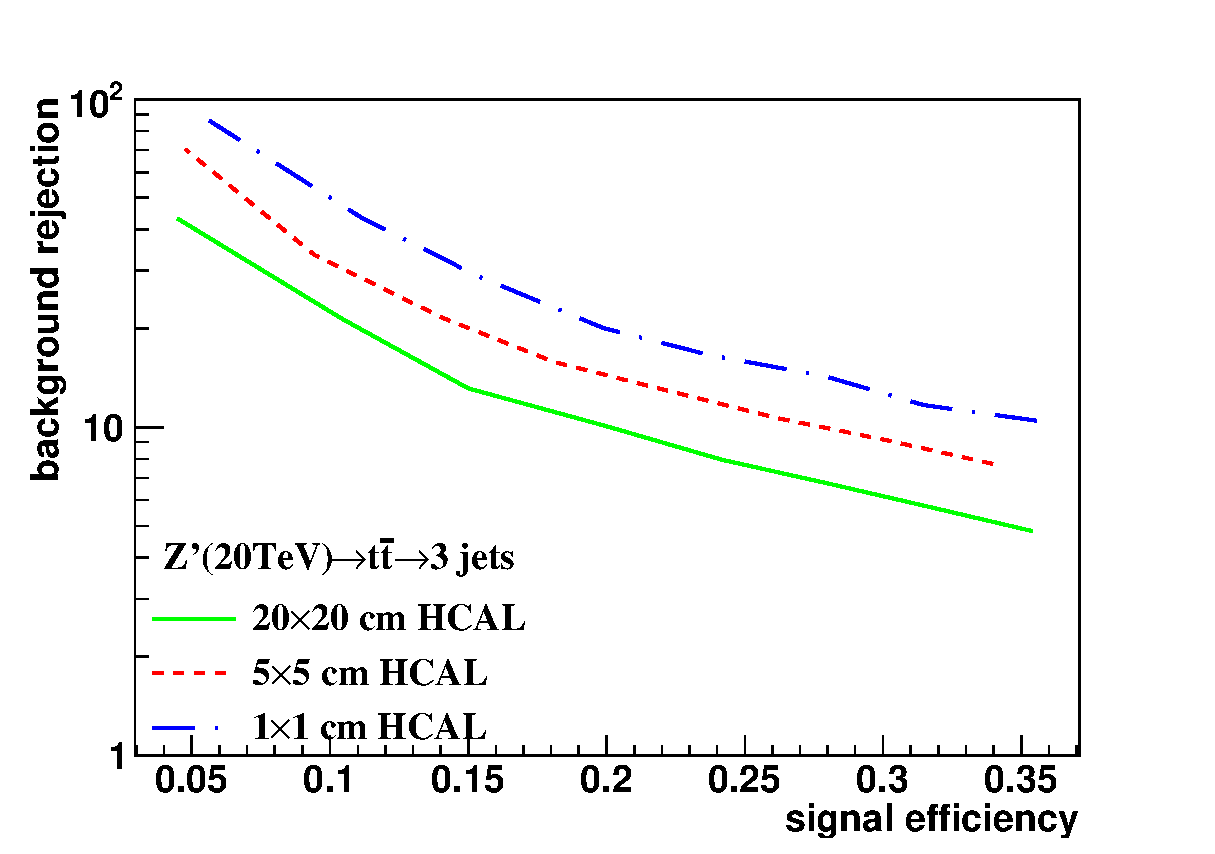
\includegraphics[width=0.43\textwidth]{figs/A_Cluster_mass_mmdt_20tev_eff_1_central_fix_tt_qq_log.eps}
 }
 \subfigure[Central at Median($20\times20$=190,$5\times5$=200,$1\times1$=190) change width in cluster at 40TeV] {
 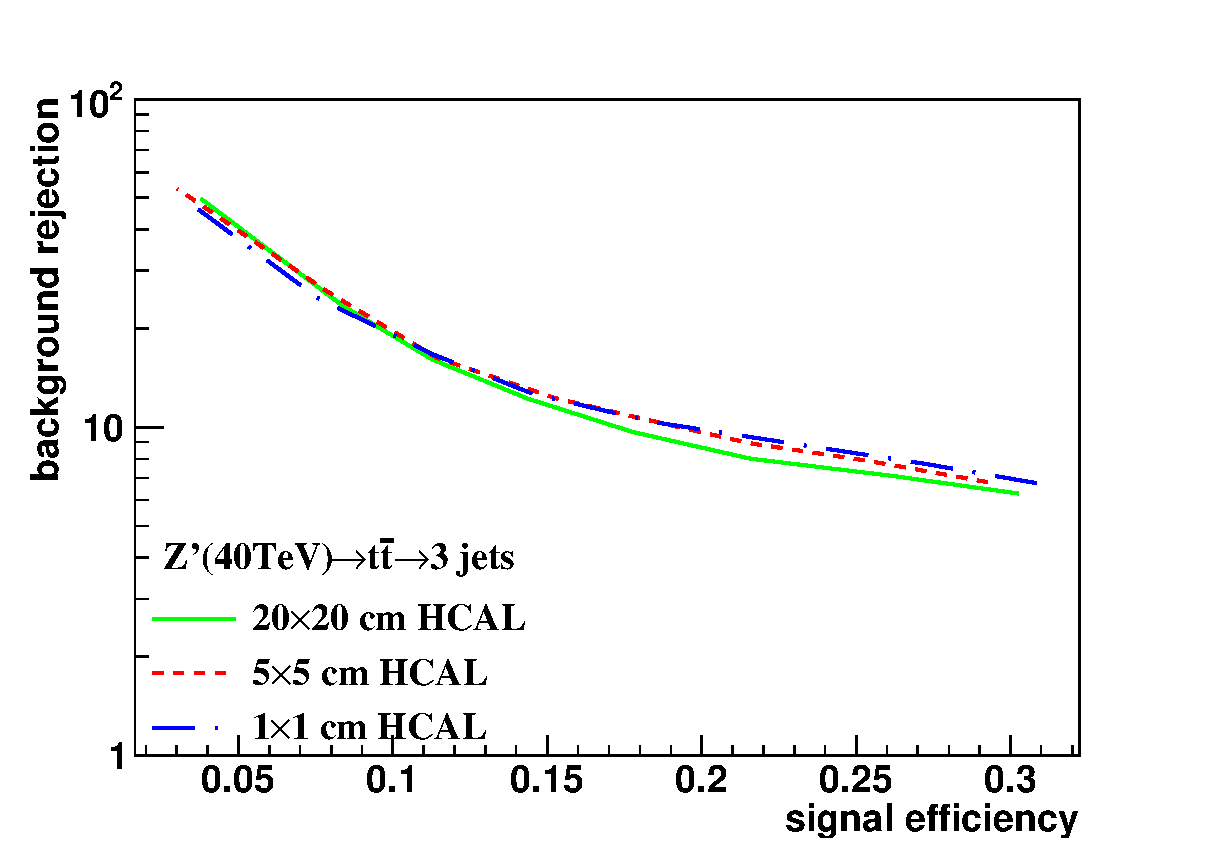
\includegraphics[width=0.43\textwidth]{figs/A_Cluster_mass_mmdt_40tev_eff_1_central_fix_tt_qq_log.eps}
 }
\end{center}
\caption{study of "fix central and change width" in mass soft drop at $\beta$=0, signal=tt, in 5, 10, 20, 40TeV energy of collision  in different detector sizes. Cell Size in 20$\times$20, 5$\times$5, and 1$\times$1(cm$\times$cm) are shown in each picture.}
\label{fig:cluster_tau21_tau32}
\end{figure}


\begin{figure}
\begin{center}
   \subfigure[5TeV at 20$\times$20(cm$\times$cm) in cluster] {
   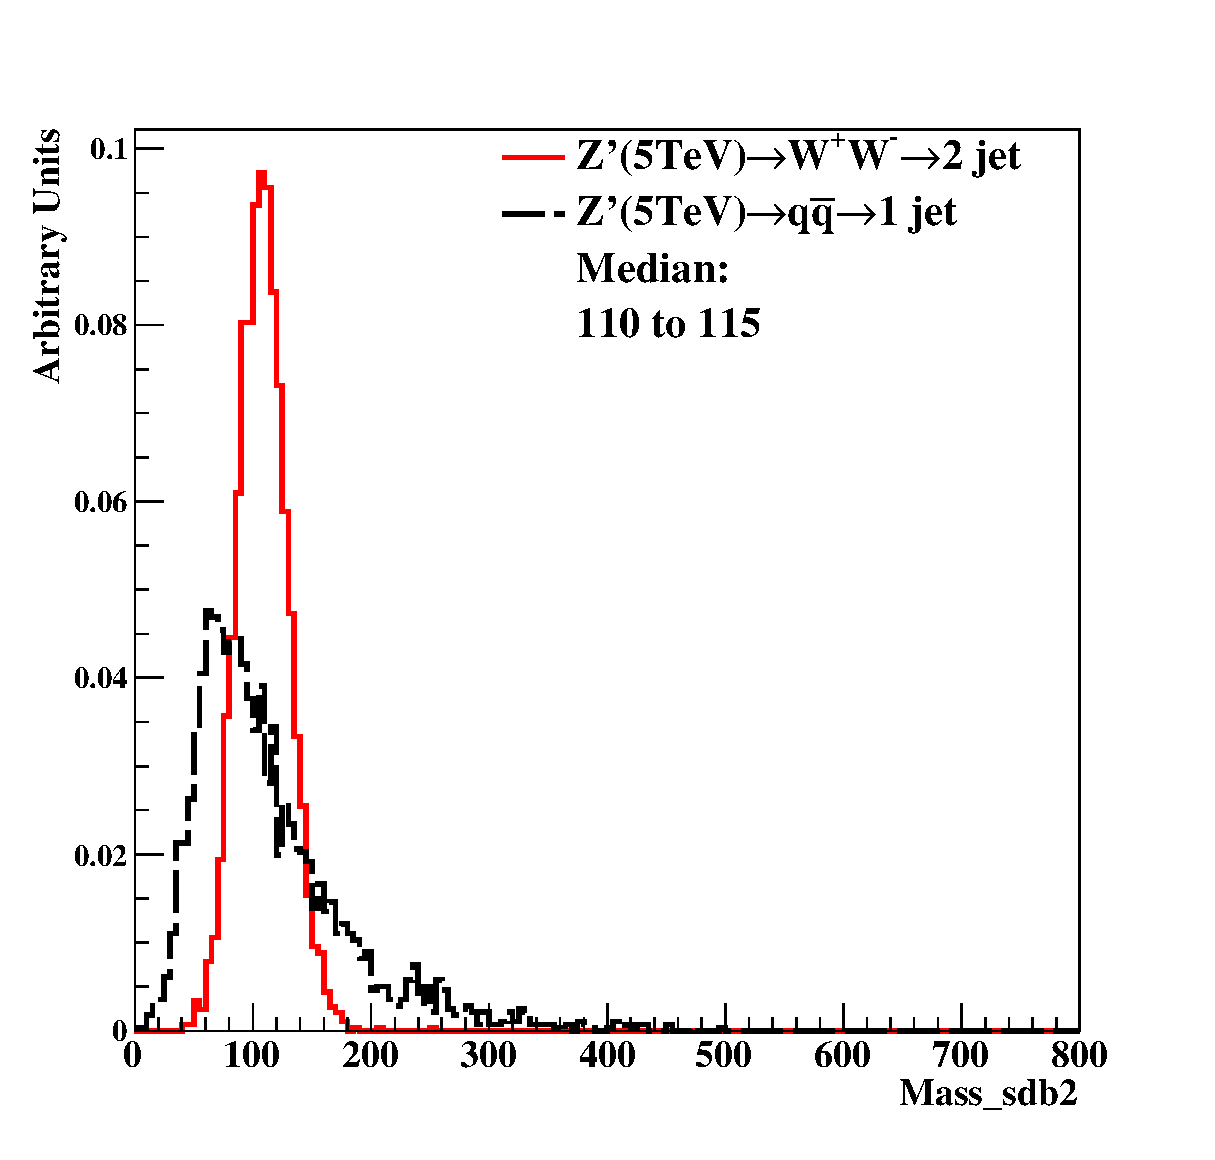
\includegraphics[width=0.22\textwidth]{figs/Dis_cluster_010_mass_sdb2_ww_5tev_04_800.eps}
   }
      \subfigure[10TeV at 20$\times$20(cm$\times$cm) in cluster] {
   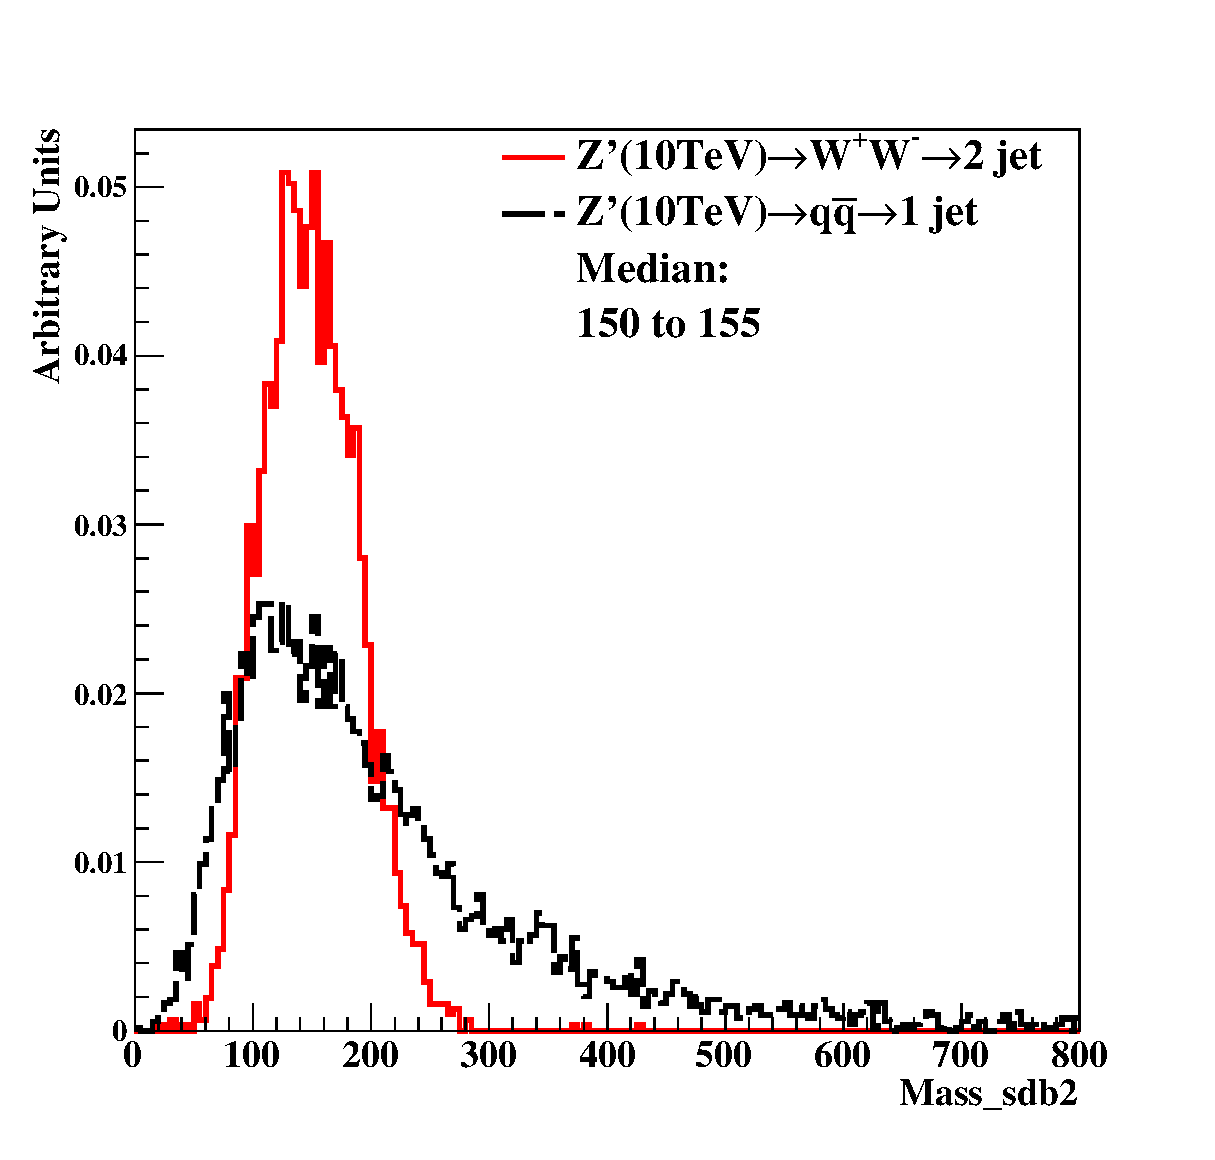
\includegraphics[width=0.22\textwidth]{figs/Dis_cluster_010_mass_sdb2_ww_10tev_04_800.eps}
   }
   \subfigure[20TeV at 20$\times$20(cm$\times$cm) in cluster] {
   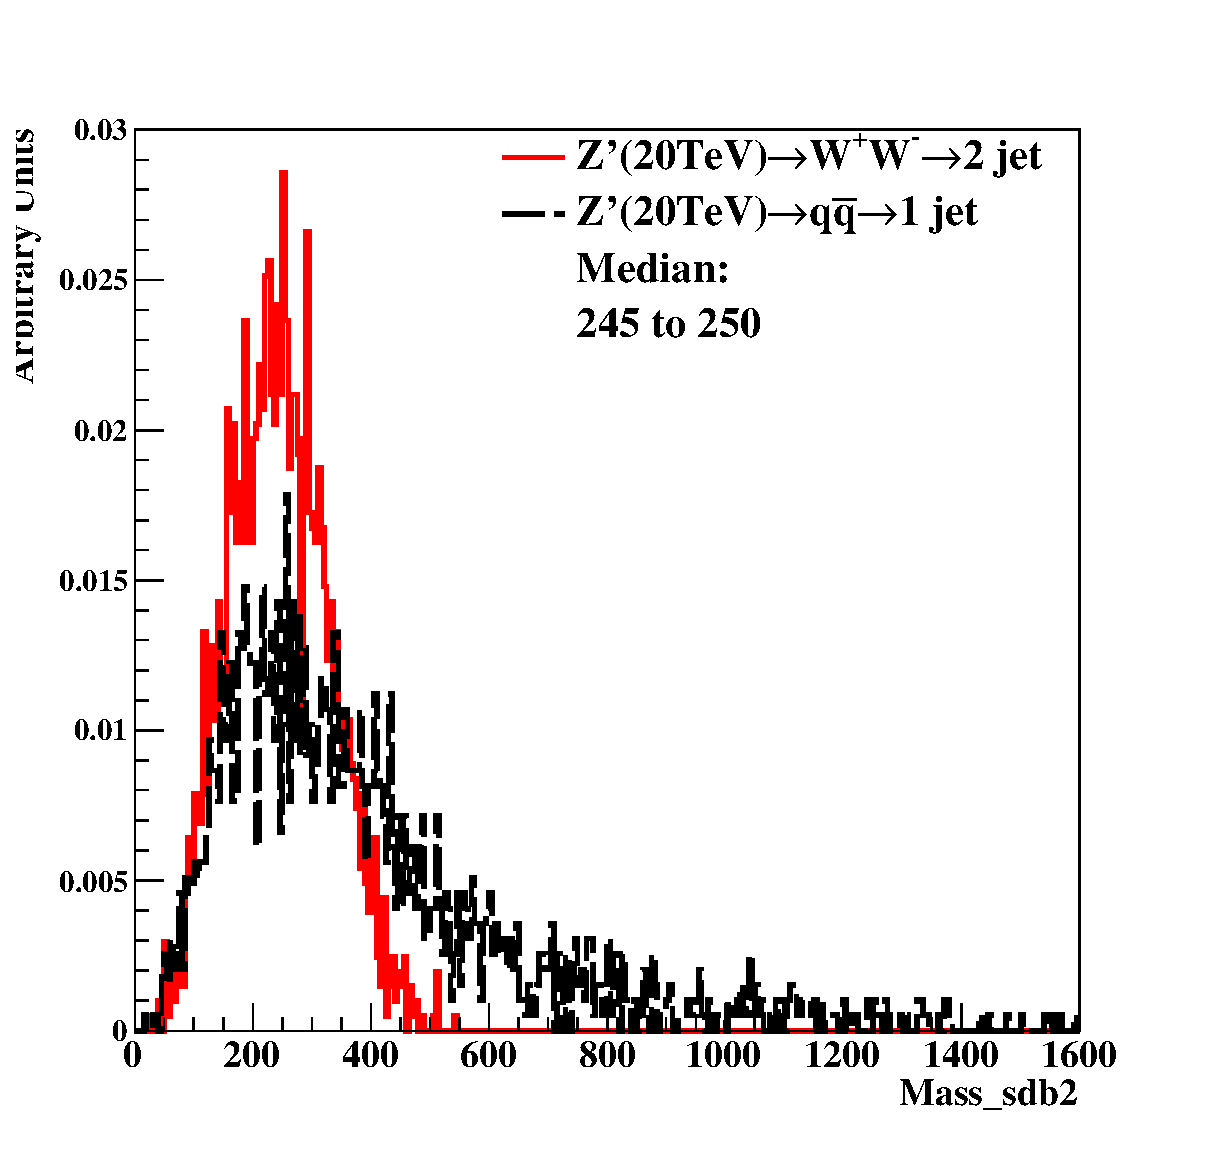
\includegraphics[width=0.22\textwidth]{figs/Dis_cluster_010_mass_sdb2_ww_20tev_04_1600.eps}
   }
    \subfigure[40TeV at 20$\times$20(cm$\times$cm) in cluster] {
   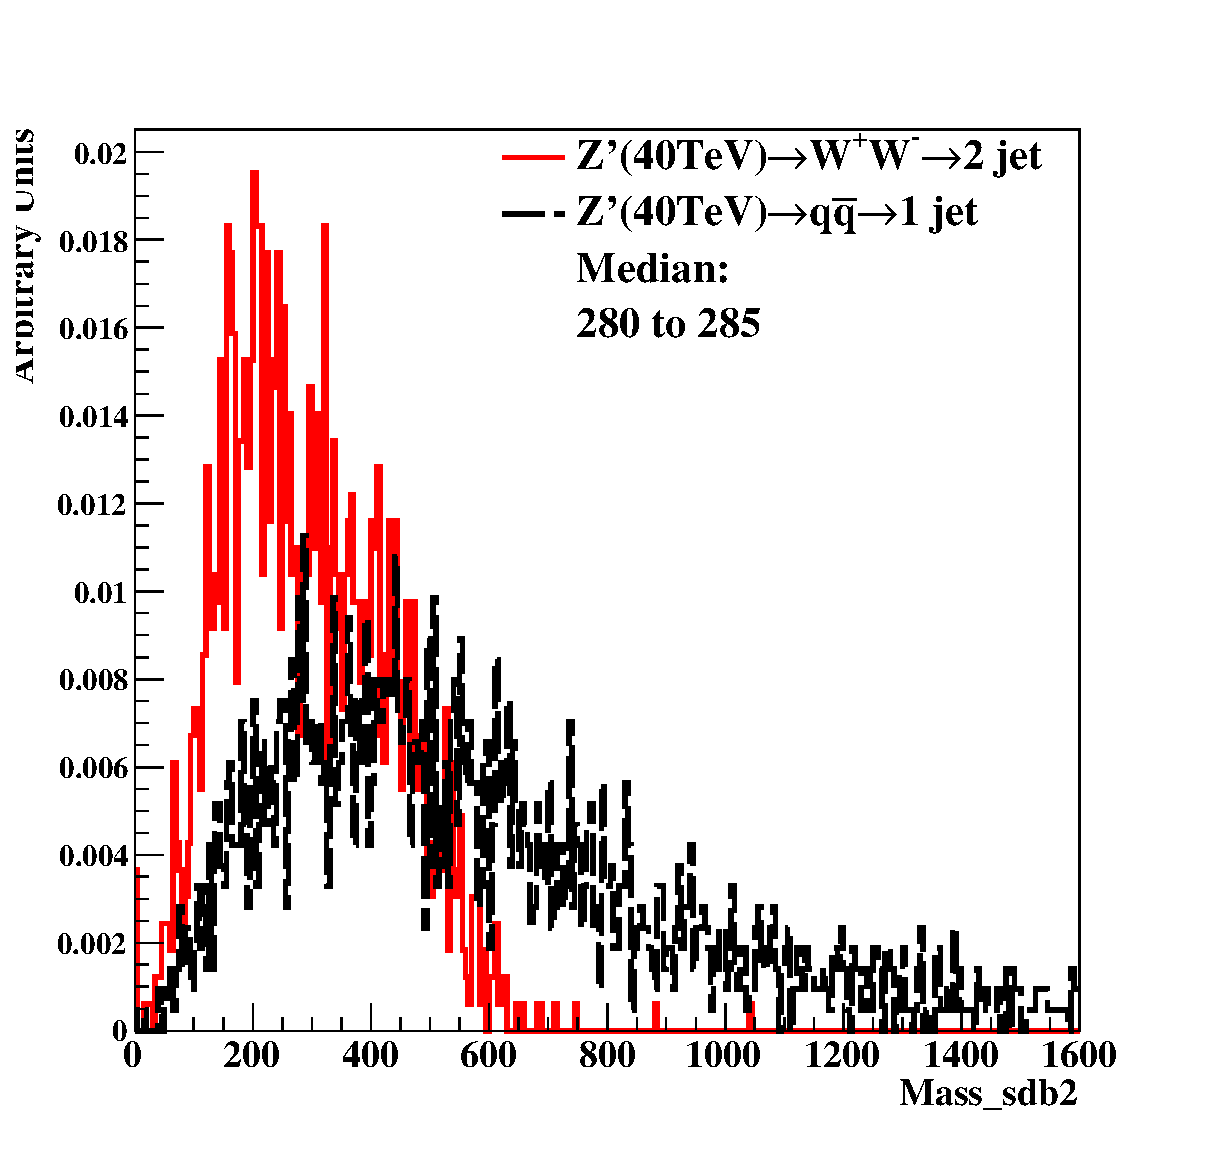
\includegraphics[width=0.22\textwidth]{figs/Dis_cluster_010_mass_sdb2_ww_40tev_04_1600.eps}
   }
   \subfigure[5TeV at 5$\times$5(cm$\times$cm) in cluster] {
   \includegraphics[width=0.22\textwidth]{figs/Dis_cluster_009_mass_sdb2_ww_5tev_04_800.eps}
   }
   \subfigure[10TeV at 5$\times$5(cm$\times$cm) in cluster] {
   \includegraphics[width=0.22\textwidth]{figs/Dis_cluster_009_mass_sdb2_ww_10tev_04_800.eps}
   }
    \subfigure[20TeV at 5$\times$5(cm$\times$cm) in cluster] {
   \includegraphics[width=0.22\textwidth]{figs/Dis_cluster_009_mass_sdb2_ww_20tev_04_1600.eps}\hfill
   }
      \subfigure[40TeV at 5$\times$5(cm$\times$cm) in cluster] {
   \includegraphics[width=0.22\textwidth]{figs/Dis_cluster_009_mass_sdb2_ww_40tev_04_1600.eps}\hfill
   }
   \subfigure[5TeV at 1$\times$1(cm$\times$cm) in cluster] {
   \includegraphics[width=0.22\textwidth]{figs/Dis_cluster_012_mass_sdb2_ww_5tev_04_800.eps}\hfill
   }
    \subfigure[10TeV at 1$\times$1(cm$\times$cm) in cluster] {
   \includegraphics[width=0.22\textwidth]{figs/Dis_cluster_012_mass_sdb2_ww_10tev_04_800.eps}
   }
   \subfigure[20TeV at 1$\times$1(cm$\times$cm) in cluster] {
   \includegraphics[width=0.22\textwidth]{figs/Dis_cluster_012_mass_sdb2_ww_20tev_04_1600.eps}\hfill
   }
      \subfigure[40TeV at 1$\times$1(cm$\times$cm) in cluster] {
   \includegraphics[width=0.22\textwidth]{figs/Dis_cluster_012_mass_sdb2_ww_40tev_04_1600.eps}
   }
\end{center}
\caption{Distributions of mass soft drop at $\beta$=2, signal=ww, in 5,10TeV energy of collision  in different detector sizes. Cell Size in 20$\times$20, 5$\times$5, and 1$\times$1(cm$\times$cm) are shown here.}
\label{fig:cluster_tau21_tau32}
\end{figure}


\begin{figure}
\begin{center}
  \subfigure[Central at Median($20\times20$=115,$5\times5$=110,$1\times1$=115) change width in cluster at 5TeV] {
  \includegraphics[width=0.43\textwidth]{figs/A_Cluster_mass_sdb2_5tev_eff_1_central_fix_ww_qq_log.eps}
  }
  \subfigure[Central at Median($20\times20$=155,$5\times5$=140,$1\times1$=145) change width in cluster at 10TeV] {
  \includegraphics[width=0.43\textwidth]{figs/A_Cluster_mass_sdb2_10tev_eff_1_central_fix_ww_qq_log.eps}
  }
 \subfigure[Central at Median($20\times20$=250,$5\times5$=195,$1\times1$=205) change width in cluster at 20TeV] {
 \includegraphics[width=0.43\textwidth]{figs/A_Cluster_mass_sdb2_20tev_eff_1_central_fix_ww_qq_log.eps}
 }
 \subfigure[Central at Median($20\times20$=285,$5\times5$=310,$1\times1$=290) change width in cluster at 40TeV] {
 \includegraphics[width=0.43\textwidth]{figs/A_Cluster_mass_sdb2_40tev_eff_1_central_fix_ww_qq_log.eps}
 }
\end{center}
\caption{study of "fix central and change width" in mass soft drop at $\beta$=2, signal=ww, in 5, 10, 20, 40TeV energy of collision  in different detector sizes. Cell Size in 20$\times$20, 5$\times$5, and 1$\times$1(cm$\times$cm) are shown in each picture.}
\label{fig:cluster_tau21_tau32}
\end{figure}

\begin{figure}
\begin{center}
   \subfigure[5TeV at 20$\times$20(cm$\times$cm) in cluster] {
   \includegraphics[width=0.22\textwidth]{figs/Dis_cluster_012_mass_sdb2_tt_5tev_04_tt_1200.eps}
   }
      \subfigure[10TeV at 20$\times$20(cm$\times$cm) in cluster] {
   \includegraphics[width=0.22\textwidth]{figs/Dis_cluster_010_mass_sdb2_tt_10tev_04_tt_1200.eps}
   }
   \subfigure[20TeV at 20$\times$20(cm$\times$cm) in cluster] {
   \includegraphics[width=0.22\textwidth]{figs/Dis_cluster_010_mass_sdb2_tt_20tev_04_tt_2400.eps}
   }
    \subfigure[40TeV at 20$\times$20(cm$\times$cm) in cluster] {
   \includegraphics[width=0.22\textwidth]{figs/Dis_cluster_010_mass_sdb2_tt_40tev_04_tt_2400.eps}
   }
   \subfigure[5TeV at 5$\times$5(cm$\times$cm) in cluster] {
   \includegraphics[width=0.22\textwidth]{figs/Dis_cluster_009_mass_sdb2_tt_5tev_04_tt_1200.eps}
   }
   \subfigure[10TeV at 5$\times$5(cm$\times$cm) in cluster] {
   \includegraphics[width=0.22\textwidth]{figs/Dis_cluster_009_mass_sdb2_tt_10tev_04_tt_1200.eps}
   }
   \subfigure[20TeV at 5$\times$5(cm$\times$cm) in cluster] {
   \includegraphics[width=0.22\textwidth]{figs/Dis_cluster_009_mass_sdb2_tt_20tev_04_tt_2400.eps}\hfill
   }
      \subfigure[40TeV at 5$\times$5(cm$\times$cm) in cluster] {
   \includegraphics[width=0.22\textwidth]{figs/Dis_cluster_009_mass_sdb2_tt_40tev_04_tt_2400.eps}\hfill
   }
   \subfigure[5TeV at 1$\times$1(cm$\times$cm) in cluster] {
   \includegraphics[width=0.22\textwidth]{figs/Dis_cluster_012_mass_sdb2_tt_5tev_04_tt_1200.eps}\hfill
   }
    \subfigure[10TeV at 1$\times$1(cm$\times$cm) in cluster] {
   \includegraphics[width=0.22\textwidth]{figs/Dis_cluster_012_mass_sdb2_tt_10tev_04_tt_1200.eps}
   }
   \subfigure[20TeV at 1$\times$1(cm$\times$cm) in cluster] {
   \includegraphics[width=0.22\textwidth]{figs/Dis_cluster_012_mass_sdb2_tt_20tev_04_tt_2400.eps}\hfill
   }
      \subfigure[40TeV at 1$\times$1(cm$\times$cm) in cluster] {
   \includegraphics[width=0.22\textwidth]{figs/Dis_cluster_012_mass_sdb2_tt_40tev_04_tt_2400.eps}
   }
\end{center}
\caption{Distributions of mass soft drop at $\beta$=2, signal=tt, in 5,10TeV energy of collision  in different detector sizes. Cell Size in 20$\times$20, 5$\times$5, and 1$\times$1(cm$\times$cm) are shown here.}
\label{fig:cluster_tau21_tau32}
\end{figure}


\begin{figure}
\begin{center}
  \subfigure[Central at Median($20\times20$=185,$5\times5$=185,$1\times1$=185) change width in cluster at 5TeV] {
  \includegraphics[width=0.43\textwidth]{figs/A_Cluster_mass_sdb2_5tev_eff_1_central_fix_tt_qq_log.eps}
  }
  \subfigure[Central at Median($20\times20$=240,$5\times5$=240,$1\times1$=240) change width in cluster at 10TeV] {
  \includegraphics[width=0.43\textwidth]{figs/A_Cluster_mass_sdb2_10tev_eff_1_central_fix_tt_qq_log.eps}
  }
 \subfigure[Central at Median($20\times20$=360,$5\times5$=375,$1\times1$=365) change width in cluster at 20TeV] {
 \includegraphics[width=0.43\textwidth]{figs/A_Cluster_mass_sdb2_20tev_eff_1_central_fix_tt_qq_log.eps}
 }
 \subfigure[Central at Median($20\times20$=620,$5\times5$=625,$1\times1$=630) change width in cluster at 40TeV] {
 \includegraphics[width=0.43\textwidth]{figs/A_Cluster_mass_sdb2_40tev_eff_1_central_fix_tt_qq_log.eps}
 }
\end{center}
\caption{study of "fix central and change width" in mass soft drop at $\beta$=2, signal=tt, in 5, 10, 20, 40TeV energy of collision  in different detector sizes. Cell Size in 20$\times$20, 5$\times$5, and 1$\times$1(cm$\times$cm) are shown in each picture.}
\label{fig:cluster_tau21_tau32}
\end{figure}







%yright 2007, 2008, 2009 Elsevier Ltd
%% 
%% This file is part of the 'Elsarticle Bundle'.
%% ---------------------------------------------
%% 
%% It may be distributed under the conditions of the LaTeX Project Public
%% License, either version 1.2 of this license or (at your option) any
%% later version.  The latest version of this license is in
%%    http://www.latex-project.org/lppl.txt
%% and version 1.2 or later is part of all distributions of LaTeX
%% version 1999/12/01 or later.
%% 
%% The list of all files belonging to the 'Elsarticle Bundle' is
%% given in the file `manifest.txt'.
%% 

%% Template article for Elsevier's document class `elsarticle'
%% with numbered style bibliographic references
%% SP 2008/03/01

% \documentclass[preprint,11pt]{elsarticle}
\section{Studies of signal and background separation using Mann-Whitney U test and some new methods}
%In this section, we study different jet substructure variables and compare their ability to separate the signal and the background for different detector sizes using Mann-Whitney U test.\\

%In the Mann Whitney U test by definition, if U value is closed to 0.5, it means two distributions have similar compositions, and we can't distinguish them very well. On the other hand, if U value of two distributions are closed to 0, it means both distributions' compositions are much different from each other. For another point of view, if U value is closed to 0.5, separation power of certain variable is bad, instead, if U value is closed to 0, separation power is great.\\

%Figure 6 shows the representative samples of the distributions about the U value for $\tau_{21}$,$\tau_{32}$ in different detector sizes. In $\tau_{21}$, separation power is improved when detector size is smaller, but in $\tau_{32}$, the smallest detector sizes isn't the best one to separate signal and background.\\

%In Figure 7, it shows the summary plots about the clustering in Mann Whitney U test in three different variables. In $\tau_{21}$, 5TeV has better separation power when detector sizes are getting smaller, but when energy higher than that, there is no improvement in smaller detector. In $\tau_{32}$, the case is similar to  $\tau_{21}$. Even worse, at some collision energies, bigger detector sizes have better separation power than smaller detector sizes. In $c_2^{(1)}$, all separation power aren't improved by detector sizes.  In summary, $c_2^{(1)}$ is the best parameter, because all values are smaller than other parameters compare with the same energy collision, and its separation power don't have the significant improvement in higher energy collision.\\

%In Figure 8 , it shows the summary plots about the rawhit cut at 0.5GeV in Mann Whitney U test in three different variables. In $\tau_{21}$, 5TeV and 10TeV have better separation power in smaller separation power, but when energy higher than that, it won't improve.  In $\tau_{32}$, all separation power aren't improved by detector sizes. In $c_2^{(1)}$, we can see in 5,10,20TeV, separation power will be improved slightly, but at 40TeV, it won't improve. In summary, $c_2^{(1)}$ has the highest power separation at highest collision energy.\\

%25bins

%25bins
\begin{figure}
\begin{center}
   \subfigure[5TeV at 20$\times$20(cm$\times$cm) in 0.5GeV] {
   \includegraphics[width=0.22\textwidth]{figs/Dis_Rawhit_05GeV_010_c2b1_5tev_04_after_cut_Man.eps}\hfill
   }
   \subfigure[10TeV at 20$\times$20(cm$\times$cm) in 0.5GeV] {
   \includegraphics[width=0.22\textwidth]{figs/Dis_Rawhit_05GeV_010_c2b1_10tev_04_after_cut_Man.eps}
   }
   \subfigure[20TeV at 20$\times$20(cm$\times$cm) in 0.5GeV] {
   \includegraphics[width=0.22\textwidth]{figs/Dis_Rawhit_05GeV_010_c2b1_20tev_04_after_cut_Man.eps}
   }
   \subfigure[40TeV at 20$\times$20(cm$\times$cm) in 0.5GeV] {
   \includegraphics[width=0.22\textwidth]{figs/Dis_Rawhit_05GeV_010_c2b1_40tev_04_after_cut_Man.eps}
   }
   \subfigure[5TeV at 5$\times$5(cm$\times$cm) in 0.5GeV] {
   \includegraphics[width=0.22\textwidth]{figs/Dis_Rawhit_05GeV_009_c2b1_5tev_04_after_cut_Man.eps}
   }
   \subfigure[10TeV at 5$\times$5(cm$\times$cm) in 0.5GeV] {
   \includegraphics[width=0.22\textwidth]{figs/Dis_Rawhit_05GeV_009_c2b1_10tev_04_after_cut_Man.eps}
   }
   \subfigure[20TeV at 5$\times$5(cm$\times$cm) in 0.5GeV] {
   \includegraphics[width=0.22\textwidth]{figs/Dis_Rawhit_05GeV_009_c2b1_20tev_04_after_cut_Man.eps}
   }
   \subfigure[40TeV at 5$\times$5(cm$\times$cm) in 0.5GeV] {
   \includegraphics[width=0.22\textwidth]{figs/Dis_Rawhit_05GeV_009_c2b1_40tev_04_after_cut_Man.eps}
   }
   \subfigure[5TeV at 1$\times$1(cm$\times$cm) in 0.5GeV] {
   \includegraphics[width=0.22\textwidth]{figs/Dis_Rawhit_05GeV_012_c2b1_5tev_04_after_cut_Man.eps}
   }
   \subfigure[10TeV at 1$\times$1(cm$\times$cm) in 0.5GeV] {
   \includegraphics[width=0.22\textwidth]{figs/Dis_Rawhit_05GeV_012_c2b1_10tev_04_after_cut_Man.eps}
   }
   \subfigure[20TeV at 1$\times$1(cm$\times$cm) in 0.5GeV] {
   \includegraphics[width=0.22\textwidth]{figs/Dis_Rawhit_05GeV_012_c2b1_20tev_04_after_cut_Man.eps}
   }
   \subfigure[40TeV at 1$\times$1(cm$\times$cm) in 0.5GeV] {
   \includegraphics[width=0.22\textwidth]{figs/Dis_Rawhit_05GeV_012_c2b1_40tev_04_after_cut_Man.eps}
   }\end{center}
\caption{Distributions of Mann-Whitney value U in 5, 10, 20, 40TeV energy collision for c2b1 in different detector sizes. Cell Size in 20$\times$20, 5$\times$5, and 1$\times$1(cm$\times$cm) are shown here.}
\label{fig:cluster_c2b1_tau32}
\end{figure}

\begin{figure}
\begin{center}
   \subfigure[5 TeV using Rawhit 0.5GeV cut method with New2 after cut Method] {
   \includegraphics[width=0.43\textwidth]{figs/Rawhit_05GeV_c2b1_5tev_eff_1_New2_after_cut_25bins.eps}\hfill
   }
   \subfigure[10 TeV using Rawhit 0.5GeV cut method with New2 after cut Method] {
   \includegraphics[width=0.43\textwidth]{figs/Rawhit_05GeV_c2b1_10tev_eff_1_New2_after_cut_25bins.eps}
   }
   \subfigure[20 TeV using Rawhit 0.5GeV cut method with New2 after cut Method] {
   \includegraphics[width=0.43\textwidth]{figs/Rawhit_05GeV_c2b1_20tev_eff_1_New2_after_cut_25bins.eps}
   }
   \subfigure[40 TeV using Rawhit 0.5GeV cut method with New2 after cut Method] {
   \includegraphics[width=0.43\textwidth]{figs/Rawhit_05GeV_c2b1_40tev_eff_1_New2_after_cut_25bins.eps}
   }
\end{center}
\caption{Signal efficiency versus background rejection rate using c2b1.The energies of collision at (a)5, (b)10, (c)20, (d)40TeV are shown here. In each picture, the three ROC curves correspond to different detector sizes.}
\label{fig:cluster_c2b1}
\end{figure}



%25bins
\begin{figure}
\begin{center}
   \subfigure[5TeV at 20$\times$20(cm$\times$cm) in 0.5GeV] {
   \includegraphics[width=0.22\textwidth]{figs/Dis_Rawhit_05GeV_010_tau21_5tev_04_after_cut_Man.eps}\hfill
   }
   \subfigure[10TeV at 20$\times$20(cm$\times$cm) in 0.5GeV] {
   \includegraphics[width=0.22\textwidth]{figs/Dis_Rawhit_05GeV_010_tau21_10tev_04_after_cut_Man.eps}
   }
   \subfigure[20TeV at 20$\times$20(cm$\times$cm) in 0.5GeV] {
   \includegraphics[width=0.22\textwidth]{figs/Dis_Rawhit_05GeV_010_tau21_20tev_04_after_cut_Man.eps}
   }
   \subfigure[40TeV at 20$\times$20(cm$\times$cm) in 0.5GeV] {
   \includegraphics[width=0.22\textwidth]{figs/Dis_Rawhit_05GeV_010_tau21_40tev_04_after_cut_Man.eps}
   }
   \subfigure[5TeV at 5$\times$5(cm$\times$cm) in 0.5GeV] {
   \includegraphics[width=0.22\textwidth]{figs/Dis_Rawhit_05GeV_009_tau21_5tev_04_after_cut_Man.eps}
   }
   \subfigure[10TeV at 5$\times$5(cm$\times$cm) in 0.5GeV] {
   \includegraphics[width=0.22\textwidth]{figs/Dis_Rawhit_05GeV_009_tau21_10tev_04_after_cut_Man.eps}
   }
   \subfigure[20TeV at 5$\times$5(cm$\times$cm) in 0.5GeV] {
   \includegraphics[width=0.22\textwidth]{figs/Dis_Rawhit_05GeV_009_tau21_20tev_04_after_cut_Man.eps}
   }
   \subfigure[40TeV at 5$\times$5(cm$\times$cm) in 0.5GeV] {
   \includegraphics[width=0.22\textwidth]{figs/Dis_Rawhit_05GeV_009_tau21_40tev_04_after_cut_Man.eps}
   }
   \subfigure[5TeV at 1$\times$1(cm$\times$cm) in 0.5GeV] {
   \includegraphics[width=0.22\textwidth]{figs/Dis_Rawhit_05GeV_012_tau21_5tev_04_after_cut_Man.eps}
   }
   \subfigure[10TeV at 1$\times$1(cm$\times$cm) in 0.5GeV] {
   \includegraphics[width=0.22\textwidth]{figs/Dis_Rawhit_05GeV_012_tau21_10tev_04_after_cut_Man.eps}
   }
   \subfigure[20TeV at 1$\times$1(cm$\times$cm) in 0.5GeV] {
   \includegraphics[width=0.22\textwidth]{figs/Dis_Rawhit_05GeV_012_tau21_20tev_04_after_cut_Man.eps}
   }
   \subfigure[40TeV at 1$\times$1(cm$\times$cm) in 0.5GeV] {
   \includegraphics[width=0.22\textwidth]{figs/Dis_Rawhit_05GeV_012_tau21_40tev_04_after_cut_Man.eps}
   }\end{center}
\caption{Distributions of Mann-Whitney value U in 5, 10, 20, 40TeV energy collision for $\tau_{21}$  in different detector sizes. Cell Size in 20$\times$20, 5$\times$5, and 1$\times$1(cm$\times$cm) are shown here.}
\label{fig:cluster_tau21_tau32}
\end{figure}
\begin{figure}
\begin{center}
   \subfigure[5 TeV using Rawhit 0.5GeV cut method with New2 after cut Method] {
   \includegraphics[width=0.43\textwidth]{figs/Rawhit_05GeV_tau21_5tev_eff_1_New2_after_cut_25bins.eps}\hfill
   }
   \subfigure[10 TeV using Rawhit 0.5GeV cut method with New2 after cut Method] {
   \includegraphics[width=0.43\textwidth]{figs/Rawhit_05GeV_tau21_10tev_eff_1_New2_after_cut_25bins.eps}
   }
   \subfigure[20 TeV using Rawhit 0.5GeV cut method with New2 after cut Method] {
   \includegraphics[width=0.43\textwidth]{figs/Rawhit_05GeV_tau21_20tev_eff_1_New2_after_cut_25bins.eps}
   }
   \subfigure[40 TeV using Rawhit 0.5GeV cut method with New2 after cut Method] {
   \includegraphics[width=0.43\textwidth]{figs/Rawhit_05GeV_tau21_40tev_eff_1_New2_after_cut_25bins.eps}
   }
\end{center}
\caption{Signal efficiency versus background rejection rate using $\tau_{21}$.The energies of collision at (a)5, (b)10, (c)20, (d)40TeV are shown here. In each picture, the three ROC curves correspond to different detector sizes.}
\label{fig:cluster_tau21}
\end{figure}




%25bins
\begin{figure}
\begin{center}
   \subfigure[5TeV at 20$\times$20(cm$\times$cm) in 0.5GeV] {
   \includegraphics[width=0.22\textwidth]{figs/Dis_Rawhit_05GeV_010_tau32_5tev_04_after_cut_Man.eps}\hfill
   }
   \subfigure[10TeV at 20$\times$20(cm$\times$cm) in 0.5GeV] {
   \includegraphics[width=0.22\textwidth]{figs/Dis_Rawhit_05GeV_010_tau32_10tev_04_after_cut_Man.eps}
   }
   \subfigure[20TeV at 20$\times$20(cm$\times$cm) in 0.5GeV] {
   \includegraphics[width=0.22\textwidth]{figs/Dis_Rawhit_05GeV_010_tau32_20tev_04_after_cut_Man.eps}
   }
   \subfigure[40TeV at 20$\times$20(cm$\times$cm) in 0.5GeV] {
   \includegraphics[width=0.22\textwidth]{figs/Dis_Rawhit_05GeV_010_tau32_40tev_04_after_cut_Man.eps}
   }
   \subfigure[5TeV at 5$\times$5(cm$\times$cm) in 0.5GeV] {
   \includegraphics[width=0.22\textwidth]{figs/Dis_Rawhit_05GeV_009_tau32_5tev_04_after_cut_Man.eps}
   }
   \subfigure[10TeV at 5$\times$5(cm$\times$cm) in 0.5GeV] {
   \includegraphics[width=0.22\textwidth]{figs/Dis_Rawhit_05GeV_009_tau32_10tev_04_after_cut_Man.eps}
   }
   \subfigure[20TeV at 5$\times$5(cm$\times$cm) in 0.5GeV] {
   \includegraphics[width=0.22\textwidth]{figs/Dis_Rawhit_05GeV_009_tau32_20tev_04_after_cut_Man.eps}
   }
   \subfigure[40TeV at 5$\times$5(cm$\times$cm) in 0.5GeV] {
   \includegraphics[width=0.22\textwidth]{figs/Dis_Rawhit_05GeV_009_tau32_40tev_04_after_cut_Man.eps}
   }
   \subfigure[5TeV at 1$\times$1(cm$\times$cm) in 0.5GeV] {
   \includegraphics[width=0.22\textwidth]{figs/Dis_Rawhit_05GeV_012_tau32_5tev_04_after_cut_Man.eps}
   }
   \subfigure[10TeV at 1$\times$1(cm$\times$cm) in 0.5GeV] {
   \includegraphics[width=0.22\textwidth]{figs/Dis_Rawhit_05GeV_012_tau32_10tev_04_after_cut_Man.eps}
   }
   \subfigure[20TeV at 1$\times$1(cm$\times$cm) in 0.5GeV] {
   \includegraphics[width=0.22\textwidth]{figs/Dis_Rawhit_05GeV_012_tau32_20tev_04_after_cut_Man.eps}
   }
   \subfigure[40TeV at 1$\times$1(cm$\times$cm) in 0.5GeV] {
   \includegraphics[width=0.22\textwidth]{figs/Dis_Rawhit_05GeV_012_tau32_40tev_04_after_cut_Man.eps}
   }\end{center}
\caption{Distributions of Mann-Whitney value U in 5, 10, 20, 40TeV energy collision for $\tau_{32}$  in different detector sizes. Cell Size in 20$\times$20, 5$\times$5, and 1$\times$1(cm$\times$cm) are shown here.}
\label{fig:cluster_tau32_tau32}
\end{figure}

\begin{figure}
\begin{center}
   \subfigure[5 TeV using Rawhit 0.5GeV cut method with New2 after cut Method] {
   \includegraphics[width=0.43\textwidth]{figs/Rawhit_05GeV_tau32_5tev_eff_1_New2_after_cut_25bins.eps}\hfill
   }
   \subfigure[10 TeV using Rawhit 0.5GeV cut method with New2 after cut Method] {
   \includegraphics[width=0.43\textwidth]{figs/Rawhit_05GeV_tau32_10tev_eff_1_New2_after_cut_25bins.eps}
   }
   \subfigure[20 TeV using Rawhit 0.5GeV cut method with New2 after cut Method] {
   \includegraphics[width=0.43\textwidth]{figs/Rawhit_05GeV_tau32_20tev_eff_1_New2_after_cut_25bins.eps}
   }
   \subfigure[40 TeV using Rawhit 0.5GeV cut method with New2 after cut Method] {
   \includegraphics[width=0.43\textwidth]{figs/Rawhit_05GeV_tau32_40tev_eff_1_New2_after_cut_25bins.eps}
   }
\end{center}
\caption{Signal efficiency versus background rejection rate using $\tau_{32}$.The energies of collision at (a)5, (b)10, (c)20, (d)40TeV are shown here. In each picture, the three ROC curves correspond to different detector sizes.}
\label{fig:cluster_tau32}
\end{figure}

%25bins

%25bins
%\begin{figure}
%\begin{center}
 %  \subfigure[5 TeV rawhit cut 0.5GeV compare with cluster]{
 %  \includegraphics[width=0.43\textwidth]{figs/Rawhit_025GeV_cluster_tau32_5tev_04_after_cut_eff_log.eps}\hfill
  % }
  % \subfigure[10 TeV rawhit cut 0.5GeV compare with cluster] {
  % \includegraphics[width=0.43\textwidth]{figs/Rawhit_025GeV_cluster_tau32_10tev_04_after_cut_eff_log.eps}
  % }
   %\subfigure[20 TeV rawhit cut 0.5GeV compare with cluster] {
   %\includegraphics[width=0.43\textwidth]{figs/Rawhit_025GeV_cluster_tau32_20tev_04_after_cut_eff_log.eps}
  % }
   %\subfigure[40 TeV rawhit cut 0.5GeV compare with cluster] {
   %\includegraphics[width=0.43\textwidth]{figs/Rawhit_025GeV_cluster_tau32_40tev_04_after_cut_eff_log.eps}
  % }
%\end{center}
%\caption{Signal efficiency versus background rejection rate using $\tau_{32}$.The energies of collision at (a)5, (b)10, (c)20, (d)40TeV are shown here. In each picture, the six ROC curves correspond to different detector sizes in different cut.}
%\label{fig:rawhit_0.5GeV_0.25GeV_tau32}
%\end{figure}



%25bins
\begin{figure}
\begin{center}
   \subfigure[$\tau_{21}$ rawhit cut at 0.5GeV] {
   \includegraphics[width=0.43\textwidth]{figs/raw_05_tau21_summary_U_after_cut_25bins.eps}\hfill
   }
   \subfigure[$\tau_{32}$ rawhit cut at 0.5GeV] {
   \includegraphics[width=0.43\textwidth]{figs/raw_05_tau32_summary_U_after_cut_25bins.eps}
   }
   \subfigure[$c_2^{(1)}$ rawhit cut at 0.5GeV] {
   \includegraphics[width=0.43\textwidth]{figs/raw_05_c2b1_summary_U_after_cut_25bins.eps}
   }
\end{center}
\caption{The Mann-Whitney U values for $\tau_{21}$,$\tau_{32}$ and $c_2^{(1)}$ reconstructed from calorimeter hit at 05GeV cut at different collision energies correspond to different detector sizes in rawhit cut at 05GeV. The energies of collision at 5, 10, 20, 40, 20, 40TeV are shown in each figure.}
\label{fig:raw_U_summary}
\end{figure}











\section*{Acknowledgements}
This research was performed using resources provided by the Open Science Grid,
which is supported by the National Science Foundation and the U.S. Department of Energy's Office of Science. 
We gratefully acknowledge the computing resources provided on Blues, 
a high-performance computing cluster operated by the Laboratory Computing Resource Center at Argonne National Laboratory.
Argonne National Laboratory's work was supported by the U.S. Department of Energy, Office of Science under contract DE-AC02-06CH11357.
The Fermi National Accelerator Laboratory (Fermilab) is operated by Fermi Research Alliance, LLC under Contract No. DE-AC02-07CH11359 with the United States Department of Energy.

\newpage
%%%%%%%%%%%%%%%%%%%%%% references %%%%%%%%%%%%%%%%%%%%%%%%%%%%%%
\section*{References}

\bibliographystyle{elsarticle-num}
\def\bibname{\Large\bf References}
\def\refname{\Large\bf References}
\pagestyle{plain}
\bibliography{biblio}



\end{document}
